\documentclass[twoside]{book}

% Packages required by doxygen
\usepackage{fixltx2e}
\usepackage{calc}
\usepackage{doxygen}
\usepackage[export]{adjustbox} % also loads graphicx
\usepackage{graphicx}
\usepackage[utf8]{inputenc}
\usepackage{makeidx}
\usepackage{multicol}
\usepackage{multirow}
\PassOptionsToPackage{warn}{textcomp}
\usepackage{textcomp}
\usepackage[nointegrals]{wasysym}
\usepackage[table]{xcolor}

% Font selection
\usepackage[T1]{fontenc}
\usepackage[scaled=.90]{helvet}
\usepackage{courier}
\usepackage{amssymb}
\usepackage{sectsty}
\renewcommand{\familydefault}{\sfdefault}
\allsectionsfont{%
  \fontseries{bc}\selectfont%
  \color{darkgray}%
}
\renewcommand{\DoxyLabelFont}{%
  \fontseries{bc}\selectfont%
  \color{darkgray}%
}
\newcommand{\+}{\discretionary{\mbox{\scriptsize$\hookleftarrow$}}{}{}}

% Page & text layout
\usepackage{geometry}
\geometry{%
  a4paper,%
  top=2.5cm,%
  bottom=2.5cm,%
  left=2.5cm,%
  right=2.5cm%
}
\tolerance=750
\hfuzz=15pt
\hbadness=750
\setlength{\emergencystretch}{15pt}
\setlength{\parindent}{0cm}
\setlength{\parskip}{3ex plus 2ex minus 2ex}
\makeatletter
\renewcommand{\paragraph}{%
  \@startsection{paragraph}{4}{0ex}{-1.0ex}{1.0ex}{%
    \normalfont\normalsize\bfseries\SS@parafont%
  }%
}
\renewcommand{\subparagraph}{%
  \@startsection{subparagraph}{5}{0ex}{-1.0ex}{1.0ex}{%
    \normalfont\normalsize\bfseries\SS@subparafont%
  }%
}
\makeatother

% Headers & footers
\usepackage{fancyhdr}
\pagestyle{fancyplain}
\fancyhead[LE]{\fancyplain{}{\bfseries\thepage}}
\fancyhead[CE]{\fancyplain{}{}}
\fancyhead[RE]{\fancyplain{}{\bfseries\leftmark}}
\fancyhead[LO]{\fancyplain{}{\bfseries\rightmark}}
\fancyhead[CO]{\fancyplain{}{}}
\fancyhead[RO]{\fancyplain{}{\bfseries\thepage}}
\fancyfoot[LE]{\fancyplain{}{}}
\fancyfoot[CE]{\fancyplain{}{}}
\fancyfoot[RE]{\fancyplain{}{\bfseries\scriptsize Generated by Doxygen }}
\fancyfoot[LO]{\fancyplain{}{\bfseries\scriptsize Generated by Doxygen }}
\fancyfoot[CO]{\fancyplain{}{}}
\fancyfoot[RO]{\fancyplain{}{}}
\renewcommand{\footrulewidth}{0.4pt}
\renewcommand{\chaptermark}[1]{%
  \markboth{#1}{}%
}
\renewcommand{\sectionmark}[1]{%
  \markright{\thesection\ #1}%
}

% Indices & bibliography
\usepackage{natbib}
\usepackage[titles]{tocloft}
\setcounter{tocdepth}{3}
\setcounter{secnumdepth}{5}
\makeindex

% Hyperlinks (required, but should be loaded last)
\usepackage{ifpdf}
\ifpdf
  \usepackage[pdftex,pagebackref=true]{hyperref}
\else
  \usepackage[ps2pdf,pagebackref=true]{hyperref}
\fi
\hypersetup{%
  colorlinks=true,%
  linkcolor=blue,%
  citecolor=blue,%
  unicode%
}

% Custom commands
\newcommand{\clearemptydoublepage}{%
  \newpage{\pagestyle{empty}\cleardoublepage}%
}

\usepackage{caption}
\captionsetup{labelsep=space,justification=centering,font={bf},singlelinecheck=off,skip=4pt,position=top}

%===== C O N T E N T S =====

\begin{document}

% Titlepage & ToC
\hypersetup{pageanchor=false,
             bookmarksnumbered=true,
             pdfencoding=unicode
            }
\pagenumbering{alph}
\begin{titlepage}
\vspace*{7cm}
\begin{center}%
{\Large Galactica Imanage App }\\
\vspace*{1cm}
{\large Generated by Doxygen 1.8.13}\\
\end{center}
\end{titlepage}
\clearemptydoublepage
\pagenumbering{roman}
\tableofcontents
\clearemptydoublepage
\pagenumbering{arabic}
\hypersetup{pageanchor=true}

%--- Begin generated contents ---
\chapter{Namespace Index}
\section{Namespace List}
Here is a list of all namespaces with brief descriptions\+:\begin{DoxyCompactList}
\item\contentsline{section}{\hyperlink{namespaceadmin}{admin} \\*Register models at admin }{\pageref{namespaceadmin}}{}
\item\contentsline{section}{\hyperlink{namespaceapps}{apps} \\*Imgapp app class }{\pageref{namespaceapps}}{}
\item\contentsline{section}{\hyperlink{namespaceExtractExif}{Extract\+Exif} \\*Extract meta-\/data from images }{\pageref{namespaceExtractExif}}{}
\item\contentsline{section}{\hyperlink{namespacefilebrowser__upload}{filebrowser\+\_\+upload} \\*Override the filebrowser site functionalities }{\pageref{namespacefilebrowser__upload}}{}
\item\contentsline{section}{\hyperlink{namespaceforms}{forms} \\*Model forms }{\pageref{namespaceforms}}{}
\item\contentsline{section}{\hyperlink{namespaceimgapp}{imgapp} }{\pageref{namespaceimgapp}}{}
\item\contentsline{section}{\hyperlink{namespaceimgapp_1_1admin}{imgapp.\+admin} }{\pageref{namespaceimgapp_1_1admin}}{}
\item\contentsline{section}{\hyperlink{namespaceimgapp_1_1apps}{imgapp.\+apps} }{\pageref{namespaceimgapp_1_1apps}}{}
\item\contentsline{section}{\hyperlink{namespaceimgapp_1_1ExtractExif}{imgapp.\+Extract\+Exif} }{\pageref{namespaceimgapp_1_1ExtractExif}}{}
\item\contentsline{section}{\hyperlink{namespaceimgapp_1_1filebrowser__upload}{imgapp.\+filebrowser\+\_\+upload} }{\pageref{namespaceimgapp_1_1filebrowser__upload}}{}
\item\contentsline{section}{\hyperlink{namespaceimgapp_1_1forms}{imgapp.\+forms} }{\pageref{namespaceimgapp_1_1forms}}{}
\item\contentsline{section}{\hyperlink{namespaceimgapp_1_1migrations}{imgapp.\+migrations} }{\pageref{namespaceimgapp_1_1migrations}}{}
\item\contentsline{section}{\hyperlink{namespaceimgapp_1_1migrations_1_10001__initial}{imgapp.\+migrations.\+0001\+\_\+initial} }{\pageref{namespaceimgapp_1_1migrations_1_10001__initial}}{}
\item\contentsline{section}{\hyperlink{namespaceimgapp_1_1migrations_1_10002__objects}{imgapp.\+migrations.\+0002\+\_\+objects} }{\pageref{namespaceimgapp_1_1migrations_1_10002__objects}}{}
\item\contentsline{section}{\hyperlink{namespaceimgapp_1_1migrations_1_10003__description}{imgapp.\+migrations.\+0003\+\_\+description} }{\pageref{namespaceimgapp_1_1migrations_1_10003__description}}{}
\item\contentsline{section}{\hyperlink{namespaceimgapp_1_1migrations_1_10004__auto__20190715__1327}{imgapp.\+migrations.\+0004\+\_\+auto\+\_\+20190715\+\_\+1327} }{\pageref{namespaceimgapp_1_1migrations_1_10004__auto__20190715__1327}}{}
\item\contentsline{section}{\hyperlink{namespaceimgapp_1_1models}{imgapp.\+models} }{\pageref{namespaceimgapp_1_1models}}{}
\item\contentsline{section}{\hyperlink{namespaceimgapp_1_1MongoQuery}{imgapp.\+Mongo\+Query} }{\pageref{namespaceimgapp_1_1MongoQuery}}{}
\item\contentsline{section}{\hyperlink{namespaceimgapp_1_1tests}{imgapp.\+tests} }{\pageref{namespaceimgapp_1_1tests}}{}
\item\contentsline{section}{\hyperlink{namespaceimgapp_1_1UpdateMongoDB}{imgapp.\+Update\+Mongo\+DB} }{\pageref{namespaceimgapp_1_1UpdateMongoDB}}{}
\item\contentsline{section}{\hyperlink{namespaceimgapp_1_1uploadCOCO}{imgapp.\+upload\+C\+O\+CO} }{\pageref{namespaceimgapp_1_1uploadCOCO}}{}
\item\contentsline{section}{\hyperlink{namespaceimgapp_1_1uploadThreadClass}{imgapp.\+upload\+Thread\+Class} }{\pageref{namespaceimgapp_1_1uploadThreadClass}}{}
\item\contentsline{section}{\hyperlink{namespaceimgapp_1_1urls}{imgapp.\+urls} }{\pageref{namespaceimgapp_1_1urls}}{}
\item\contentsline{section}{\hyperlink{namespaceimgapp_1_1utils}{imgapp.\+utils} }{\pageref{namespaceimgapp_1_1utils}}{}
\item\contentsline{section}{\hyperlink{namespaceimgapp_1_1views}{imgapp.\+views} }{\pageref{namespaceimgapp_1_1views}}{}
\item\contentsline{section}{\hyperlink{namespacemodels}{models} \\*Create your models here }{\pageref{namespacemodels}}{}
\item\contentsline{section}{\hyperlink{namespacemongoQuery}{mongo\+Query} \\*Module to query on mongo\+DB }{\pageref{namespacemongoQuery}}{}
\item\contentsline{section}{\hyperlink{namespaceUpdateMongoDB}{Update\+Mongo\+DB} \\*Utilities to update documents in Mongo\+DB }{\pageref{namespaceUpdateMongoDB}}{}
\item\contentsline{section}{\hyperlink{namespaceuploadThreadClass}{upload\+Thread\+Class} \\*Upload the metra data in a separate thread, (not being used in this imanage branch) }{\pageref{namespaceuploadThreadClass}}{}
\item\contentsline{section}{\hyperlink{namespaceutils}{utils} \\*All C\+O\+CO and darknet model functionalities }{\pageref{namespaceutils}}{}
\item\contentsline{section}{\hyperlink{namespaceviews}{views} \\*Handle requested views }{\pageref{namespaceviews}}{}
\end{DoxyCompactList}

\chapter{Hierarchical Index}
\section{Class Hierarchy}
This inheritance list is sorted roughly, but not completely, alphabetically\+:\begin{DoxyCompactList}
\item \contentsline{section}{imgapp.\+Extract\+Exif.\+extract\+Exif}{\pageref{classimgapp_1_1ExtractExif_1_1extractExif}}{}
\item \contentsline{section}{imgapp.\+forms.\+User\+Form.\+Meta}{\pageref{classimgapp_1_1forms_1_1UserForm_1_1Meta}}{}
\item \contentsline{section}{imgapp.\+forms.\+Profile\+Form.\+Meta}{\pageref{classimgapp_1_1forms_1_1ProfileForm_1_1Meta}}{}
\item Migration\begin{DoxyCompactList}
\item \contentsline{section}{imgapp.\+migrations.0001\+\_\+initial.Migration}{\pageref{classimgapp_1_1migrations_1_10001__initial_1_1Migration}}{}
\item \contentsline{section}{imgapp.\+migrations.0002\+\_\+objects.Migration}{\pageref{classimgapp_1_1migrations_1_10002__objects_1_1Migration}}{}
\item \contentsline{section}{imgapp.\+migrations.0003\+\_\+description.Migration}{\pageref{classimgapp_1_1migrations_1_10003__description_1_1Migration}}{}
\item \contentsline{section}{imgapp.\+migrations.0004\+\_\+auto\+\_\+20190715\+\_\+1327.Migration}{\pageref{classimgapp_1_1migrations_1_10004__auto__20190715__1327_1_1Migration}}{}
\end{DoxyCompactList}
\item Model\begin{DoxyCompactList}
\item \contentsline{section}{imgapp.\+models.\+Profile}{\pageref{classimgapp_1_1models_1_1Profile}}{}
\end{DoxyCompactList}
\item \contentsline{section}{imgapp.\+Mongo\+Query.\+mongo\+Query}{\pageref{classimgapp_1_1MongoQuery_1_1mongoQuery}}{}
\item Thread\begin{DoxyCompactList}
\item \contentsline{section}{imgapp.\+upload\+Thread\+Class.\+update\+Mongo\+Thread}{\pageref{classimgapp_1_1uploadThreadClass_1_1updateMongoThread}}{}
\end{DoxyCompactList}
\item \contentsline{section}{imgapp.\+utils.\+Utils}{\pageref{classimgapp_1_1utils_1_1Utils}}{}
\item App\+Config\begin{DoxyCompactList}
\item \contentsline{section}{imgapp.\+apps.\+Imgapp\+Config}{\pageref{classimgapp_1_1apps_1_1ImgappConfig}}{}
\end{DoxyCompactList}
\item File\+Browser\+Site\begin{DoxyCompactList}
\item \contentsline{section}{imgapp.\+filebrowser\+\_\+upload.\+user\+File\+Browser\+Site}{\pageref{classimgapp_1_1filebrowser__upload_1_1userFileBrowserSite}}{}
\end{DoxyCompactList}
\item Model\+Form\begin{DoxyCompactList}
\item \contentsline{section}{imgapp.\+forms.\+Profile\+Form}{\pageref{classimgapp_1_1forms_1_1ProfileForm}}{}
\item \contentsline{section}{imgapp.\+forms.\+User\+Form}{\pageref{classimgapp_1_1forms_1_1UserForm}}{}
\end{DoxyCompactList}
\end{DoxyCompactList}

\chapter{Class Index}
\section{Class List}
Here are the classes, structs, unions and interfaces with brief descriptions\+:\begin{DoxyCompactList}
\item\contentsline{section}{\hyperlink{classimgapp_1_1ExtractExif_1_1Extract__Exif}{imgapp.\+Extract\+Exif.\+Extract\+\_\+\+Exif} \\*\hyperlink{classimgapp_1_1ExtractExif_1_1Extract__Exif}{Extract\+\_\+\+Exif} class }{\pageref{classimgapp_1_1ExtractExif_1_1Extract__Exif}}{}
\item\contentsline{section}{\hyperlink{classimgapp_1_1apps_1_1ImgappConfig}{imgapp.\+apps.\+Imgapp\+Config} \\*Imgapp A\+PI class }{\pageref{classimgapp_1_1apps_1_1ImgappConfig}}{}
\item\contentsline{section}{\hyperlink{classimgapp_1_1forms_1_1UserForm_1_1Meta}{imgapp.\+forms.\+User\+Form.\+Meta} \\*\hyperlink{classimgapp_1_1forms_1_1UserForm_1_1Meta}{Meta} class }{\pageref{classimgapp_1_1forms_1_1UserForm_1_1Meta}}{}
\item\contentsline{section}{\hyperlink{classimgapp_1_1forms_1_1ProfileForm_1_1Meta}{imgapp.\+forms.\+Profile\+Form.\+Meta} \\*\hyperlink{classimgapp_1_1forms_1_1ProfileForm_1_1Meta}{Meta} class }{\pageref{classimgapp_1_1forms_1_1ProfileForm_1_1Meta}}{}
\item\contentsline{section}{\hyperlink{classimgapp_1_1migrations_1_10001__initial_1_1Migration}{imgapp.\+migrations.\+0001\+\_\+initial.\+Migration} }{\pageref{classimgapp_1_1migrations_1_10001__initial_1_1Migration}}{}
\item\contentsline{section}{\hyperlink{classimgapp_1_1migrations_1_10002__objects_1_1Migration}{imgapp.\+migrations.\+0002\+\_\+objects.\+Migration} }{\pageref{classimgapp_1_1migrations_1_10002__objects_1_1Migration}}{}
\item\contentsline{section}{\hyperlink{classimgapp_1_1migrations_1_10003__description_1_1Migration}{imgapp.\+migrations.\+0003\+\_\+description.\+Migration} }{\pageref{classimgapp_1_1migrations_1_10003__description_1_1Migration}}{}
\item\contentsline{section}{\hyperlink{classimgapp_1_1MongoQuery_1_1MongoQuery}{imgapp.\+Mongo\+Query.\+Mongo\+Query} \\*Class to query mongo\+DB }{\pageref{classimgapp_1_1MongoQuery_1_1MongoQuery}}{}
\item\contentsline{section}{\hyperlink{classimgapp_1_1models_1_1Profile}{imgapp.\+models.\+Profile} \\*User \hyperlink{classimgapp_1_1models_1_1Profile}{Profile} }{\pageref{classimgapp_1_1models_1_1Profile}}{}
\item\contentsline{section}{\hyperlink{classimgapp_1_1forms_1_1ProfileForm}{imgapp.\+forms.\+Profile\+Form} \\*\hyperlink{classimgapp_1_1forms_1_1ProfileForm}{Profile\+Form} }{\pageref{classimgapp_1_1forms_1_1ProfileForm}}{}
\item\contentsline{section}{\hyperlink{classimgapp_1_1uploadThreadClass_1_1UpdateMongo__Thread}{imgapp.\+upload\+Thread\+Class.\+Update\+Mongo\+\_\+\+Thread} \\*Class to update mongo\+DB }{\pageref{classimgapp_1_1uploadThreadClass_1_1UpdateMongo__Thread}}{}
\item\contentsline{section}{\hyperlink{classimgapp_1_1filebrowser__upload_1_1UserFileBrowserSite}{imgapp.\+filebrowser\+\_\+upload.\+User\+File\+Browser\+Site} \\*Override filebrowser site functionalities }{\pageref{classimgapp_1_1filebrowser__upload_1_1UserFileBrowserSite}}{}
\item\contentsline{section}{\hyperlink{classimgapp_1_1forms_1_1UserForm}{imgapp.\+forms.\+User\+Form} \\*\hyperlink{classimgapp_1_1forms_1_1UserForm}{User\+Form} }{\pageref{classimgapp_1_1forms_1_1UserForm}}{}
\item\contentsline{section}{\hyperlink{classimgapp_1_1utils_1_1Utils}{imgapp.\+utils.\+Utils} \\*Darknet model class }{\pageref{classimgapp_1_1utils_1_1Utils}}{}
\end{DoxyCompactList}

\chapter{File Index}
\section{File List}
Here is a list of all files with brief descriptions\+:\begin{DoxyCompactList}
\item\contentsline{section}{imgapp/\hyperlink{____init_____8py}{\+\_\+\+\_\+init\+\_\+\+\_\+.\+py} }{\pageref{____init_____8py}}{}
\item\contentsline{section}{imgapp/\hyperlink{admin_8py}{admin.\+py} }{\pageref{admin_8py}}{}
\item\contentsline{section}{imgapp/\hyperlink{apps_8py}{apps.\+py} }{\pageref{apps_8py}}{}
\item\contentsline{section}{imgapp/\hyperlink{ExtractExif_8py}{Extract\+Exif.\+py} }{\pageref{ExtractExif_8py}}{}
\item\contentsline{section}{imgapp/\hyperlink{filebrowser__upload_8py}{filebrowser\+\_\+upload.\+py} }{\pageref{filebrowser__upload_8py}}{}
\item\contentsline{section}{imgapp/\hyperlink{forms_8py}{forms.\+py} }{\pageref{forms_8py}}{}
\item\contentsline{section}{imgapp/\hyperlink{models_8py}{models.\+py} }{\pageref{models_8py}}{}
\item\contentsline{section}{imgapp/\hyperlink{MongoQuery_8py}{Mongo\+Query.\+py} }{\pageref{MongoQuery_8py}}{}
\item\contentsline{section}{imgapp/\hyperlink{tests_8py}{tests.\+py} }{\pageref{tests_8py}}{}
\item\contentsline{section}{imgapp/\hyperlink{UpdateMongoDB_8py}{Update\+Mongo\+D\+B.\+py} }{\pageref{UpdateMongoDB_8py}}{}
\item\contentsline{section}{imgapp/\hyperlink{uploadCOCO_8py}{upload\+C\+O\+C\+O.\+py} }{\pageref{uploadCOCO_8py}}{}
\item\contentsline{section}{imgapp/\hyperlink{uploadThreadClass_8py}{upload\+Thread\+Class.\+py} }{\pageref{uploadThreadClass_8py}}{}
\item\contentsline{section}{imgapp/\hyperlink{urls_8py}{urls.\+py} }{\pageref{urls_8py}}{}
\item\contentsline{section}{imgapp/\hyperlink{utils_8py}{utils.\+py} }{\pageref{utils_8py}}{}
\item\contentsline{section}{imgapp/\hyperlink{views_8py}{views.\+py} }{\pageref{views_8py}}{}
\item\contentsline{section}{imgapp/migrations/\hyperlink{0001__initial_8py}{0001\+\_\+initial.\+py} }{\pageref{0001__initial_8py}}{}
\item\contentsline{section}{imgapp/migrations/\hyperlink{0002__objects_8py}{0002\+\_\+objects.\+py} }{\pageref{0002__objects_8py}}{}
\item\contentsline{section}{imgapp/migrations/\hyperlink{0003__description_8py}{0003\+\_\+description.\+py} }{\pageref{0003__description_8py}}{}
\item\contentsline{section}{imgapp/migrations/\hyperlink{0004__auto__20190715__1327_8py}{0004\+\_\+auto\+\_\+20190715\+\_\+1327.\+py} }{\pageref{0004__auto__20190715__1327_8py}}{}
\item\contentsline{section}{imgapp/migrations/\hyperlink{migrations_2____init_____8py}{\+\_\+\+\_\+init\+\_\+\+\_\+.\+py} }{\pageref{migrations_2____init_____8py}}{}
\end{DoxyCompactList}

\chapter{Namespace Documentation}
\hypertarget{namespaceadmin}{}\section{admin Namespace Reference}
\label{namespaceadmin}\index{admin@{admin}}


register models at admin  




\subsection{Detailed Description}
register models at admin 
\hypertarget{namespaceapps}{}\section{apps Namespace Reference}
\label{namespaceapps}\index{apps@{apps}}


imgapp app class  




\subsection{Detailed Description}
imgapp app class 
\hypertarget{namespaceExtractExif}{}\section{Extract\+Exif Namespace Reference}
\label{namespaceExtractExif}\index{Extract\+Exif@{Extract\+Exif}}


extract meta-\/data from images.  




\subsection{Detailed Description}
extract meta-\/data from images. 

returns meta-\/data in json format. 
\hypertarget{namespacefilebrowser__upload}{}\section{filebrowser\+\_\+upload Namespace Reference}
\label{namespacefilebrowser__upload}\index{filebrowser\+\_\+upload@{filebrowser\+\_\+upload}}


override the filebrowser site functionalities  




\subsection{Detailed Description}
override the filebrowser site functionalities 
\hypertarget{namespaceforms}{}\section{forms Namespace Reference}
\label{namespaceforms}\index{forms@{forms}}


model forms  




\subsection{Detailed Description}
model forms 
\hypertarget{namespaceimgapp}{}\section{imgapp Namespace Reference}
\label{namespaceimgapp}\index{imgapp@{imgapp}}
\subsection*{Namespaces}
\begin{DoxyCompactItemize}
\item 
 \hyperlink{namespaceimgapp_1_1admin}{admin}
\item 
 \hyperlink{namespaceimgapp_1_1apps}{apps}
\item 
 \hyperlink{namespaceimgapp_1_1ExtractExif}{Extract\+Exif}
\item 
 \hyperlink{namespaceimgapp_1_1filebrowser__upload}{filebrowser\+\_\+upload}
\item 
 \hyperlink{namespaceimgapp_1_1forms}{forms}
\item 
 \hyperlink{namespaceimgapp_1_1migrations}{migrations}
\item 
 \hyperlink{namespaceimgapp_1_1models}{models}
\item 
 \hyperlink{namespaceimgapp_1_1MongoQuery}{Mongo\+Query}
\item 
 \hyperlink{namespaceimgapp_1_1tests}{tests}
\item 
 \hyperlink{namespaceimgapp_1_1UpdateMongoDB}{Update\+Mongo\+DB}
\item 
 \hyperlink{namespaceimgapp_1_1uploadCOCO}{upload\+C\+O\+CO}
\item 
 \hyperlink{namespaceimgapp_1_1uploadThreadClass}{upload\+Thread\+Class}
\item 
 \hyperlink{namespaceimgapp_1_1urls}{urls}
\item 
 \hyperlink{namespaceimgapp_1_1utils}{utils}
\item 
 \hyperlink{namespaceimgapp_1_1views}{views}
\end{DoxyCompactItemize}

\hypertarget{namespaceimgapp_1_1admin}{}\section{imgapp.\+admin Namespace Reference}
\label{namespaceimgapp_1_1admin}\index{imgapp.\+admin@{imgapp.\+admin}}

\hypertarget{namespaceimgapp_1_1apps}{}\section{imgapp.\+apps Namespace Reference}
\label{namespaceimgapp_1_1apps}\index{imgapp.\+apps@{imgapp.\+apps}}
\subsection*{Classes}
\begin{DoxyCompactItemize}
\item 
class \hyperlink{classimgapp_1_1apps_1_1ImgappConfig}{Imgapp\+Config}
\begin{DoxyCompactList}\small\item\em imgapp A\+PI class \end{DoxyCompactList}\end{DoxyCompactItemize}

\hypertarget{namespaceimgapp_1_1ExtractExif}{}\section{imgapp.\+Extract\+Exif Namespace Reference}
\label{namespaceimgapp_1_1ExtractExif}\index{imgapp.\+Extract\+Exif@{imgapp.\+Extract\+Exif}}
\subsection*{Classes}
\begin{DoxyCompactItemize}
\item 
class \hyperlink{classimgapp_1_1ExtractExif_1_1extractExif}{extract\+Exif}
\begin{DoxyCompactList}\small\item\em \hyperlink{classimgapp_1_1ExtractExif_1_1extractExif}{extract\+Exif} class \end{DoxyCompactList}\end{DoxyCompactItemize}

\hypertarget{namespaceimgapp_1_1filebrowser__upload}{}\section{imgapp.\+filebrowser\+\_\+upload Namespace Reference}
\label{namespaceimgapp_1_1filebrowser__upload}\index{imgapp.\+filebrowser\+\_\+upload@{imgapp.\+filebrowser\+\_\+upload}}
\subsection*{Classes}
\begin{DoxyCompactItemize}
\item 
class \hyperlink{classimgapp_1_1filebrowser__upload_1_1UserFileBrowserSite}{User\+File\+Browser\+Site}
\begin{DoxyCompactList}\small\item\em Override filebrowser site functionalities. \end{DoxyCompactList}\end{DoxyCompactItemize}
\subsection*{Variables}
\begin{DoxyCompactItemize}
\item 
\hyperlink{namespaceimgapp_1_1filebrowser__upload_ae26049c70fbfba51dec84d62840e6a01}{storage} = Default\+Storage()
\item 
\hyperlink{namespaceimgapp_1_1filebrowser__upload_a4f8619d5576e067e06247f18cd273af8}{site} = \hyperlink{classimgapp_1_1filebrowser__upload_1_1UserFileBrowserSite}{User\+File\+Browser\+Site}(name=\textquotesingle{}filebrowser\textquotesingle{}, \hyperlink{namespaceimgapp_1_1filebrowser__upload_ae26049c70fbfba51dec84d62840e6a01}{storage}=\hyperlink{namespaceimgapp_1_1filebrowser__upload_ae26049c70fbfba51dec84d62840e6a01}{storage})
\end{DoxyCompactItemize}


\subsection{Variable Documentation}
\mbox{\Hypertarget{namespaceimgapp_1_1filebrowser__upload_a4f8619d5576e067e06247f18cd273af8}\label{namespaceimgapp_1_1filebrowser__upload_a4f8619d5576e067e06247f18cd273af8}} 
\index{imgapp\+::filebrowser\+\_\+upload@{imgapp\+::filebrowser\+\_\+upload}!site@{site}}
\index{site@{site}!imgapp\+::filebrowser\+\_\+upload@{imgapp\+::filebrowser\+\_\+upload}}
\subsubsection{\texorpdfstring{site}{site}}
{\footnotesize\ttfamily imgapp.\+filebrowser\+\_\+upload.\+site = \hyperlink{classimgapp_1_1filebrowser__upload_1_1UserFileBrowserSite}{User\+File\+Browser\+Site}(name=\textquotesingle{}filebrowser\textquotesingle{}, \hyperlink{namespaceimgapp_1_1filebrowser__upload_ae26049c70fbfba51dec84d62840e6a01}{storage}=\hyperlink{namespaceimgapp_1_1filebrowser__upload_ae26049c70fbfba51dec84d62840e6a01}{storage})}

\mbox{\Hypertarget{namespaceimgapp_1_1filebrowser__upload_ae26049c70fbfba51dec84d62840e6a01}\label{namespaceimgapp_1_1filebrowser__upload_ae26049c70fbfba51dec84d62840e6a01}} 
\index{imgapp\+::filebrowser\+\_\+upload@{imgapp\+::filebrowser\+\_\+upload}!storage@{storage}}
\index{storage@{storage}!imgapp\+::filebrowser\+\_\+upload@{imgapp\+::filebrowser\+\_\+upload}}
\subsubsection{\texorpdfstring{storage}{storage}}
{\footnotesize\ttfamily imgapp.\+filebrowser\+\_\+upload.\+storage = Default\+Storage()}


\hypertarget{namespaceimgapp_1_1forms}{}\section{imgapp.\+forms Namespace Reference}
\label{namespaceimgapp_1_1forms}\index{imgapp.\+forms@{imgapp.\+forms}}
\subsection*{Classes}
\begin{DoxyCompactItemize}
\item 
class \hyperlink{classimgapp_1_1forms_1_1ProfileForm}{Profile\+Form}
\begin{DoxyCompactList}\small\item\em \hyperlink{classimgapp_1_1forms_1_1ProfileForm}{Profile\+Form}. \end{DoxyCompactList}\item 
class \hyperlink{classimgapp_1_1forms_1_1UserForm}{User\+Form}
\begin{DoxyCompactList}\small\item\em \hyperlink{classimgapp_1_1forms_1_1UserForm}{User\+Form}. \end{DoxyCompactList}\end{DoxyCompactItemize}

\hypertarget{namespaceimgapp_1_1migrations}{}\section{imgapp.\+migrations Namespace Reference}
\label{namespaceimgapp_1_1migrations}\index{imgapp.\+migrations@{imgapp.\+migrations}}
\subsection*{Namespaces}
\begin{DoxyCompactItemize}
\item 
 \hyperlink{namespaceimgapp_1_1migrations_1_10001__initial}{0001\+\_\+initial}
\item 
 \hyperlink{namespaceimgapp_1_1migrations_1_10002__objects}{0002\+\_\+objects}
\item 
 \hyperlink{namespaceimgapp_1_1migrations_1_10003__description}{0003\+\_\+description}
\item 
 \hyperlink{namespaceimgapp_1_1migrations_1_10004__auto__20190715__1327}{0004\+\_\+auto\+\_\+20190715\+\_\+1327}
\end{DoxyCompactItemize}

\hypertarget{namespaceimgapp_1_1migrations_1_10001__initial}{}\section{imgapp.\+migrations.0001\+\_\+initial Namespace Reference}
\label{namespaceimgapp_1_1migrations_1_10001__initial}\index{imgapp.\+migrations.\+0001\+\_\+initial@{imgapp.\+migrations.\+0001\+\_\+initial}}
\subsection*{Classes}
\begin{DoxyCompactItemize}
\item 
class \hyperlink{classimgapp_1_1migrations_1_10001__initial_1_1Migration}{Migration}
\end{DoxyCompactItemize}

\hypertarget{namespaceimgapp_1_1migrations_1_10002__objects}{}\section{imgapp.\+migrations.0002\+\_\+objects Namespace Reference}
\label{namespaceimgapp_1_1migrations_1_10002__objects}\index{imgapp.\+migrations.\+0002\+\_\+objects@{imgapp.\+migrations.\+0002\+\_\+objects}}
\subsection*{Classes}
\begin{DoxyCompactItemize}
\item 
class \hyperlink{classimgapp_1_1migrations_1_10002__objects_1_1Migration}{Migration}
\end{DoxyCompactItemize}

\hypertarget{namespaceimgapp_1_1migrations_1_10003__description}{}\section{imgapp.\+migrations.0003\+\_\+description Namespace Reference}
\label{namespaceimgapp_1_1migrations_1_10003__description}\index{imgapp.\+migrations.\+0003\+\_\+description@{imgapp.\+migrations.\+0003\+\_\+description}}
\subsection*{Classes}
\begin{DoxyCompactItemize}
\item 
class \hyperlink{classimgapp_1_1migrations_1_10003__description_1_1Migration}{Migration}
\end{DoxyCompactItemize}

\hypertarget{namespaceimgapp_1_1migrations_1_10004__auto__20190715__1327}{}\section{imgapp.\+migrations.0004\+\_\+auto\+\_\+20190715\+\_\+1327 Namespace Reference}
\label{namespaceimgapp_1_1migrations_1_10004__auto__20190715__1327}\index{imgapp.\+migrations.\+0004\+\_\+auto\+\_\+20190715\+\_\+1327@{imgapp.\+migrations.\+0004\+\_\+auto\+\_\+20190715\+\_\+1327}}
\subsection*{Classes}
\begin{DoxyCompactItemize}
\item 
class \hyperlink{classimgapp_1_1migrations_1_10004__auto__20190715__1327_1_1Migration}{Migration}
\end{DoxyCompactItemize}

\hypertarget{namespaceimgapp_1_1models}{}\section{imgapp.\+models Namespace Reference}
\label{namespaceimgapp_1_1models}\index{imgapp.\+models@{imgapp.\+models}}
\subsection*{Classes}
\begin{DoxyCompactItemize}
\item 
class \hyperlink{classimgapp_1_1models_1_1Profile}{Profile}
\begin{DoxyCompactList}\small\item\em User \hyperlink{classimgapp_1_1models_1_1Profile}{Profile}. \end{DoxyCompactList}\end{DoxyCompactItemize}

\hypertarget{namespaceimgapp_1_1MongoQuery}{}\section{imgapp.\+Mongo\+Query Namespace Reference}
\label{namespaceimgapp_1_1MongoQuery}\index{imgapp.\+Mongo\+Query@{imgapp.\+Mongo\+Query}}
\subsection*{Classes}
\begin{DoxyCompactItemize}
\item 
class \hyperlink{classimgapp_1_1MongoQuery_1_1mongoQuery}{mongo\+Query}
\begin{DoxyCompactList}\small\item\em Class to query mongo\+DB. \end{DoxyCompactList}\end{DoxyCompactItemize}
\subsection*{Functions}
\begin{DoxyCompactItemize}
\item 
def \hyperlink{namespaceimgapp_1_1MongoQuery_aa2f709bf0b0e267cfb513e326bbc6e4d}{append\+ID} (image, imageids)
\begin{DoxyCompactList}\small\item\em specially used for coco; find coco image id and append it to imageids \end{DoxyCompactList}\end{DoxyCompactItemize}
\subsection*{Variables}
\begin{DoxyCompactItemize}
\item 
\hyperlink{namespaceimgapp_1_1MongoQuery_a3c845d9e355454c43db2eca20b9058bb}{Query} = \hyperlink{classimgapp_1_1MongoQuery_1_1mongoQuery}{mongo\+Query}()
\end{DoxyCompactItemize}


\subsection{Function Documentation}
\mbox{\Hypertarget{namespaceimgapp_1_1MongoQuery_aa2f709bf0b0e267cfb513e326bbc6e4d}\label{namespaceimgapp_1_1MongoQuery_aa2f709bf0b0e267cfb513e326bbc6e4d}} 
\index{imgapp\+::\+Mongo\+Query@{imgapp\+::\+Mongo\+Query}!append\+ID@{append\+ID}}
\index{append\+ID@{append\+ID}!imgapp\+::\+Mongo\+Query@{imgapp\+::\+Mongo\+Query}}
\subsubsection{\texorpdfstring{append\+I\+D()}{appendID()}}
{\footnotesize\ttfamily def imgapp.\+Mongo\+Query.\+append\+ID (\begin{DoxyParamCaption}\item[{}]{image,  }\item[{}]{imageids }\end{DoxyParamCaption})}



specially used for coco; find coco image id and append it to imageids 


\begin{DoxyParams}{Parameters}
{\em image} & image meta-\/data in json format \\
\hline
{\em imageids} & dictionary of image ids and their path \\
\hline
\end{DoxyParams}


\subsection{Variable Documentation}
\mbox{\Hypertarget{namespaceimgapp_1_1MongoQuery_a3c845d9e355454c43db2eca20b9058bb}\label{namespaceimgapp_1_1MongoQuery_a3c845d9e355454c43db2eca20b9058bb}} 
\index{imgapp\+::\+Mongo\+Query@{imgapp\+::\+Mongo\+Query}!Query@{Query}}
\index{Query@{Query}!imgapp\+::\+Mongo\+Query@{imgapp\+::\+Mongo\+Query}}
\subsubsection{\texorpdfstring{Query}{Query}}
{\footnotesize\ttfamily imgapp.\+Mongo\+Query.\+Query = \hyperlink{classimgapp_1_1MongoQuery_1_1mongoQuery}{mongo\+Query}()}


\hypertarget{namespaceimgapp_1_1tests}{}\section{imgapp.\+tests Namespace Reference}
\label{namespaceimgapp_1_1tests}\index{imgapp.\+tests@{imgapp.\+tests}}

\hypertarget{namespaceimgapp_1_1UpdateMongoDB}{}\section{imgapp.\+Update\+Mongo\+DB Namespace Reference}
\label{namespaceimgapp_1_1UpdateMongoDB}\index{imgapp.\+Update\+Mongo\+DB@{imgapp.\+Update\+Mongo\+DB}}
\subsection*{Functions}
\begin{DoxyCompactItemize}
\item 
def \hyperlink{namespaceimgapp_1_1UpdateMongoDB_a5bc486192c38922a65cc60e598bc9b1e}{update\+\_\+\+Mongo} (Image\+Type, Path, timestamp, user\+ID, is\+\_\+file\+\_\+flag)
\begin{DoxyCompactList}\small\item\em upload file\textquotesingle{}s meta-\/data to mongo\+DB \end{DoxyCompactList}\item 
def \hyperlink{namespaceimgapp_1_1UpdateMongoDB_aa239083b46ac5a0d725fa61e8068553b}{delete\+\_\+\+User\+\_\+\+Collection} (user\+ID)
\begin{DoxyCompactList}\small\item\em drop user collection, not functioning with this imanage branch, but given here for reference issue\+: user filebrowser folders are not different \end{DoxyCompactList}\item 
def \hyperlink{namespaceimgapp_1_1UpdateMongoDB_ac48df6f990520cda63813e27faa06095}{delete\+\_\+file\+\_\+data} (is\+\_\+file\+\_\+flag, path, user\+ID)
\begin{DoxyCompactList}\small\item\em delete documents from mongo\+DB, used in the delete method of user\+File\+Browser\+Site class \end{DoxyCompactList}\end{DoxyCompactItemize}
\subsection*{Variables}
\begin{DoxyCompactItemize}
\item 
\hyperlink{namespaceimgapp_1_1UpdateMongoDB_a5b8548ed7b19bb6f553a7c052c778406}{Utils\+\_\+\+Object} = \hyperlink{classimgapp_1_1utils_1_1Utils}{Utils}()
\begin{DoxyCompactList}\small\item\em Uitls object \+: instance of the model. \end{DoxyCompactList}\item 
def \hyperlink{namespaceimgapp_1_1UpdateMongoDB_ae23d58bb055998ec921a4a52cdc001f9}{items} = \hyperlink{namespaceimgapp_1_1UpdateMongoDB_a5bc486192c38922a65cc60e598bc9b1e}{update\+\_\+\+Mongo}(\textquotesingle{}\textquotesingle{})
\end{DoxyCompactItemize}


\subsection{Function Documentation}
\mbox{\Hypertarget{namespaceimgapp_1_1UpdateMongoDB_ac48df6f990520cda63813e27faa06095}\label{namespaceimgapp_1_1UpdateMongoDB_ac48df6f990520cda63813e27faa06095}} 
\index{imgapp\+::\+Update\+Mongo\+DB@{imgapp\+::\+Update\+Mongo\+DB}!delete\+\_\+file\+\_\+data@{delete\+\_\+file\+\_\+data}}
\index{delete\+\_\+file\+\_\+data@{delete\+\_\+file\+\_\+data}!imgapp\+::\+Update\+Mongo\+DB@{imgapp\+::\+Update\+Mongo\+DB}}
\subsubsection{\texorpdfstring{delete\+\_\+file\+\_\+data()}{delete\_file\_data()}}
{\footnotesize\ttfamily def imgapp.\+Update\+Mongo\+D\+B.\+delete\+\_\+file\+\_\+data (\begin{DoxyParamCaption}\item[{}]{is\+\_\+file\+\_\+flag,  }\item[{}]{path,  }\item[{}]{user\+ID }\end{DoxyParamCaption})}



delete documents from mongo\+DB, used in the delete method of user\+File\+Browser\+Site class 


\begin{DoxyParams}{Parameters}
{\em is\+\_\+file\+\_\+flag} & True if path to a file is passed \\
\hline
{\em path} & path to the file or folder to be deleted \\
\hline
{\em user\+ID} & primary key of the user \\
\hline
\end{DoxyParams}
\mbox{\Hypertarget{namespaceimgapp_1_1UpdateMongoDB_aa239083b46ac5a0d725fa61e8068553b}\label{namespaceimgapp_1_1UpdateMongoDB_aa239083b46ac5a0d725fa61e8068553b}} 
\index{imgapp\+::\+Update\+Mongo\+DB@{imgapp\+::\+Update\+Mongo\+DB}!delete\+\_\+\+User\+\_\+\+Collection@{delete\+\_\+\+User\+\_\+\+Collection}}
\index{delete\+\_\+\+User\+\_\+\+Collection@{delete\+\_\+\+User\+\_\+\+Collection}!imgapp\+::\+Update\+Mongo\+DB@{imgapp\+::\+Update\+Mongo\+DB}}
\subsubsection{\texorpdfstring{delete\+\_\+\+User\+\_\+\+Collection()}{delete\_User\_Collection()}}
{\footnotesize\ttfamily def imgapp.\+Update\+Mongo\+D\+B.\+delete\+\_\+\+User\+\_\+\+Collection (\begin{DoxyParamCaption}\item[{}]{user\+ID }\end{DoxyParamCaption})}



drop user collection, not functioning with this imanage branch, but given here for reference issue\+: user filebrowser folders are not different 


\begin{DoxyParams}{Parameters}
{\em user\+ID} & primary key of the user whose complete database has to be deleted \begin{DoxyVerb}drop collection for current user 
\end{DoxyVerb}
 \\
\hline
\end{DoxyParams}
\mbox{\Hypertarget{namespaceimgapp_1_1UpdateMongoDB_a5bc486192c38922a65cc60e598bc9b1e}\label{namespaceimgapp_1_1UpdateMongoDB_a5bc486192c38922a65cc60e598bc9b1e}} 
\index{imgapp\+::\+Update\+Mongo\+DB@{imgapp\+::\+Update\+Mongo\+DB}!update\+\_\+\+Mongo@{update\+\_\+\+Mongo}}
\index{update\+\_\+\+Mongo@{update\+\_\+\+Mongo}!imgapp\+::\+Update\+Mongo\+DB@{imgapp\+::\+Update\+Mongo\+DB}}
\subsubsection{\texorpdfstring{update\+\_\+\+Mongo()}{update\_Mongo()}}
{\footnotesize\ttfamily def imgapp.\+Update\+Mongo\+D\+B.\+update\+\_\+\+Mongo (\begin{DoxyParamCaption}\item[{}]{Image\+Type,  }\item[{}]{Path,  }\item[{}]{timestamp,  }\item[{}]{user\+ID,  }\item[{}]{is\+\_\+file\+\_\+flag }\end{DoxyParamCaption})}



upload file\textquotesingle{}s meta-\/data to mongo\+DB 


\begin{DoxyParams}{Parameters}
{\em Image\+Type} & types include aerial, solar, general, for now the model is run only on aerial images \\
\hline
{\em Path} & path to the image to be uploaded \\
\hline
{\em timestamp} & timestamp of the upload \\
\hline
{\em user\+ID} & primary key of the user model \\
\hline
{\em is\+\_\+file\+\_\+flag} & True if path to a file is passed in path argument, path to a directory containing images can also be passed \\
\hline
\end{DoxyParams}


\subsection{Variable Documentation}
\mbox{\Hypertarget{namespaceimgapp_1_1UpdateMongoDB_ae23d58bb055998ec921a4a52cdc001f9}\label{namespaceimgapp_1_1UpdateMongoDB_ae23d58bb055998ec921a4a52cdc001f9}} 
\index{imgapp\+::\+Update\+Mongo\+DB@{imgapp\+::\+Update\+Mongo\+DB}!items@{items}}
\index{items@{items}!imgapp\+::\+Update\+Mongo\+DB@{imgapp\+::\+Update\+Mongo\+DB}}
\subsubsection{\texorpdfstring{items}{items}}
{\footnotesize\ttfamily def imgapp.\+Update\+Mongo\+D\+B.\+items = \hyperlink{namespaceimgapp_1_1UpdateMongoDB_a5bc486192c38922a65cc60e598bc9b1e}{update\+\_\+\+Mongo}(\textquotesingle{}\textquotesingle{})}

\mbox{\Hypertarget{namespaceimgapp_1_1UpdateMongoDB_a5b8548ed7b19bb6f553a7c052c778406}\label{namespaceimgapp_1_1UpdateMongoDB_a5b8548ed7b19bb6f553a7c052c778406}} 
\index{imgapp\+::\+Update\+Mongo\+DB@{imgapp\+::\+Update\+Mongo\+DB}!Utils\+\_\+\+Object@{Utils\+\_\+\+Object}}
\index{Utils\+\_\+\+Object@{Utils\+\_\+\+Object}!imgapp\+::\+Update\+Mongo\+DB@{imgapp\+::\+Update\+Mongo\+DB}}
\subsubsection{\texorpdfstring{Utils\+\_\+\+Object}{Utils\_Object}}
{\footnotesize\ttfamily imgapp.\+Update\+Mongo\+D\+B.\+Utils\+\_\+\+Object = \hyperlink{classimgapp_1_1utils_1_1Utils}{Utils}()}



Uitls object \+: instance of the model. 


\hypertarget{namespaceimgapp_1_1uploadCOCO}{}\section{imgapp.\+upload\+C\+O\+CO Namespace Reference}
\label{namespaceimgapp_1_1uploadCOCO}\index{imgapp.\+upload\+C\+O\+CO@{imgapp.\+upload\+C\+O\+CO}}
\subsection*{Functions}
\begin{DoxyCompactItemize}
\item 
def \hyperlink{namespaceimgapp_1_1uploadCOCO_a00079a30241831574eb416c09fef0bbc}{make\+\_\+imgname} (imgid)
\begin{DoxyCompactList}\small\item\em return imagename out of the image id \end{DoxyCompactList}\item 
def \hyperlink{namespaceimgapp_1_1uploadCOCO_ac33f4c865b41867bda1f5197dab6f808}{get\+Cat\+\_\+info} (category, cat\+\_\+id)
\begin{DoxyCompactList}\small\item\em returns category info in a dictionary using the category ID \end{DoxyCompactList}\item 
def \hyperlink{namespaceimgapp_1_1uploadCOCO_ad068eaf76576fa93dc00dcd4082bed86}{List\+Objects} (annotations\+\_\+list, category)
\begin{DoxyCompactList}\small\item\em map all objects in a image and returns dictionary with image name as the key and objects list as the value \end{DoxyCompactList}\item 
def \hyperlink{namespaceimgapp_1_1uploadCOCO_a43518ccef3fb3c5b5afac1881a520292}{upload\+C\+O\+CO} ()
\begin{DoxyCompactList}\small\item\em call this fucntion to upload images, Note \+: change the path to the directory with C\+O\+CO images \end{DoxyCompactList}\end{DoxyCompactItemize}


\subsection{Function Documentation}
\mbox{\Hypertarget{namespaceimgapp_1_1uploadCOCO_ac33f4c865b41867bda1f5197dab6f808}\label{namespaceimgapp_1_1uploadCOCO_ac33f4c865b41867bda1f5197dab6f808}} 
\index{imgapp\+::upload\+C\+O\+CO@{imgapp\+::upload\+C\+O\+CO}!get\+Cat\+\_\+info@{get\+Cat\+\_\+info}}
\index{get\+Cat\+\_\+info@{get\+Cat\+\_\+info}!imgapp\+::upload\+C\+O\+CO@{imgapp\+::upload\+C\+O\+CO}}
\subsubsection{\texorpdfstring{get\+Cat\+\_\+info()}{getCat\_info()}}
{\footnotesize\ttfamily def imgapp.\+upload\+C\+O\+C\+O.\+get\+Cat\+\_\+info (\begin{DoxyParamCaption}\item[{}]{category,  }\item[{}]{cat\+\_\+id }\end{DoxyParamCaption})}



returns category info in a dictionary using the category ID 


\begin{DoxyParams}{Parameters}
{\em category} & dictionary containing info of all the categories \\
\hline
\end{DoxyParams}
\mbox{\Hypertarget{namespaceimgapp_1_1uploadCOCO_ad068eaf76576fa93dc00dcd4082bed86}\label{namespaceimgapp_1_1uploadCOCO_ad068eaf76576fa93dc00dcd4082bed86}} 
\index{imgapp\+::upload\+C\+O\+CO@{imgapp\+::upload\+C\+O\+CO}!List\+Objects@{List\+Objects}}
\index{List\+Objects@{List\+Objects}!imgapp\+::upload\+C\+O\+CO@{imgapp\+::upload\+C\+O\+CO}}
\subsubsection{\texorpdfstring{List\+Objects()}{ListObjects()}}
{\footnotesize\ttfamily def imgapp.\+upload\+C\+O\+C\+O.\+List\+Objects (\begin{DoxyParamCaption}\item[{}]{annotations\+\_\+list,  }\item[{}]{category }\end{DoxyParamCaption})}



map all objects in a image and returns dictionary with image name as the key and objects list as the value 


\begin{DoxyParams}{Parameters}
{\em annotations} & annotation list \\
\hline
{\em category} & dictionary with category info \\
\hline
\end{DoxyParams}
\mbox{\Hypertarget{namespaceimgapp_1_1uploadCOCO_a00079a30241831574eb416c09fef0bbc}\label{namespaceimgapp_1_1uploadCOCO_a00079a30241831574eb416c09fef0bbc}} 
\index{imgapp\+::upload\+C\+O\+CO@{imgapp\+::upload\+C\+O\+CO}!make\+\_\+imgname@{make\+\_\+imgname}}
\index{make\+\_\+imgname@{make\+\_\+imgname}!imgapp\+::upload\+C\+O\+CO@{imgapp\+::upload\+C\+O\+CO}}
\subsubsection{\texorpdfstring{make\+\_\+imgname()}{make\_imgname()}}
{\footnotesize\ttfamily def imgapp.\+upload\+C\+O\+C\+O.\+make\+\_\+imgname (\begin{DoxyParamCaption}\item[{}]{imgid }\end{DoxyParamCaption})}



return imagename out of the image id 


\begin{DoxyParams}{Parameters}
{\em imgid} & image ID \\
\hline
\end{DoxyParams}
\mbox{\Hypertarget{namespaceimgapp_1_1uploadCOCO_a43518ccef3fb3c5b5afac1881a520292}\label{namespaceimgapp_1_1uploadCOCO_a43518ccef3fb3c5b5afac1881a520292}} 
\index{imgapp\+::upload\+C\+O\+CO@{imgapp\+::upload\+C\+O\+CO}!upload\+C\+O\+CO@{upload\+C\+O\+CO}}
\index{upload\+C\+O\+CO@{upload\+C\+O\+CO}!imgapp\+::upload\+C\+O\+CO@{imgapp\+::upload\+C\+O\+CO}}
\subsubsection{\texorpdfstring{upload\+C\+O\+C\+O()}{uploadCOCO()}}
{\footnotesize\ttfamily def imgapp.\+upload\+C\+O\+C\+O.\+upload\+C\+O\+CO (\begin{DoxyParamCaption}{ }\end{DoxyParamCaption})}



call this fucntion to upload images, Note \+: change the path to the directory with C\+O\+CO images 


\hypertarget{namespaceimgapp_1_1uploadThreadClass}{}\section{imgapp.\+upload\+Thread\+Class Namespace Reference}
\label{namespaceimgapp_1_1uploadThreadClass}\index{imgapp.\+upload\+Thread\+Class@{imgapp.\+upload\+Thread\+Class}}
\subsection*{Classes}
\begin{DoxyCompactItemize}
\item 
class \hyperlink{classimgapp_1_1uploadThreadClass_1_1updateMongoThread}{update\+Mongo\+Thread}
\begin{DoxyCompactList}\small\item\em Class to update mongo\+DB. \end{DoxyCompactList}\end{DoxyCompactItemize}

\hypertarget{namespaceimgapp_1_1urls}{}\section{imgapp.\+urls Namespace Reference}
\label{namespaceimgapp_1_1urls}\index{imgapp.\+urls@{imgapp.\+urls}}

\hypertarget{namespaceimgapp_1_1utils}{}\section{imgapp.\+utils Namespace Reference}
\label{namespaceimgapp_1_1utils}\index{imgapp.\+utils@{imgapp.\+utils}}
\subsection*{Classes}
\begin{DoxyCompactItemize}
\item 
class \hyperlink{classimgapp_1_1utils_1_1Utils}{Utils}
\begin{DoxyCompactList}\small\item\em darknet model class \end{DoxyCompactList}\end{DoxyCompactItemize}
\subsection*{Functions}
\begin{DoxyCompactItemize}
\item 
def \hyperlink{namespaceimgapp_1_1utils_a6d744ddd54588b6d14e6dc10b504e5c3}{set\+\_\+color} (names\+\_\+file)
\begin{DoxyCompactList}\small\item\em create color mapping with respect ot classes \end{DoxyCompactList}\item 
def \hyperlink{namespaceimgapp_1_1utils_a468cc459f9ea6c9c150db800f5d76212}{get\+\_\+color} (label)
\begin{DoxyCompactList}\small\item\em returns R\+GB values depending on class label \end{DoxyCompactList}\item 
def \hyperlink{namespaceimgapp_1_1utils_a7e2ce0fe32d261f7a8c57030029aa401}{draw\+\_\+bbox} (img, bounds, label)
\begin{DoxyCompactList}\small\item\em draw bounding boxes \end{DoxyCompactList}\item 
def \hyperlink{namespaceimgapp_1_1utils_ab0143c8cde7f9ee033d14b55642640f4}{save\+\_\+annotated\+File} (img\+Ids, cat\+\_\+names)
\begin{DoxyCompactList}\small\item\em make object annotations and save the resulting image, uses C\+O\+CO model \end{DoxyCompactList}\end{DoxyCompactItemize}
\subsection*{Variables}
\begin{DoxyCompactItemize}
\item 
dictionary \hyperlink{namespaceimgapp_1_1utils_aef6c0a613ef435057531c3e15d7ee228}{color\+\_\+map} = \{\}
\begin{DoxyCompactList}\small\item\em color mapping for bounding boxes \end{DoxyCompactList}\item 
\hyperlink{namespaceimgapp_1_1utils_ab8f7f09b0a834029cdce936a10744e75}{settings} = json.\+load(f)
\item 
\hyperlink{namespaceimgapp_1_1utils_a8e182872d7fd166b733945c31c6e75b0}{annfile} = \hyperlink{namespaceimgapp_1_1utils_ab8f7f09b0a834029cdce936a10744e75}{settings}\mbox{[}\char`\"{}coco\char`\"{}\mbox{]}\mbox{[}\char`\"{}ann\+\_\+file\char`\"{}\mbox{]}
\begin{DoxyCompactList}\small\item\em annotations file path used by coco \end{DoxyCompactList}\item 
\hyperlink{namespaceimgapp_1_1utils_a019aef0229f11d0fce25f09543158b1d}{coco} = C\+O\+CO(\hyperlink{namespaceimgapp_1_1utils_a8e182872d7fd166b733945c31c6e75b0}{annfile})
\begin{DoxyCompactList}\small\item\em C\+O\+CO model instance. \end{DoxyCompactList}\item 
\hyperlink{namespaceimgapp_1_1utils_a76721855ae19d74f938f4a234ccf2fa4}{Cat} = coco.\+load\+Cats(coco.\+get\+Cat\+Ids())
\begin{DoxyCompactList}\small\item\em Category info. \end{DoxyCompactList}\end{DoxyCompactItemize}


\subsection{Function Documentation}
\mbox{\Hypertarget{namespaceimgapp_1_1utils_a7e2ce0fe32d261f7a8c57030029aa401}\label{namespaceimgapp_1_1utils_a7e2ce0fe32d261f7a8c57030029aa401}} 
\index{imgapp\+::utils@{imgapp\+::utils}!draw\+\_\+bbox@{draw\+\_\+bbox}}
\index{draw\+\_\+bbox@{draw\+\_\+bbox}!imgapp\+::utils@{imgapp\+::utils}}
\subsubsection{\texorpdfstring{draw\+\_\+bbox()}{draw\_bbox()}}
{\footnotesize\ttfamily def imgapp.\+utils.\+draw\+\_\+bbox (\begin{DoxyParamCaption}\item[{}]{img,  }\item[{}]{bounds,  }\item[{}]{label }\end{DoxyParamCaption})}



draw bounding boxes 


\begin{DoxyParams}{Parameters}
{\em img} & image matrix \\
\hline
{\em bounds} & coordinates of bbox \\
\hline
{\em label} & name of the class \\
\hline
\end{DoxyParams}
\mbox{\Hypertarget{namespaceimgapp_1_1utils_a468cc459f9ea6c9c150db800f5d76212}\label{namespaceimgapp_1_1utils_a468cc459f9ea6c9c150db800f5d76212}} 
\index{imgapp\+::utils@{imgapp\+::utils}!get\+\_\+color@{get\+\_\+color}}
\index{get\+\_\+color@{get\+\_\+color}!imgapp\+::utils@{imgapp\+::utils}}
\subsubsection{\texorpdfstring{get\+\_\+color()}{get\_color()}}
{\footnotesize\ttfamily def imgapp.\+utils.\+get\+\_\+color (\begin{DoxyParamCaption}\item[{}]{label }\end{DoxyParamCaption})}



returns R\+GB values depending on class label 


\begin{DoxyParams}{Parameters}
{\em label} & name of the class \\
\hline
\end{DoxyParams}
\mbox{\Hypertarget{namespaceimgapp_1_1utils_ab0143c8cde7f9ee033d14b55642640f4}\label{namespaceimgapp_1_1utils_ab0143c8cde7f9ee033d14b55642640f4}} 
\index{imgapp\+::utils@{imgapp\+::utils}!save\+\_\+annotated\+File@{save\+\_\+annotated\+File}}
\index{save\+\_\+annotated\+File@{save\+\_\+annotated\+File}!imgapp\+::utils@{imgapp\+::utils}}
\subsubsection{\texorpdfstring{save\+\_\+annotated\+File()}{save\_annotatedFile()}}
{\footnotesize\ttfamily def imgapp.\+utils.\+save\+\_\+annotated\+File (\begin{DoxyParamCaption}\item[{}]{img\+Ids,  }\item[{}]{cat\+\_\+names }\end{DoxyParamCaption})}



make object annotations and save the resulting image, uses C\+O\+CO model 


\begin{DoxyParams}{Parameters}
{\em img\+Ids} & image I\+Ds \\
\hline
{\em cat\+\_\+names} & queried category names \\
\hline
\end{DoxyParams}
\mbox{\Hypertarget{namespaceimgapp_1_1utils_a6d744ddd54588b6d14e6dc10b504e5c3}\label{namespaceimgapp_1_1utils_a6d744ddd54588b6d14e6dc10b504e5c3}} 
\index{imgapp\+::utils@{imgapp\+::utils}!set\+\_\+color@{set\+\_\+color}}
\index{set\+\_\+color@{set\+\_\+color}!imgapp\+::utils@{imgapp\+::utils}}
\subsubsection{\texorpdfstring{set\+\_\+color()}{set\_color()}}
{\footnotesize\ttfamily def imgapp.\+utils.\+set\+\_\+color (\begin{DoxyParamCaption}\item[{}]{names\+\_\+file }\end{DoxyParamCaption})}



create color mapping with respect ot classes 


\begin{DoxyParams}{Parameters}
{\em names\+\_\+file} & names file path \\
\hline
\end{DoxyParams}


\subsection{Variable Documentation}
\mbox{\Hypertarget{namespaceimgapp_1_1utils_a8e182872d7fd166b733945c31c6e75b0}\label{namespaceimgapp_1_1utils_a8e182872d7fd166b733945c31c6e75b0}} 
\index{imgapp\+::utils@{imgapp\+::utils}!annfile@{annfile}}
\index{annfile@{annfile}!imgapp\+::utils@{imgapp\+::utils}}
\subsubsection{\texorpdfstring{annfile}{annfile}}
{\footnotesize\ttfamily imgapp.\+utils.\+annfile = \hyperlink{namespaceimgapp_1_1utils_ab8f7f09b0a834029cdce936a10744e75}{settings}\mbox{[}\char`\"{}coco\char`\"{}\mbox{]}\mbox{[}\char`\"{}ann\+\_\+file\char`\"{}\mbox{]}}



annotations file path used by coco 

\mbox{\Hypertarget{namespaceimgapp_1_1utils_a76721855ae19d74f938f4a234ccf2fa4}\label{namespaceimgapp_1_1utils_a76721855ae19d74f938f4a234ccf2fa4}} 
\index{imgapp\+::utils@{imgapp\+::utils}!Cat@{Cat}}
\index{Cat@{Cat}!imgapp\+::utils@{imgapp\+::utils}}
\subsubsection{\texorpdfstring{Cat}{Cat}}
{\footnotesize\ttfamily imgapp.\+utils.\+Cat = coco.\+load\+Cats(coco.\+get\+Cat\+Ids())}



Category info. 

\mbox{\Hypertarget{namespaceimgapp_1_1utils_a019aef0229f11d0fce25f09543158b1d}\label{namespaceimgapp_1_1utils_a019aef0229f11d0fce25f09543158b1d}} 
\index{imgapp\+::utils@{imgapp\+::utils}!coco@{coco}}
\index{coco@{coco}!imgapp\+::utils@{imgapp\+::utils}}
\subsubsection{\texorpdfstring{coco}{coco}}
{\footnotesize\ttfamily imgapp.\+utils.\+coco = C\+O\+CO(\hyperlink{namespaceimgapp_1_1utils_a8e182872d7fd166b733945c31c6e75b0}{annfile})}



C\+O\+CO model instance. 

\mbox{\Hypertarget{namespaceimgapp_1_1utils_aef6c0a613ef435057531c3e15d7ee228}\label{namespaceimgapp_1_1utils_aef6c0a613ef435057531c3e15d7ee228}} 
\index{imgapp\+::utils@{imgapp\+::utils}!color\+\_\+map@{color\+\_\+map}}
\index{color\+\_\+map@{color\+\_\+map}!imgapp\+::utils@{imgapp\+::utils}}
\subsubsection{\texorpdfstring{color\+\_\+map}{color\_map}}
{\footnotesize\ttfamily dictionary imgapp.\+utils.\+color\+\_\+map = \{\}}



color mapping for bounding boxes 

\mbox{\Hypertarget{namespaceimgapp_1_1utils_ab8f7f09b0a834029cdce936a10744e75}\label{namespaceimgapp_1_1utils_ab8f7f09b0a834029cdce936a10744e75}} 
\index{imgapp\+::utils@{imgapp\+::utils}!settings@{settings}}
\index{settings@{settings}!imgapp\+::utils@{imgapp\+::utils}}
\subsubsection{\texorpdfstring{settings}{settings}}
{\footnotesize\ttfamily imgapp.\+utils.\+settings = json.\+load(f)}


\hypertarget{namespaceimgapp_1_1views}{}\section{imgapp.\+views Namespace Reference}
\label{namespaceimgapp_1_1views}\index{imgapp.\+views@{imgapp.\+views}}
\subsection*{Functions}
\begin{DoxyCompactItemize}
\item 
def \hyperlink{namespaceimgapp_1_1views_adcf4ad535b76cf41f5894ad57bcdbc43}{Form} (request)
\begin{DoxyCompactList}\small\item\em render upload images form template, not being used in imanage branch \end{DoxyCompactList}\item 
def \hyperlink{namespaceimgapp_1_1views_a30bd5c7a24785551afd3da58fa259a6b}{Upload} (request)
\begin{DoxyCompactList}\small\item\em upload images after upload form is submitted, not being used in imanage branch \end{DoxyCompactList}\item 
def \hyperlink{namespaceimgapp_1_1views_a3e7e98b43ec1f6f0205f62d1ddcc505b}{Updated\+Mongo} (request)
\begin{DoxyCompactList}\small\item\em images uploaded confirmation, not being used in imanage branch \end{DoxyCompactList}\item 
def \hyperlink{namespaceimgapp_1_1views_ad231247785394cfcbefcf27970310f64}{delete} (request)
\begin{DoxyCompactList}\small\item\em drop user collection, not being used in the imanage branch \end{DoxyCompactList}\item 
def \hyperlink{namespaceimgapp_1_1views_a42d42280064441dcaa48088fe3e43222}{Query\+Object} (request)
\begin{DoxyCompactList}\small\item\em query images form \end{DoxyCompactList}\item 
def \hyperlink{namespaceimgapp_1_1views_a0bad743f7a5c8bce58dbe6250dbc105f}{format\+\_\+datetime} (time)
\begin{DoxyCompactList}\small\item\em format datetime (change \char`\"{}\%\+Y-\/\%\+M-\/\%\+D\+T\%\+H\+:\%\+M\char`\"{} to \char`\"{}\%\+Y-\/\%\+M-\/\%\+D \%\+H\+:\%\+M\+:\%\+S\char`\"{}) \end{DoxyCompactList}\item 
def \hyperlink{namespaceimgapp_1_1views_a06d5c0cac6ae36a355b522abb883932b}{Query\+Object\+Result} (request)
\begin{DoxyCompactList}\small\item\em process query, search on Mongo\+DB and write the resulting template \end{DoxyCompactList}\item 
def \hyperlink{namespaceimgapp_1_1views_a6ce45040afbe69d047853cb4258a4761}{Showresults\+\_\+\+Objects} (result)
\begin{DoxyCompactList}\small\item\em show results for the queries,modifies the template to show the required images \end{DoxyCompactList}\item 
def \hyperlink{namespaceimgapp_1_1views_a7ff46cd0d8d9cddbd78a488b2e45ce0c}{Sign\+Up\+\_\+\+Form} (request)
\begin{DoxyCompactList}\small\item\em render sign\+\_\+up form and create staff user when form is submitted \end{DoxyCompactList}\item 
def \hyperlink{namespaceimgapp_1_1views_aad5f229f777ab6368cc67dab4436b8ac}{description} (request)
\begin{DoxyCompactList}\small\item\em render description template \end{DoxyCompactList}\item 
def \hyperlink{namespaceimgapp_1_1views_a79dd171b98f07f4649cd2e44644ab8e0}{view\+Image} (request)
\begin{DoxyCompactList}\small\item\em filebrowser view image \end{DoxyCompactList}\end{DoxyCompactItemize}
\subsection*{Variables}
\begin{DoxyCompactItemize}
\item 
string \hyperlink{namespaceimgapp_1_1views_ae3b2640fa382262bdf30df5509438d83}{S\+T\+A\+T\+I\+C\+P\+A\+TH} = B\+A\+S\+E\+\_\+\+D\+IR+\textquotesingle{}/imgapp/static\textquotesingle{}
\begin{DoxyCompactList}\small\item\em static path \end{DoxyCompactList}\item 
\hyperlink{namespaceimgapp_1_1views_ace59bf1ee23e1e68ab25883a1ab83a07}{objectslist} = json.\+load(f)
\begin{DoxyCompactList}\small\item\em objectslist = class names \end{DoxyCompactList}\end{DoxyCompactItemize}


\subsection{Function Documentation}
\mbox{\Hypertarget{namespaceimgapp_1_1views_ad231247785394cfcbefcf27970310f64}\label{namespaceimgapp_1_1views_ad231247785394cfcbefcf27970310f64}} 
\index{imgapp\+::views@{imgapp\+::views}!delete@{delete}}
\index{delete@{delete}!imgapp\+::views@{imgapp\+::views}}
\subsubsection{\texorpdfstring{delete()}{delete()}}
{\footnotesize\ttfamily def imgapp.\+views.\+delete (\begin{DoxyParamCaption}\item[{}]{request }\end{DoxyParamCaption})}



drop user collection, not being used in the imanage branch 


\begin{DoxyParams}{Parameters}
{\em request} & view request \\
\hline
\end{DoxyParams}
\mbox{\Hypertarget{namespaceimgapp_1_1views_aad5f229f777ab6368cc67dab4436b8ac}\label{namespaceimgapp_1_1views_aad5f229f777ab6368cc67dab4436b8ac}} 
\index{imgapp\+::views@{imgapp\+::views}!description@{description}}
\index{description@{description}!imgapp\+::views@{imgapp\+::views}}
\subsubsection{\texorpdfstring{description()}{description()}}
{\footnotesize\ttfamily def imgapp.\+views.\+description (\begin{DoxyParamCaption}\item[{}]{request }\end{DoxyParamCaption})}



render description template 


\begin{DoxyParams}{Parameters}
{\em request} & view request \\
\hline
\end{DoxyParams}
\mbox{\Hypertarget{namespaceimgapp_1_1views_adcf4ad535b76cf41f5894ad57bcdbc43}\label{namespaceimgapp_1_1views_adcf4ad535b76cf41f5894ad57bcdbc43}} 
\index{imgapp\+::views@{imgapp\+::views}!Form@{Form}}
\index{Form@{Form}!imgapp\+::views@{imgapp\+::views}}
\subsubsection{\texorpdfstring{Form()}{Form()}}
{\footnotesize\ttfamily def imgapp.\+views.\+Form (\begin{DoxyParamCaption}\item[{}]{request }\end{DoxyParamCaption})}



render upload images form template, not being used in imanage branch 


\begin{DoxyParams}{Parameters}
{\em request} & view request \\
\hline
\end{DoxyParams}
\mbox{\Hypertarget{namespaceimgapp_1_1views_a0bad743f7a5c8bce58dbe6250dbc105f}\label{namespaceimgapp_1_1views_a0bad743f7a5c8bce58dbe6250dbc105f}} 
\index{imgapp\+::views@{imgapp\+::views}!format\+\_\+datetime@{format\+\_\+datetime}}
\index{format\+\_\+datetime@{format\+\_\+datetime}!imgapp\+::views@{imgapp\+::views}}
\subsubsection{\texorpdfstring{format\+\_\+datetime()}{format\_datetime()}}
{\footnotesize\ttfamily def imgapp.\+views.\+format\+\_\+datetime (\begin{DoxyParamCaption}\item[{}]{time }\end{DoxyParamCaption})}



format datetime (change \char`\"{}\%\+Y-\/\%\+M-\/\%\+D\+T\%\+H\+:\%\+M\char`\"{} to \char`\"{}\%\+Y-\/\%\+M-\/\%\+D \%\+H\+:\%\+M\+:\%\+S\char`\"{}) 


\begin{DoxyParams}{Parameters}
{\em time} & timestamp returned by the query form \\
\hline
\end{DoxyParams}
\mbox{\Hypertarget{namespaceimgapp_1_1views_a42d42280064441dcaa48088fe3e43222}\label{namespaceimgapp_1_1views_a42d42280064441dcaa48088fe3e43222}} 
\index{imgapp\+::views@{imgapp\+::views}!Query\+Object@{Query\+Object}}
\index{Query\+Object@{Query\+Object}!imgapp\+::views@{imgapp\+::views}}
\subsubsection{\texorpdfstring{Query\+Object()}{QueryObject()}}
{\footnotesize\ttfamily def imgapp.\+views.\+Query\+Object (\begin{DoxyParamCaption}\item[{}]{request }\end{DoxyParamCaption})}



query images form 


\begin{DoxyParams}{Parameters}
{\em request} & view request \\
\hline
\end{DoxyParams}
\mbox{\Hypertarget{namespaceimgapp_1_1views_a06d5c0cac6ae36a355b522abb883932b}\label{namespaceimgapp_1_1views_a06d5c0cac6ae36a355b522abb883932b}} 
\index{imgapp\+::views@{imgapp\+::views}!Query\+Object\+Result@{Query\+Object\+Result}}
\index{Query\+Object\+Result@{Query\+Object\+Result}!imgapp\+::views@{imgapp\+::views}}
\subsubsection{\texorpdfstring{Query\+Object\+Result()}{QueryObjectResult()}}
{\footnotesize\ttfamily def imgapp.\+views.\+Query\+Object\+Result (\begin{DoxyParamCaption}\item[{}]{request }\end{DoxyParamCaption})}



process query, search on Mongo\+DB and write the resulting template 


\begin{DoxyParams}{Parameters}
{\em request} & view request \\
\hline
\end{DoxyParams}
\mbox{\Hypertarget{namespaceimgapp_1_1views_a6ce45040afbe69d047853cb4258a4761}\label{namespaceimgapp_1_1views_a6ce45040afbe69d047853cb4258a4761}} 
\index{imgapp\+::views@{imgapp\+::views}!Showresults\+\_\+\+Objects@{Showresults\+\_\+\+Objects}}
\index{Showresults\+\_\+\+Objects@{Showresults\+\_\+\+Objects}!imgapp\+::views@{imgapp\+::views}}
\subsubsection{\texorpdfstring{Showresults\+\_\+\+Objects()}{Showresults\_Objects()}}
{\footnotesize\ttfamily def imgapp.\+views.\+Showresults\+\_\+\+Objects (\begin{DoxyParamCaption}\item[{}]{result }\end{DoxyParamCaption})}



show results for the queries,modifies the template to show the required images 


\begin{DoxyParams}{Parameters}
{\em request} & view request \\
\hline
\end{DoxyParams}
\mbox{\Hypertarget{namespaceimgapp_1_1views_a7ff46cd0d8d9cddbd78a488b2e45ce0c}\label{namespaceimgapp_1_1views_a7ff46cd0d8d9cddbd78a488b2e45ce0c}} 
\index{imgapp\+::views@{imgapp\+::views}!Sign\+Up\+\_\+\+Form@{Sign\+Up\+\_\+\+Form}}
\index{Sign\+Up\+\_\+\+Form@{Sign\+Up\+\_\+\+Form}!imgapp\+::views@{imgapp\+::views}}
\subsubsection{\texorpdfstring{Sign\+Up\+\_\+\+Form()}{SignUp\_Form()}}
{\footnotesize\ttfamily def imgapp.\+views.\+Sign\+Up\+\_\+\+Form (\begin{DoxyParamCaption}\item[{}]{request }\end{DoxyParamCaption})}



render sign\+\_\+up form and create staff user when form is submitted 


\begin{DoxyParams}{Parameters}
{\em request} & view request \\
\hline
\end{DoxyParams}
\mbox{\Hypertarget{namespaceimgapp_1_1views_a3e7e98b43ec1f6f0205f62d1ddcc505b}\label{namespaceimgapp_1_1views_a3e7e98b43ec1f6f0205f62d1ddcc505b}} 
\index{imgapp\+::views@{imgapp\+::views}!Updated\+Mongo@{Updated\+Mongo}}
\index{Updated\+Mongo@{Updated\+Mongo}!imgapp\+::views@{imgapp\+::views}}
\subsubsection{\texorpdfstring{Updated\+Mongo()}{UpdatedMongo()}}
{\footnotesize\ttfamily def imgapp.\+views.\+Updated\+Mongo (\begin{DoxyParamCaption}\item[{}]{request }\end{DoxyParamCaption})}



images uploaded confirmation, not being used in imanage branch 


\begin{DoxyParams}{Parameters}
{\em request} & view request \\
\hline
\end{DoxyParams}
\mbox{\Hypertarget{namespaceimgapp_1_1views_a30bd5c7a24785551afd3da58fa259a6b}\label{namespaceimgapp_1_1views_a30bd5c7a24785551afd3da58fa259a6b}} 
\index{imgapp\+::views@{imgapp\+::views}!Upload@{Upload}}
\index{Upload@{Upload}!imgapp\+::views@{imgapp\+::views}}
\subsubsection{\texorpdfstring{Upload()}{Upload()}}
{\footnotesize\ttfamily def imgapp.\+views.\+Upload (\begin{DoxyParamCaption}\item[{}]{request }\end{DoxyParamCaption})}



upload images after upload form is submitted, not being used in imanage branch 


\begin{DoxyParams}{Parameters}
{\em request} & view request \\
\hline
\end{DoxyParams}
\mbox{\Hypertarget{namespaceimgapp_1_1views_a79dd171b98f07f4649cd2e44644ab8e0}\label{namespaceimgapp_1_1views_a79dd171b98f07f4649cd2e44644ab8e0}} 
\index{imgapp\+::views@{imgapp\+::views}!view\+Image@{view\+Image}}
\index{view\+Image@{view\+Image}!imgapp\+::views@{imgapp\+::views}}
\subsubsection{\texorpdfstring{view\+Image()}{viewImage()}}
{\footnotesize\ttfamily def imgapp.\+views.\+view\+Image (\begin{DoxyParamCaption}\item[{}]{request }\end{DoxyParamCaption})}



filebrowser view image 


\begin{DoxyParams}{Parameters}
{\em request} & view request \\
\hline
\end{DoxyParams}


\subsection{Variable Documentation}
\mbox{\Hypertarget{namespaceimgapp_1_1views_ace59bf1ee23e1e68ab25883a1ab83a07}\label{namespaceimgapp_1_1views_ace59bf1ee23e1e68ab25883a1ab83a07}} 
\index{imgapp\+::views@{imgapp\+::views}!objectslist@{objectslist}}
\index{objectslist@{objectslist}!imgapp\+::views@{imgapp\+::views}}
\subsubsection{\texorpdfstring{objectslist}{objectslist}}
{\footnotesize\ttfamily imgapp.\+views.\+objectslist = json.\+load(f)}



objectslist = class names 

\mbox{\Hypertarget{namespaceimgapp_1_1views_ae3b2640fa382262bdf30df5509438d83}\label{namespaceimgapp_1_1views_ae3b2640fa382262bdf30df5509438d83}} 
\index{imgapp\+::views@{imgapp\+::views}!S\+T\+A\+T\+I\+C\+P\+A\+TH@{S\+T\+A\+T\+I\+C\+P\+A\+TH}}
\index{S\+T\+A\+T\+I\+C\+P\+A\+TH@{S\+T\+A\+T\+I\+C\+P\+A\+TH}!imgapp\+::views@{imgapp\+::views}}
\subsubsection{\texorpdfstring{S\+T\+A\+T\+I\+C\+P\+A\+TH}{STATICPATH}}
{\footnotesize\ttfamily string imgapp.\+views.\+S\+T\+A\+T\+I\+C\+P\+A\+TH = B\+A\+S\+E\+\_\+\+D\+IR+\textquotesingle{}/imgapp/static\textquotesingle{}}



static path 


\hypertarget{namespacemodels}{}\section{models Namespace Reference}
\label{namespacemodels}\index{models@{models}}


Create your models here.  




\subsection{Detailed Description}
Create your models here. 


\hypertarget{namespacemongoQuery}{}\section{mongo\+Query Namespace Reference}
\label{namespacemongoQuery}\index{mongo\+Query@{mongo\+Query}}


module to query on mongo\+DB  




\subsection{Detailed Description}
module to query on mongo\+DB 
\hypertarget{namespaceUpdateMongoDB}{}\section{Update\+Mongo\+DB Namespace Reference}
\label{namespaceUpdateMongoDB}\index{Update\+Mongo\+DB@{Update\+Mongo\+DB}}


utilities to update documents in Mongo\+DB  




\subsection{Detailed Description}
utilities to update documents in Mongo\+DB 
\hypertarget{namespaceuploadThreadClass}{}\section{upload\+Thread\+Class Namespace Reference}
\label{namespaceuploadThreadClass}\index{upload\+Thread\+Class@{upload\+Thread\+Class}}


upload the metra data in a separate thread, (not being used in this imanage branch)  




\subsection{Detailed Description}
upload the metra data in a separate thread, (not being used in this imanage branch) 
\hypertarget{namespaceutils}{}\section{utils Namespace Reference}
\label{namespaceutils}\index{utils@{utils}}


all C\+O\+CO and darknet model functionalities  




\subsection{Detailed Description}
all C\+O\+CO and darknet model functionalities 
\hypertarget{namespaceviews}{}\section{views Namespace Reference}
\label{namespaceviews}\index{views@{views}}


handle requested views  




\subsection{Detailed Description}
handle requested views 
\chapter{Class Documentation}
\hypertarget{classimgapp_1_1ExtractExif_1_1extractExif}{}\section{imgapp.\+Extract\+Exif.\+extract\+Exif Class Reference}
\label{classimgapp_1_1ExtractExif_1_1extractExif}\index{imgapp.\+Extract\+Exif.\+extract\+Exif@{imgapp.\+Extract\+Exif.\+extract\+Exif}}


\hyperlink{classimgapp_1_1ExtractExif_1_1extractExif}{extract\+Exif} class  


\subsection*{Public Member Functions}
\begin{DoxyCompactItemize}
\item 
def \hyperlink{classimgapp_1_1ExtractExif_1_1extractExif_a8ae006214e9d8a2f8f65f835f2d98808}{\+\_\+\+\_\+init\+\_\+\+\_\+} (self)
\begin{DoxyCompactList}\small\item\em the constructor \end{DoxyCompactList}\item 
def \hyperlink{classimgapp_1_1ExtractExif_1_1extractExif_a3e424b58f924335e09cc6ed35df975ec}{list\+\_\+\+Files} (self, path, is\+\_\+file\+\_\+flag)
\begin{DoxyCompactList}\small\item\em returns path of images in a list \end{DoxyCompactList}\item 
def \hyperlink{classimgapp_1_1ExtractExif_1_1extractExif_a44b9e19a283359e549248d46b9d6bbae}{Extract\+\_\+\+Meta\+Data} (self, path, is\+\_\+file\+\_\+flag)
\begin{DoxyCompactList}\small\item\em extract metadata and return it in json format. \end{DoxyCompactList}\end{DoxyCompactItemize}
\subsection*{Static Public Attributes}
\begin{DoxyCompactItemize}
\item 
list \hyperlink{classimgapp_1_1ExtractExif_1_1extractExif_a26ead2b001d94fe85271f120f8e6bd6d}{img\+\_\+extensions} = \mbox{[}\textquotesingle{}J\+P\+EG\textquotesingle{},\textquotesingle{}P\+NG\textquotesingle{},\textquotesingle{}T\+I\+FF\textquotesingle{},\textquotesingle{}J\+PG\textquotesingle{}\mbox{]}
\begin{DoxyCompactList}\small\item\em extensions supported \end{DoxyCompactList}\item 
list \hyperlink{classimgapp_1_1ExtractExif_1_1extractExif_a7714ec5711d96ee96004f6584ff30981}{unwanted} = \mbox{[}\char`\"{}Exif\+Tool\+Version\char`\"{},\char`\"{}Image\+Description\char`\"{}\mbox{]}
\begin{DoxyCompactList}\small\item\em unwanted items \end{DoxyCompactList}\end{DoxyCompactItemize}


\subsection{Detailed Description}
\hyperlink{classimgapp_1_1ExtractExif_1_1extractExif}{extract\+Exif} class 

extract meta-\/data of images in json format 

\subsection{Constructor \& Destructor Documentation}
\mbox{\Hypertarget{classimgapp_1_1ExtractExif_1_1extractExif_a8ae006214e9d8a2f8f65f835f2d98808}\label{classimgapp_1_1ExtractExif_1_1extractExif_a8ae006214e9d8a2f8f65f835f2d98808}} 
\index{imgapp\+::\+Extract\+Exif\+::extract\+Exif@{imgapp\+::\+Extract\+Exif\+::extract\+Exif}!\+\_\+\+\_\+init\+\_\+\+\_\+@{\+\_\+\+\_\+init\+\_\+\+\_\+}}
\index{\+\_\+\+\_\+init\+\_\+\+\_\+@{\+\_\+\+\_\+init\+\_\+\+\_\+}!imgapp\+::\+Extract\+Exif\+::extract\+Exif@{imgapp\+::\+Extract\+Exif\+::extract\+Exif}}
\subsubsection{\texorpdfstring{\+\_\+\+\_\+init\+\_\+\+\_\+()}{\_\_init\_\_()}}
{\footnotesize\ttfamily def imgapp.\+Extract\+Exif.\+extract\+Exif.\+\_\+\+\_\+init\+\_\+\+\_\+ (\begin{DoxyParamCaption}\item[{}]{self }\end{DoxyParamCaption})}



the constructor 



\subsection{Member Function Documentation}
\mbox{\Hypertarget{classimgapp_1_1ExtractExif_1_1extractExif_a44b9e19a283359e549248d46b9d6bbae}\label{classimgapp_1_1ExtractExif_1_1extractExif_a44b9e19a283359e549248d46b9d6bbae}} 
\index{imgapp\+::\+Extract\+Exif\+::extract\+Exif@{imgapp\+::\+Extract\+Exif\+::extract\+Exif}!Extract\+\_\+\+Meta\+Data@{Extract\+\_\+\+Meta\+Data}}
\index{Extract\+\_\+\+Meta\+Data@{Extract\+\_\+\+Meta\+Data}!imgapp\+::\+Extract\+Exif\+::extract\+Exif@{imgapp\+::\+Extract\+Exif\+::extract\+Exif}}
\subsubsection{\texorpdfstring{Extract\+\_\+\+Meta\+Data()}{Extract\_MetaData()}}
{\footnotesize\ttfamily def imgapp.\+Extract\+Exif.\+extract\+Exif.\+Extract\+\_\+\+Meta\+Data (\begin{DoxyParamCaption}\item[{}]{self,  }\item[{}]{path,  }\item[{}]{is\+\_\+file\+\_\+flag }\end{DoxyParamCaption})}



extract metadata and return it in json format. 

Also, calls the list\+\_\+files() function inside. 
\begin{DoxyParams}{Parameters}
{\em self} & reference to object itself \\
\hline
{\em path} & path to directory containing images or path to a single file \\
\hline
{\em is\+\_\+file\+\_\+flag} & to check if path argument is a path to a directory or a file \\
\hline
\end{DoxyParams}
\mbox{\Hypertarget{classimgapp_1_1ExtractExif_1_1extractExif_a3e424b58f924335e09cc6ed35df975ec}\label{classimgapp_1_1ExtractExif_1_1extractExif_a3e424b58f924335e09cc6ed35df975ec}} 
\index{imgapp\+::\+Extract\+Exif\+::extract\+Exif@{imgapp\+::\+Extract\+Exif\+::extract\+Exif}!list\+\_\+\+Files@{list\+\_\+\+Files}}
\index{list\+\_\+\+Files@{list\+\_\+\+Files}!imgapp\+::\+Extract\+Exif\+::extract\+Exif@{imgapp\+::\+Extract\+Exif\+::extract\+Exif}}
\subsubsection{\texorpdfstring{list\+\_\+\+Files()}{list\_Files()}}
{\footnotesize\ttfamily def imgapp.\+Extract\+Exif.\+extract\+Exif.\+list\+\_\+\+Files (\begin{DoxyParamCaption}\item[{}]{self,  }\item[{}]{path,  }\item[{}]{is\+\_\+file\+\_\+flag }\end{DoxyParamCaption})}



returns path of images in a list 


\begin{DoxyParams}{Parameters}
{\em self} & reference to object itself \\
\hline
{\em path} & path to directory containing images or path to a single file \\
\hline
{\em is\+\_\+file\+\_\+flag} & to check if path argument is a path to a directory or a file \\
\hline
\end{DoxyParams}


\subsection{Member Data Documentation}
\mbox{\Hypertarget{classimgapp_1_1ExtractExif_1_1extractExif_a26ead2b001d94fe85271f120f8e6bd6d}\label{classimgapp_1_1ExtractExif_1_1extractExif_a26ead2b001d94fe85271f120f8e6bd6d}} 
\index{imgapp\+::\+Extract\+Exif\+::extract\+Exif@{imgapp\+::\+Extract\+Exif\+::extract\+Exif}!img\+\_\+extensions@{img\+\_\+extensions}}
\index{img\+\_\+extensions@{img\+\_\+extensions}!imgapp\+::\+Extract\+Exif\+::extract\+Exif@{imgapp\+::\+Extract\+Exif\+::extract\+Exif}}
\subsubsection{\texorpdfstring{img\+\_\+extensions}{img\_extensions}}
{\footnotesize\ttfamily list imgapp.\+Extract\+Exif.\+extract\+Exif.\+img\+\_\+extensions = \mbox{[}\textquotesingle{}J\+P\+EG\textquotesingle{},\textquotesingle{}P\+NG\textquotesingle{},\textquotesingle{}T\+I\+FF\textquotesingle{},\textquotesingle{}J\+PG\textquotesingle{}\mbox{]}\hspace{0.3cm}{\ttfamily [static]}}



extensions supported 

\mbox{\Hypertarget{classimgapp_1_1ExtractExif_1_1extractExif_a7714ec5711d96ee96004f6584ff30981}\label{classimgapp_1_1ExtractExif_1_1extractExif_a7714ec5711d96ee96004f6584ff30981}} 
\index{imgapp\+::\+Extract\+Exif\+::extract\+Exif@{imgapp\+::\+Extract\+Exif\+::extract\+Exif}!unwanted@{unwanted}}
\index{unwanted@{unwanted}!imgapp\+::\+Extract\+Exif\+::extract\+Exif@{imgapp\+::\+Extract\+Exif\+::extract\+Exif}}
\subsubsection{\texorpdfstring{unwanted}{unwanted}}
{\footnotesize\ttfamily list imgapp.\+Extract\+Exif.\+extract\+Exif.\+unwanted = \mbox{[}\char`\"{}Exif\+Tool\+Version\char`\"{},\char`\"{}Image\+Description\char`\"{}\mbox{]}\hspace{0.3cm}{\ttfamily [static]}}



unwanted items 



The documentation for this class was generated from the following file\+:\begin{DoxyCompactItemize}
\item 
imgapp/\hyperlink{ExtractExif_8py}{Extract\+Exif.\+py}\end{DoxyCompactItemize}

\hypertarget{classimgapp_1_1apps_1_1ImgappConfig}{}\section{imgapp.\+apps.\+Imgapp\+Config Class Reference}
\label{classimgapp_1_1apps_1_1ImgappConfig}\index{imgapp.\+apps.\+Imgapp\+Config@{imgapp.\+apps.\+Imgapp\+Config}}


imgapp A\+PI class  




Inheritance diagram for imgapp.\+apps.\+Imgapp\+Config\+:\nopagebreak
\begin{figure}[H]
\begin{center}
\leavevmode
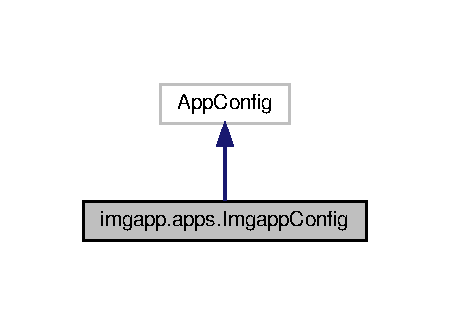
\includegraphics[width=216pt]{classimgapp_1_1apps_1_1ImgappConfig__inherit__graph}
\end{center}
\end{figure}


Collaboration diagram for imgapp.\+apps.\+Imgapp\+Config\+:\nopagebreak
\begin{figure}[H]
\begin{center}
\leavevmode
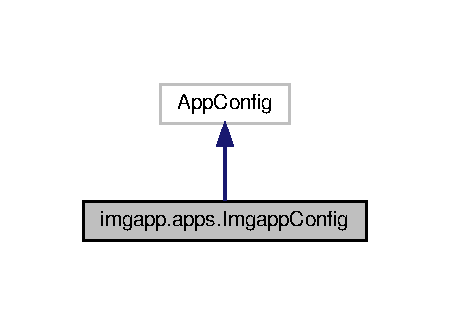
\includegraphics[width=216pt]{classimgapp_1_1apps_1_1ImgappConfig__coll__graph}
\end{center}
\end{figure}
\subsection*{Static Public Attributes}
\begin{DoxyCompactItemize}
\item 
string \hyperlink{classimgapp_1_1apps_1_1ImgappConfig_a3eafdf46b561d2f3764888b9e7cfe9e5}{name} = \textquotesingle{}imgapp\textquotesingle{}
\end{DoxyCompactItemize}


\subsection{Detailed Description}
imgapp A\+PI class 

\subsection{Member Data Documentation}
\mbox{\Hypertarget{classimgapp_1_1apps_1_1ImgappConfig_a3eafdf46b561d2f3764888b9e7cfe9e5}\label{classimgapp_1_1apps_1_1ImgappConfig_a3eafdf46b561d2f3764888b9e7cfe9e5}} 
\index{imgapp\+::apps\+::\+Imgapp\+Config@{imgapp\+::apps\+::\+Imgapp\+Config}!name@{name}}
\index{name@{name}!imgapp\+::apps\+::\+Imgapp\+Config@{imgapp\+::apps\+::\+Imgapp\+Config}}
\subsubsection{\texorpdfstring{name}{name}}
{\footnotesize\ttfamily string imgapp.\+apps.\+Imgapp\+Config.\+name = \textquotesingle{}imgapp\textquotesingle{}\hspace{0.3cm}{\ttfamily [static]}}



The documentation for this class was generated from the following file\+:\begin{DoxyCompactItemize}
\item 
imgapp/\hyperlink{apps_8py}{apps.\+py}\end{DoxyCompactItemize}

\hypertarget{classimgapp_1_1forms_1_1UserForm_1_1Meta}{}\section{imgapp.\+forms.\+User\+Form.\+Meta Class Reference}
\label{classimgapp_1_1forms_1_1UserForm_1_1Meta}\index{imgapp.\+forms.\+User\+Form.\+Meta@{imgapp.\+forms.\+User\+Form.\+Meta}}


meta class  


\subsection*{Static Public Attributes}
\begin{DoxyCompactItemize}
\item 
\hyperlink{classimgapp_1_1forms_1_1UserForm_1_1Meta_ae646e248a6bf9567c583461a2df4a836}{model} = User
\item 
tuple \hyperlink{classimgapp_1_1forms_1_1UserForm_1_1Meta_a3db99dc49ab4b8ad78e26cf780b6d276}{fields} = (\textquotesingle{}username\textquotesingle{}, \textquotesingle{}password\textquotesingle{}, \textquotesingle{}email\textquotesingle{})
\end{DoxyCompactItemize}


\subsection{Detailed Description}
meta class 

\subsection{Member Data Documentation}
\mbox{\Hypertarget{classimgapp_1_1forms_1_1UserForm_1_1Meta_a3db99dc49ab4b8ad78e26cf780b6d276}\label{classimgapp_1_1forms_1_1UserForm_1_1Meta_a3db99dc49ab4b8ad78e26cf780b6d276}} 
\index{imgapp\+::forms\+::\+User\+Form\+::\+Meta@{imgapp\+::forms\+::\+User\+Form\+::\+Meta}!fields@{fields}}
\index{fields@{fields}!imgapp\+::forms\+::\+User\+Form\+::\+Meta@{imgapp\+::forms\+::\+User\+Form\+::\+Meta}}
\subsubsection{\texorpdfstring{fields}{fields}}
{\footnotesize\ttfamily tuple imgapp.\+forms.\+User\+Form.\+Meta.\+fields = (\textquotesingle{}username\textquotesingle{}, \textquotesingle{}password\textquotesingle{}, \textquotesingle{}email\textquotesingle{})\hspace{0.3cm}{\ttfamily [static]}}

\mbox{\Hypertarget{classimgapp_1_1forms_1_1UserForm_1_1Meta_ae646e248a6bf9567c583461a2df4a836}\label{classimgapp_1_1forms_1_1UserForm_1_1Meta_ae646e248a6bf9567c583461a2df4a836}} 
\index{imgapp\+::forms\+::\+User\+Form\+::\+Meta@{imgapp\+::forms\+::\+User\+Form\+::\+Meta}!model@{model}}
\index{model@{model}!imgapp\+::forms\+::\+User\+Form\+::\+Meta@{imgapp\+::forms\+::\+User\+Form\+::\+Meta}}
\subsubsection{\texorpdfstring{model}{model}}
{\footnotesize\ttfamily imgapp.\+forms.\+User\+Form.\+Meta.\+model = User\hspace{0.3cm}{\ttfamily [static]}}



The documentation for this class was generated from the following file\+:\begin{DoxyCompactItemize}
\item 
imgapp/\hyperlink{forms_8py}{forms.\+py}\end{DoxyCompactItemize}

\hypertarget{classimgapp_1_1forms_1_1ProfileForm_1_1Meta}{}\section{imgapp.\+forms.\+Profile\+Form.\+Meta Class Reference}
\label{classimgapp_1_1forms_1_1ProfileForm_1_1Meta}\index{imgapp.\+forms.\+Profile\+Form.\+Meta@{imgapp.\+forms.\+Profile\+Form.\+Meta}}


meta class  


\subsection*{Static Public Attributes}
\begin{DoxyCompactItemize}
\item 
\hyperlink{classimgapp_1_1forms_1_1ProfileForm_1_1Meta_a1781be7cea589fabd63eec0d18cdd232}{model} = \hyperlink{classimgapp_1_1models_1_1Profile}{Profile}
\item 
tuple \hyperlink{classimgapp_1_1forms_1_1ProfileForm_1_1Meta_a30b0f2ddcde3a48b0df790c57432666e}{fields} = (\textquotesingle{}company\textquotesingle{},)
\end{DoxyCompactItemize}


\subsection{Detailed Description}
meta class 

\subsection{Member Data Documentation}
\mbox{\Hypertarget{classimgapp_1_1forms_1_1ProfileForm_1_1Meta_a30b0f2ddcde3a48b0df790c57432666e}\label{classimgapp_1_1forms_1_1ProfileForm_1_1Meta_a30b0f2ddcde3a48b0df790c57432666e}} 
\index{imgapp\+::forms\+::\+Profile\+Form\+::\+Meta@{imgapp\+::forms\+::\+Profile\+Form\+::\+Meta}!fields@{fields}}
\index{fields@{fields}!imgapp\+::forms\+::\+Profile\+Form\+::\+Meta@{imgapp\+::forms\+::\+Profile\+Form\+::\+Meta}}
\subsubsection{\texorpdfstring{fields}{fields}}
{\footnotesize\ttfamily tuple imgapp.\+forms.\+Profile\+Form.\+Meta.\+fields = (\textquotesingle{}company\textquotesingle{},)\hspace{0.3cm}{\ttfamily [static]}}

\mbox{\Hypertarget{classimgapp_1_1forms_1_1ProfileForm_1_1Meta_a1781be7cea589fabd63eec0d18cdd232}\label{classimgapp_1_1forms_1_1ProfileForm_1_1Meta_a1781be7cea589fabd63eec0d18cdd232}} 
\index{imgapp\+::forms\+::\+Profile\+Form\+::\+Meta@{imgapp\+::forms\+::\+Profile\+Form\+::\+Meta}!model@{model}}
\index{model@{model}!imgapp\+::forms\+::\+Profile\+Form\+::\+Meta@{imgapp\+::forms\+::\+Profile\+Form\+::\+Meta}}
\subsubsection{\texorpdfstring{model}{model}}
{\footnotesize\ttfamily imgapp.\+forms.\+Profile\+Form.\+Meta.\+model = \hyperlink{classimgapp_1_1models_1_1Profile}{Profile}\hspace{0.3cm}{\ttfamily [static]}}



The documentation for this class was generated from the following file\+:\begin{DoxyCompactItemize}
\item 
imgapp/\hyperlink{forms_8py}{forms.\+py}\end{DoxyCompactItemize}

\hypertarget{classimgapp_1_1migrations_1_10001__initial_1_1Migration}{}\section{imgapp.\+migrations.0001\+\_\+initial.Migration Class Reference}
\label{classimgapp_1_1migrations_1_10001__initial_1_1Migration}\index{imgapp.\+migrations.\+0001\+\_\+initial.\+Migration@{imgapp.\+migrations.\+0001\+\_\+initial.\+Migration}}


Inheritance diagram for imgapp.\+migrations.0001\+\_\+initial.Migration\+:
\nopagebreak
\begin{figure}[H]
\begin{center}
\leavevmode
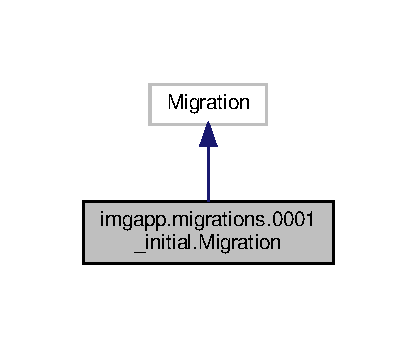
\includegraphics[width=200pt]{classimgapp_1_1migrations_1_10001__initial_1_1Migration__inherit__graph}
\end{center}
\end{figure}


Collaboration diagram for imgapp.\+migrations.0001\+\_\+initial.Migration\+:
\nopagebreak
\begin{figure}[H]
\begin{center}
\leavevmode
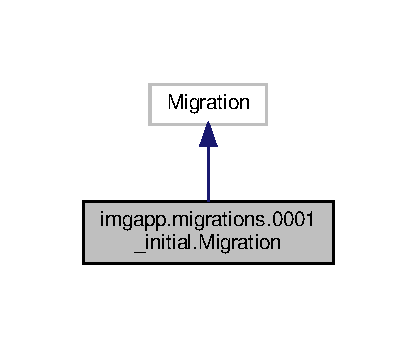
\includegraphics[width=200pt]{classimgapp_1_1migrations_1_10001__initial_1_1Migration__coll__graph}
\end{center}
\end{figure}
\subsection*{Static Public Attributes}
\begin{DoxyCompactItemize}
\item 
bool \hyperlink{classimgapp_1_1migrations_1_10001__initial_1_1Migration_a9c4795f13c3f1ba0324cabaf163417e5}{initial} = True
\item 
list \hyperlink{classimgapp_1_1migrations_1_10001__initial_1_1Migration_aa54c815fe0f4d4a5d6f1e7303a9843fc}{dependencies}
\item 
list \hyperlink{classimgapp_1_1migrations_1_10001__initial_1_1Migration_ad2e7a56581e2741b53b78c4b28663ff6}{operations}
\end{DoxyCompactItemize}


\subsection{Member Data Documentation}
\mbox{\Hypertarget{classimgapp_1_1migrations_1_10001__initial_1_1Migration_aa54c815fe0f4d4a5d6f1e7303a9843fc}\label{classimgapp_1_1migrations_1_10001__initial_1_1Migration_aa54c815fe0f4d4a5d6f1e7303a9843fc}} 
\index{imgapp\+::migrations\+::0001\+\_\+initial\+::\+Migration@{imgapp\+::migrations\+::0001\+\_\+initial\+::\+Migration}!dependencies@{dependencies}}
\index{dependencies@{dependencies}!imgapp\+::migrations\+::0001\+\_\+initial\+::\+Migration@{imgapp\+::migrations\+::0001\+\_\+initial\+::\+Migration}}
\subsubsection{\texorpdfstring{dependencies}{dependencies}}
{\footnotesize\ttfamily list imgapp.\+migrations.\+0001\+\_\+initial.\+Migration.\+dependencies\hspace{0.3cm}{\ttfamily [static]}}

{\bfseries Initial value\+:}
\begin{DoxyCode}
=  [
        migrations.swappable\_dependency(settings.AUTH\_USER\_MODEL),
    ]
\end{DoxyCode}
\mbox{\Hypertarget{classimgapp_1_1migrations_1_10001__initial_1_1Migration_a9c4795f13c3f1ba0324cabaf163417e5}\label{classimgapp_1_1migrations_1_10001__initial_1_1Migration_a9c4795f13c3f1ba0324cabaf163417e5}} 
\index{imgapp\+::migrations\+::0001\+\_\+initial\+::\+Migration@{imgapp\+::migrations\+::0001\+\_\+initial\+::\+Migration}!initial@{initial}}
\index{initial@{initial}!imgapp\+::migrations\+::0001\+\_\+initial\+::\+Migration@{imgapp\+::migrations\+::0001\+\_\+initial\+::\+Migration}}
\subsubsection{\texorpdfstring{initial}{initial}}
{\footnotesize\ttfamily bool imgapp.\+migrations.\+0001\+\_\+initial.\+Migration.\+initial = True\hspace{0.3cm}{\ttfamily [static]}}

\mbox{\Hypertarget{classimgapp_1_1migrations_1_10001__initial_1_1Migration_ad2e7a56581e2741b53b78c4b28663ff6}\label{classimgapp_1_1migrations_1_10001__initial_1_1Migration_ad2e7a56581e2741b53b78c4b28663ff6}} 
\index{imgapp\+::migrations\+::0001\+\_\+initial\+::\+Migration@{imgapp\+::migrations\+::0001\+\_\+initial\+::\+Migration}!operations@{operations}}
\index{operations@{operations}!imgapp\+::migrations\+::0001\+\_\+initial\+::\+Migration@{imgapp\+::migrations\+::0001\+\_\+initial\+::\+Migration}}
\subsubsection{\texorpdfstring{operations}{operations}}
{\footnotesize\ttfamily list imgapp.\+migrations.\+0001\+\_\+initial.\+Migration.\+operations\hspace{0.3cm}{\ttfamily [static]}}

{\bfseries Initial value\+:}
\begin{DoxyCode}
=  [
        migrations.CreateModel(
            name=\textcolor{stringliteral}{'Profile'},
            fields=[
                (\textcolor{stringliteral}{'id'}, models.AutoField(auto\_created=\textcolor{keyword}{True}, primary\_key=\textcolor{keyword}{True}, serialize=\textcolor{keyword}{False}, verbose\_name=\textcolor{stringliteral}{
      'ID'})),
                (\textcolor{stringliteral}{'company'}, models.CharField(max\_length=50)),
                (\textcolor{stringliteral}{'user'}, models.OneToOneField(on\_delete=django.db.models.deletion.CASCADE, to=
      settings.AUTH\_USER\_MODEL)),
            ],
        ),
    ]
\end{DoxyCode}


The documentation for this class was generated from the following file\+:\begin{DoxyCompactItemize}
\item 
imgapp/migrations/\hyperlink{0001__initial_8py}{0001\+\_\+initial.\+py}\end{DoxyCompactItemize}

\hypertarget{classimgapp_1_1migrations_1_10002__objects_1_1Migration}{}\section{imgapp.\+migrations.0002\+\_\+objects.Migration Class Reference}
\label{classimgapp_1_1migrations_1_10002__objects_1_1Migration}\index{imgapp.\+migrations.\+0002\+\_\+objects.\+Migration@{imgapp.\+migrations.\+0002\+\_\+objects.\+Migration}}


Inheritance diagram for imgapp.\+migrations.0002\+\_\+objects.Migration\+:\nopagebreak
\begin{figure}[H]
\begin{center}
\leavevmode
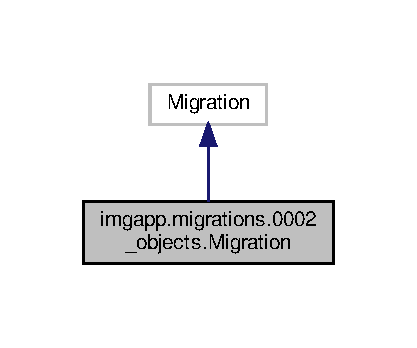
\includegraphics[width=200pt]{classimgapp_1_1migrations_1_10002__objects_1_1Migration__inherit__graph}
\end{center}
\end{figure}


Collaboration diagram for imgapp.\+migrations.0002\+\_\+objects.Migration\+:\nopagebreak
\begin{figure}[H]
\begin{center}
\leavevmode
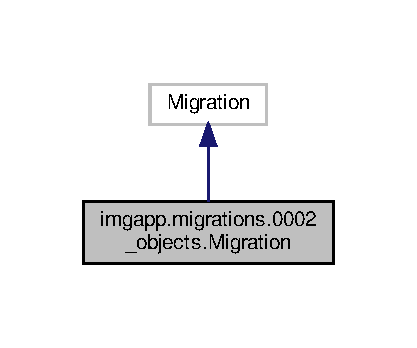
\includegraphics[width=200pt]{classimgapp_1_1migrations_1_10002__objects_1_1Migration__coll__graph}
\end{center}
\end{figure}
\subsection*{Static Public Attributes}
\begin{DoxyCompactItemize}
\item 
list \hyperlink{classimgapp_1_1migrations_1_10002__objects_1_1Migration_abd3fa170eb3a3149ee43f9acf33917b4}{dependencies}
\item 
list \hyperlink{classimgapp_1_1migrations_1_10002__objects_1_1Migration_adcbef6b10dcf430fa1e7ce7f4a9b700a}{operations}
\end{DoxyCompactItemize}


\subsection{Member Data Documentation}
\mbox{\Hypertarget{classimgapp_1_1migrations_1_10002__objects_1_1Migration_abd3fa170eb3a3149ee43f9acf33917b4}\label{classimgapp_1_1migrations_1_10002__objects_1_1Migration_abd3fa170eb3a3149ee43f9acf33917b4}} 
\index{imgapp\+::migrations\+::0002\+\_\+objects\+::\+Migration@{imgapp\+::migrations\+::0002\+\_\+objects\+::\+Migration}!dependencies@{dependencies}}
\index{dependencies@{dependencies}!imgapp\+::migrations\+::0002\+\_\+objects\+::\+Migration@{imgapp\+::migrations\+::0002\+\_\+objects\+::\+Migration}}
\subsubsection{\texorpdfstring{dependencies}{dependencies}}
{\footnotesize\ttfamily list imgapp.\+migrations.\+0002\+\_\+objects.\+Migration.\+dependencies\hspace{0.3cm}{\ttfamily [static]}}

{\bfseries Initial value\+:}
\begin{DoxyCode}
=  [
        (\textcolor{stringliteral}{'imgapp'}, \textcolor{stringliteral}{'0001\_initial'}),
    ]
\end{DoxyCode}
\mbox{\Hypertarget{classimgapp_1_1migrations_1_10002__objects_1_1Migration_adcbef6b10dcf430fa1e7ce7f4a9b700a}\label{classimgapp_1_1migrations_1_10002__objects_1_1Migration_adcbef6b10dcf430fa1e7ce7f4a9b700a}} 
\index{imgapp\+::migrations\+::0002\+\_\+objects\+::\+Migration@{imgapp\+::migrations\+::0002\+\_\+objects\+::\+Migration}!operations@{operations}}
\index{operations@{operations}!imgapp\+::migrations\+::0002\+\_\+objects\+::\+Migration@{imgapp\+::migrations\+::0002\+\_\+objects\+::\+Migration}}
\subsubsection{\texorpdfstring{operations}{operations}}
{\footnotesize\ttfamily list imgapp.\+migrations.\+0002\+\_\+objects.\+Migration.\+operations\hspace{0.3cm}{\ttfamily [static]}}

{\bfseries Initial value\+:}
\begin{DoxyCode}
=  [
        migrations.CreateModel(
            name=\textcolor{stringliteral}{'Objects'},
            fields=[
                (\textcolor{stringliteral}{'id'}, models.AutoField(auto\_created=\textcolor{keyword}{True}, primary\_key=\textcolor{keyword}{True}, serialize=\textcolor{keyword}{False}, verbose\_name=\textcolor{stringliteral}{
      'ID'})),
                (\textcolor{stringliteral}{'objectslist'}, models.CharField(max\_length=4000)),
            ],
        ),
    ]
\end{DoxyCode}


The documentation for this class was generated from the following file\+:\begin{DoxyCompactItemize}
\item 
imgapp/migrations/\hyperlink{0002__objects_8py}{0002\+\_\+objects.\+py}\end{DoxyCompactItemize}

\hypertarget{classimgapp_1_1migrations_1_10003__description_1_1Migration}{}\section{imgapp.\+migrations.0003\+\_\+description.Migration Class Reference}
\label{classimgapp_1_1migrations_1_10003__description_1_1Migration}\index{imgapp.\+migrations.\+0003\+\_\+description.\+Migration@{imgapp.\+migrations.\+0003\+\_\+description.\+Migration}}


Inheritance diagram for imgapp.\+migrations.0003\+\_\+description.Migration\+:
\nopagebreak
\begin{figure}[H]
\begin{center}
\leavevmode
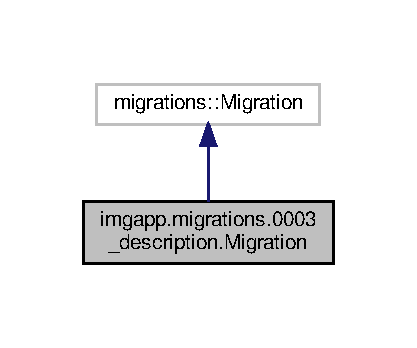
\includegraphics[width=200pt]{classimgapp_1_1migrations_1_10003__description_1_1Migration__inherit__graph}
\end{center}
\end{figure}


Collaboration diagram for imgapp.\+migrations.0003\+\_\+description.Migration\+:
\nopagebreak
\begin{figure}[H]
\begin{center}
\leavevmode
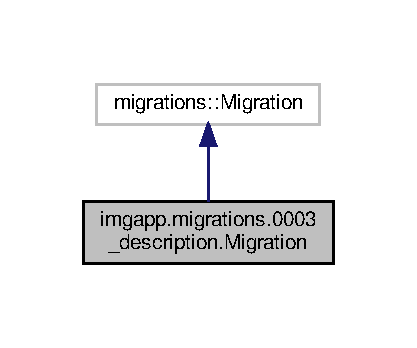
\includegraphics[width=200pt]{classimgapp_1_1migrations_1_10003__description_1_1Migration__coll__graph}
\end{center}
\end{figure}
\subsection*{Static Public Attributes}
\begin{DoxyCompactItemize}
\item 
list \hyperlink{classimgapp_1_1migrations_1_10003__description_1_1Migration_a40f33614bdb25e858eda0b1a630f42d3}{dependencies}
\item 
list \hyperlink{classimgapp_1_1migrations_1_10003__description_1_1Migration_ad23f57a54400743233700b5fe50cb6c8}{operations}
\end{DoxyCompactItemize}


\subsection{Member Data Documentation}
\mbox{\Hypertarget{classimgapp_1_1migrations_1_10003__description_1_1Migration_a40f33614bdb25e858eda0b1a630f42d3}\label{classimgapp_1_1migrations_1_10003__description_1_1Migration_a40f33614bdb25e858eda0b1a630f42d3}} 
\index{imgapp\+::migrations\+::0003\+\_\+description\+::\+Migration@{imgapp\+::migrations\+::0003\+\_\+description\+::\+Migration}!dependencies@{dependencies}}
\index{dependencies@{dependencies}!imgapp\+::migrations\+::0003\+\_\+description\+::\+Migration@{imgapp\+::migrations\+::0003\+\_\+description\+::\+Migration}}
\subsubsection{\texorpdfstring{dependencies}{dependencies}}
{\footnotesize\ttfamily list imgapp.\+migrations.\+0003\+\_\+description.\+Migration.\+dependencies\hspace{0.3cm}{\ttfamily [static]}}

{\bfseries Initial value\+:}
\begin{DoxyCode}
=  [
        (\textcolor{stringliteral}{'imgapp'}, \textcolor{stringliteral}{'0002\_objects'}),
    ]
\end{DoxyCode}
\mbox{\Hypertarget{classimgapp_1_1migrations_1_10003__description_1_1Migration_ad23f57a54400743233700b5fe50cb6c8}\label{classimgapp_1_1migrations_1_10003__description_1_1Migration_ad23f57a54400743233700b5fe50cb6c8}} 
\index{imgapp\+::migrations\+::0003\+\_\+description\+::\+Migration@{imgapp\+::migrations\+::0003\+\_\+description\+::\+Migration}!operations@{operations}}
\index{operations@{operations}!imgapp\+::migrations\+::0003\+\_\+description\+::\+Migration@{imgapp\+::migrations\+::0003\+\_\+description\+::\+Migration}}
\subsubsection{\texorpdfstring{operations}{operations}}
{\footnotesize\ttfamily list imgapp.\+migrations.\+0003\+\_\+description.\+Migration.\+operations\hspace{0.3cm}{\ttfamily [static]}}

{\bfseries Initial value\+:}
\begin{DoxyCode}
=  [
        migrations.CreateModel(
            name=\textcolor{stringliteral}{'Description'},
            fields=[
                (\textcolor{stringliteral}{'id'}, models.AutoField(auto\_created=\textcolor{keyword}{True}, primary\_key=\textcolor{keyword}{True}, serialize=\textcolor{keyword}{False}, verbose\_name=\textcolor{stringliteral}{
      'ID'})),
                (\textcolor{stringliteral}{'description'}, models.TextField(help\_text=\textcolor{stringliteral}{'Based in Silicon Valley and Indian Institute of
       Technology Delhi (IIT-Delhi), we are a group of researchers and entrepreneurs with a fondness for all
       thing’s deep tech and sci-fi.We aim to solve real world remote sensing problems through Galactica.AI platform by
       bringing the best minds in research and academia along with strategic industry partnership \(\backslash\)n Our R&D team,
       based out of IIT Delhi is building the core Artificial Intelligence & Machine Learning software
       infrastructure that can be applied for all the verticals mentioned. Our core software infrastructure is capable of
       analysing large amounts of video data and doing operations including map generation, orthorectification,
       photogrammetry, object detection, object tracking, change detection & more. \(\backslash\)n Instead of building a
       one-size-fits-all solution, our team will work closely with customers to customise the Galactica.AI platform to build a
       solution that works closely with the available infrastructure of the client to deliver very specific needs. Our
       goal is to reduce barrier to adoption by creating a seamless transition to our platform.'})),
            ],
        ),
    ]
\end{DoxyCode}


The documentation for this class was generated from the following file\+:\begin{DoxyCompactItemize}
\item 
imgapp/migrations/\hyperlink{0003__description_8py}{0003\+\_\+description.\+py}\end{DoxyCompactItemize}

\hypertarget{classimgapp_1_1migrations_1_10004__auto__20190715__1327_1_1Migration}{}\section{imgapp.\+migrations.0004\+\_\+auto\+\_\+20190715\+\_\+1327.Migration Class Reference}
\label{classimgapp_1_1migrations_1_10004__auto__20190715__1327_1_1Migration}\index{imgapp.\+migrations.\+0004\+\_\+auto\+\_\+20190715\+\_\+1327.\+Migration@{imgapp.\+migrations.\+0004\+\_\+auto\+\_\+20190715\+\_\+1327.\+Migration}}


Inheritance diagram for imgapp.\+migrations.0004\+\_\+auto\+\_\+20190715\+\_\+1327.Migration\+:
\nopagebreak
\begin{figure}[H]
\begin{center}
\leavevmode
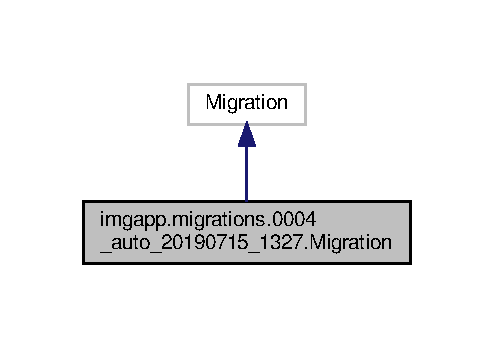
\includegraphics[width=237pt]{classimgapp_1_1migrations_1_10004__auto__20190715__1327_1_1Migration__inherit__graph}
\end{center}
\end{figure}


Collaboration diagram for imgapp.\+migrations.0004\+\_\+auto\+\_\+20190715\+\_\+1327.Migration\+:
\nopagebreak
\begin{figure}[H]
\begin{center}
\leavevmode
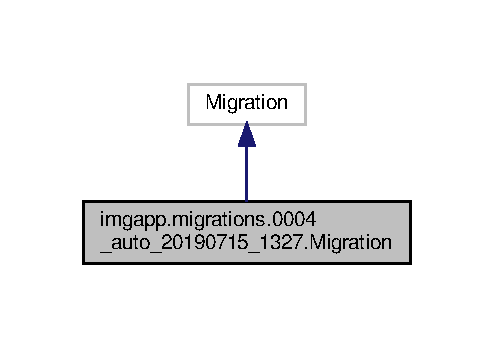
\includegraphics[width=237pt]{classimgapp_1_1migrations_1_10004__auto__20190715__1327_1_1Migration__coll__graph}
\end{center}
\end{figure}
\subsection*{Static Public Attributes}
\begin{DoxyCompactItemize}
\item 
list \hyperlink{classimgapp_1_1migrations_1_10004__auto__20190715__1327_1_1Migration_af829ee09f3fc357512f148fb26db4e13}{dependencies}
\item 
list \hyperlink{classimgapp_1_1migrations_1_10004__auto__20190715__1327_1_1Migration_aef8338a6773cec3d5822a44bcdef9738}{operations}
\end{DoxyCompactItemize}


\subsection{Member Data Documentation}
\mbox{\Hypertarget{classimgapp_1_1migrations_1_10004__auto__20190715__1327_1_1Migration_af829ee09f3fc357512f148fb26db4e13}\label{classimgapp_1_1migrations_1_10004__auto__20190715__1327_1_1Migration_af829ee09f3fc357512f148fb26db4e13}} 
\index{imgapp\+::migrations\+::0004\+\_\+auto\+\_\+20190715\+\_\+1327\+::\+Migration@{imgapp\+::migrations\+::0004\+\_\+auto\+\_\+20190715\+\_\+1327\+::\+Migration}!dependencies@{dependencies}}
\index{dependencies@{dependencies}!imgapp\+::migrations\+::0004\+\_\+auto\+\_\+20190715\+\_\+1327\+::\+Migration@{imgapp\+::migrations\+::0004\+\_\+auto\+\_\+20190715\+\_\+1327\+::\+Migration}}
\subsubsection{\texorpdfstring{dependencies}{dependencies}}
{\footnotesize\ttfamily list imgapp.\+migrations.\+0004\+\_\+auto\+\_\+20190715\+\_\+1327.\+Migration.\+dependencies\hspace{0.3cm}{\ttfamily [static]}}

{\bfseries Initial value\+:}
\begin{DoxyCode}
=  [
        (\textcolor{stringliteral}{'imgapp'}, \textcolor{stringliteral}{'0003\_description'}),
    ]
\end{DoxyCode}
\mbox{\Hypertarget{classimgapp_1_1migrations_1_10004__auto__20190715__1327_1_1Migration_aef8338a6773cec3d5822a44bcdef9738}\label{classimgapp_1_1migrations_1_10004__auto__20190715__1327_1_1Migration_aef8338a6773cec3d5822a44bcdef9738}} 
\index{imgapp\+::migrations\+::0004\+\_\+auto\+\_\+20190715\+\_\+1327\+::\+Migration@{imgapp\+::migrations\+::0004\+\_\+auto\+\_\+20190715\+\_\+1327\+::\+Migration}!operations@{operations}}
\index{operations@{operations}!imgapp\+::migrations\+::0004\+\_\+auto\+\_\+20190715\+\_\+1327\+::\+Migration@{imgapp\+::migrations\+::0004\+\_\+auto\+\_\+20190715\+\_\+1327\+::\+Migration}}
\subsubsection{\texorpdfstring{operations}{operations}}
{\footnotesize\ttfamily list imgapp.\+migrations.\+0004\+\_\+auto\+\_\+20190715\+\_\+1327.\+Migration.\+operations\hspace{0.3cm}{\ttfamily [static]}}

{\bfseries Initial value\+:}
\begin{DoxyCode}
=  [
        migrations.DeleteModel(
            name=\textcolor{stringliteral}{'Description'},
        ),
        migrations.DeleteModel(
            name=\textcolor{stringliteral}{'Objects'},
        ),
    ]
\end{DoxyCode}


The documentation for this class was generated from the following file\+:\begin{DoxyCompactItemize}
\item 
imgapp/migrations/\hyperlink{0004__auto__20190715__1327_8py}{0004\+\_\+auto\+\_\+20190715\+\_\+1327.\+py}\end{DoxyCompactItemize}

\hypertarget{classimgapp_1_1MongoQuery_1_1mongoQuery}{}\section{imgapp.\+Mongo\+Query.\+mongo\+Query Class Reference}
\label{classimgapp_1_1MongoQuery_1_1mongoQuery}\index{imgapp.\+Mongo\+Query.\+mongo\+Query@{imgapp.\+Mongo\+Query.\+mongo\+Query}}


Class to query mongo\+DB.  


\subsection*{Public Member Functions}
\begin{DoxyCompactItemize}
\item 
def \hyperlink{classimgapp_1_1MongoQuery_1_1mongoQuery_a479f815a109cb18629f60c824a05ca3d}{\+\_\+\+\_\+init\+\_\+\+\_\+} (self)
\begin{DoxyCompactList}\small\item\em constructor \end{DoxyCompactList}\item 
def \hyperlink{classimgapp_1_1MongoQuery_1_1mongoQuery_a34be40a7a016956c3e956559f800a083}{find\+\_\+key} (self, queryfield, Config)
\begin{DoxyCompactList}\small\item\em find the super-\/class from the object class name \end{DoxyCompactList}\item 
def \hyperlink{classimgapp_1_1MongoQuery_1_1mongoQuery_a475c6a422417c03491d71648dbd97caa}{custom\+\_\+search} (self, Query\+Value, user\+ID, searchtype, create\+\_\+start, create\+\_\+till)
\begin{DoxyCompactList}\small\item\em return images satisfying the query in the user\textquotesingle{}s own mongo collection \end{DoxyCompactList}\item 
def \hyperlink{classimgapp_1_1MongoQuery_1_1mongoQuery_a1936fd6102804ca6e33dd26a3dacab2c}{Find\+Objects\+C\+O\+CO} (self, Query\+Value)
\begin{DoxyCompactList}\small\item\em find coco images with queried images \end{DoxyCompactList}\end{DoxyCompactItemize}
\subsection*{Public Attributes}
\begin{DoxyCompactItemize}
\item 
\hyperlink{classimgapp_1_1MongoQuery_1_1mongoQuery_a6f032a87b0cbdd86d27cb57bdb56d177}{timestamps\+C\+Ol}
\item 
\hyperlink{classimgapp_1_1MongoQuery_1_1mongoQuery_a1c2a13999b3db775d7135512c5c56af5}{settings}
\item 
\hyperlink{classimgapp_1_1MongoQuery_1_1mongoQuery_a841c5742f5a879b1fac81cd85d0bd6d3}{classes}
\end{DoxyCompactItemize}
\subsection*{Static Public Attributes}
\begin{DoxyCompactItemize}
\item 
\hyperlink{classimgapp_1_1MongoQuery_1_1mongoQuery_a1cdb54173fb250f4713191aa1a146d4e}{client} = None
\begin{DoxyCompactList}\small\item\em Mongo Client. \end{DoxyCompactList}\item 
\hyperlink{classimgapp_1_1MongoQuery_1_1mongoQuery_a175902875f9b19da7484777c2d76386a}{db} = None
\begin{DoxyCompactList}\small\item\em Datatbase containing collection of meta-\/data of images. \end{DoxyCompactList}\item 
\hyperlink{classimgapp_1_1MongoQuery_1_1mongoQuery_a4706154c37ca22643d084e3903f11240}{Col} = None
\begin{DoxyCompactList}\small\item\em Collection, each user has a different collection. \end{DoxyCompactList}\end{DoxyCompactItemize}


\subsection{Detailed Description}
Class to query mongo\+DB. 

Query on documents in Mongo\+DB 

\subsection{Constructor \& Destructor Documentation}
\mbox{\Hypertarget{classimgapp_1_1MongoQuery_1_1mongoQuery_a479f815a109cb18629f60c824a05ca3d}\label{classimgapp_1_1MongoQuery_1_1mongoQuery_a479f815a109cb18629f60c824a05ca3d}} 
\index{imgapp\+::\+Mongo\+Query\+::mongo\+Query@{imgapp\+::\+Mongo\+Query\+::mongo\+Query}!\+\_\+\+\_\+init\+\_\+\+\_\+@{\+\_\+\+\_\+init\+\_\+\+\_\+}}
\index{\+\_\+\+\_\+init\+\_\+\+\_\+@{\+\_\+\+\_\+init\+\_\+\+\_\+}!imgapp\+::\+Mongo\+Query\+::mongo\+Query@{imgapp\+::\+Mongo\+Query\+::mongo\+Query}}
\subsubsection{\texorpdfstring{\+\_\+\+\_\+init\+\_\+\+\_\+()}{\_\_init\_\_()}}
{\footnotesize\ttfamily def imgapp.\+Mongo\+Query.\+mongo\+Query.\+\_\+\+\_\+init\+\_\+\+\_\+ (\begin{DoxyParamCaption}\item[{}]{self }\end{DoxyParamCaption})}



constructor 


\begin{DoxyParams}{Parameters}
{\em self} & reference to it\textquotesingle{}s own object \\
\hline
\end{DoxyParams}


\subsection{Member Function Documentation}
\mbox{\Hypertarget{classimgapp_1_1MongoQuery_1_1mongoQuery_a475c6a422417c03491d71648dbd97caa}\label{classimgapp_1_1MongoQuery_1_1mongoQuery_a475c6a422417c03491d71648dbd97caa}} 
\index{imgapp\+::\+Mongo\+Query\+::mongo\+Query@{imgapp\+::\+Mongo\+Query\+::mongo\+Query}!custom\+\_\+search@{custom\+\_\+search}}
\index{custom\+\_\+search@{custom\+\_\+search}!imgapp\+::\+Mongo\+Query\+::mongo\+Query@{imgapp\+::\+Mongo\+Query\+::mongo\+Query}}
\subsubsection{\texorpdfstring{custom\+\_\+search()}{custom\_search()}}
{\footnotesize\ttfamily def imgapp.\+Mongo\+Query.\+mongo\+Query.\+custom\+\_\+search (\begin{DoxyParamCaption}\item[{}]{self,  }\item[{}]{Query\+Value,  }\item[{}]{user\+ID,  }\item[{}]{searchtype,  }\item[{}]{create\+\_\+start,  }\item[{}]{create\+\_\+till }\end{DoxyParamCaption})}



return images satisfying the query in the user\textquotesingle{}s own mongo collection 


\begin{DoxyParams}{Parameters}
{\em self} & reference to it\textquotesingle{}s own object \\
\hline
{\em Query\+Value} & objects list in the query \\
\hline
{\em user\+ID} & primary key of the user model instance \\
\hline
{\em searchtype} & check whether to query on images uploaded lastime or all the images uploaded till now \\
\hline
{\em create\+\_\+start} & lowerlimit of the timestamp when the image was created \\
\hline
{\em create\+\_\+till} & upperlimit of the timestamp when the image was created \\
\hline
\end{DoxyParams}
\mbox{\Hypertarget{classimgapp_1_1MongoQuery_1_1mongoQuery_a34be40a7a016956c3e956559f800a083}\label{classimgapp_1_1MongoQuery_1_1mongoQuery_a34be40a7a016956c3e956559f800a083}} 
\index{imgapp\+::\+Mongo\+Query\+::mongo\+Query@{imgapp\+::\+Mongo\+Query\+::mongo\+Query}!find\+\_\+key@{find\+\_\+key}}
\index{find\+\_\+key@{find\+\_\+key}!imgapp\+::\+Mongo\+Query\+::mongo\+Query@{imgapp\+::\+Mongo\+Query\+::mongo\+Query}}
\subsubsection{\texorpdfstring{find\+\_\+key()}{find\_key()}}
{\footnotesize\ttfamily def imgapp.\+Mongo\+Query.\+mongo\+Query.\+find\+\_\+key (\begin{DoxyParamCaption}\item[{}]{self,  }\item[{}]{queryfield,  }\item[{}]{Config }\end{DoxyParamCaption})}



find the super-\/class from the object class name 


\begin{DoxyParams}{Parameters}
{\em self} & reference to it\textquotesingle{}s own object \\
\hline
{\em queryfield} & object class name \\
\hline
{\em Config} & dictionary with superclass and object mapping \\
\hline
\end{DoxyParams}
\mbox{\Hypertarget{classimgapp_1_1MongoQuery_1_1mongoQuery_a1936fd6102804ca6e33dd26a3dacab2c}\label{classimgapp_1_1MongoQuery_1_1mongoQuery_a1936fd6102804ca6e33dd26a3dacab2c}} 
\index{imgapp\+::\+Mongo\+Query\+::mongo\+Query@{imgapp\+::\+Mongo\+Query\+::mongo\+Query}!Find\+Objects\+C\+O\+CO@{Find\+Objects\+C\+O\+CO}}
\index{Find\+Objects\+C\+O\+CO@{Find\+Objects\+C\+O\+CO}!imgapp\+::\+Mongo\+Query\+::mongo\+Query@{imgapp\+::\+Mongo\+Query\+::mongo\+Query}}
\subsubsection{\texorpdfstring{Find\+Objects\+C\+O\+C\+O()}{FindObjectsCOCO()}}
{\footnotesize\ttfamily def imgapp.\+Mongo\+Query.\+mongo\+Query.\+Find\+Objects\+C\+O\+CO (\begin{DoxyParamCaption}\item[{}]{self,  }\item[{}]{Query\+Value }\end{DoxyParamCaption})}



find coco images with queried images 


\begin{DoxyParams}{Parameters}
{\em self} & reference to it\textquotesingle{}s own object \\
\hline
{\em Query\+Value} & list of objects in the query \\
\hline
\end{DoxyParams}


\subsection{Member Data Documentation}
\mbox{\Hypertarget{classimgapp_1_1MongoQuery_1_1mongoQuery_a841c5742f5a879b1fac81cd85d0bd6d3}\label{classimgapp_1_1MongoQuery_1_1mongoQuery_a841c5742f5a879b1fac81cd85d0bd6d3}} 
\index{imgapp\+::\+Mongo\+Query\+::mongo\+Query@{imgapp\+::\+Mongo\+Query\+::mongo\+Query}!classes@{classes}}
\index{classes@{classes}!imgapp\+::\+Mongo\+Query\+::mongo\+Query@{imgapp\+::\+Mongo\+Query\+::mongo\+Query}}
\subsubsection{\texorpdfstring{classes}{classes}}
{\footnotesize\ttfamily imgapp.\+Mongo\+Query.\+mongo\+Query.\+classes}

\mbox{\Hypertarget{classimgapp_1_1MongoQuery_1_1mongoQuery_a1cdb54173fb250f4713191aa1a146d4e}\label{classimgapp_1_1MongoQuery_1_1mongoQuery_a1cdb54173fb250f4713191aa1a146d4e}} 
\index{imgapp\+::\+Mongo\+Query\+::mongo\+Query@{imgapp\+::\+Mongo\+Query\+::mongo\+Query}!client@{client}}
\index{client@{client}!imgapp\+::\+Mongo\+Query\+::mongo\+Query@{imgapp\+::\+Mongo\+Query\+::mongo\+Query}}
\subsubsection{\texorpdfstring{client}{client}}
{\footnotesize\ttfamily imgapp.\+Mongo\+Query.\+mongo\+Query.\+client = None\hspace{0.3cm}{\ttfamily [static]}}



Mongo Client. 

\mbox{\Hypertarget{classimgapp_1_1MongoQuery_1_1mongoQuery_a4706154c37ca22643d084e3903f11240}\label{classimgapp_1_1MongoQuery_1_1mongoQuery_a4706154c37ca22643d084e3903f11240}} 
\index{imgapp\+::\+Mongo\+Query\+::mongo\+Query@{imgapp\+::\+Mongo\+Query\+::mongo\+Query}!Col@{Col}}
\index{Col@{Col}!imgapp\+::\+Mongo\+Query\+::mongo\+Query@{imgapp\+::\+Mongo\+Query\+::mongo\+Query}}
\subsubsection{\texorpdfstring{Col}{Col}}
{\footnotesize\ttfamily imgapp.\+Mongo\+Query.\+mongo\+Query.\+Col = None\hspace{0.3cm}{\ttfamily [static]}}



Collection, each user has a different collection. 

\mbox{\Hypertarget{classimgapp_1_1MongoQuery_1_1mongoQuery_a175902875f9b19da7484777c2d76386a}\label{classimgapp_1_1MongoQuery_1_1mongoQuery_a175902875f9b19da7484777c2d76386a}} 
\index{imgapp\+::\+Mongo\+Query\+::mongo\+Query@{imgapp\+::\+Mongo\+Query\+::mongo\+Query}!db@{db}}
\index{db@{db}!imgapp\+::\+Mongo\+Query\+::mongo\+Query@{imgapp\+::\+Mongo\+Query\+::mongo\+Query}}
\subsubsection{\texorpdfstring{db}{db}}
{\footnotesize\ttfamily imgapp.\+Mongo\+Query.\+mongo\+Query.\+db = None\hspace{0.3cm}{\ttfamily [static]}}



Datatbase containing collection of meta-\/data of images. 

\mbox{\Hypertarget{classimgapp_1_1MongoQuery_1_1mongoQuery_a1c2a13999b3db775d7135512c5c56af5}\label{classimgapp_1_1MongoQuery_1_1mongoQuery_a1c2a13999b3db775d7135512c5c56af5}} 
\index{imgapp\+::\+Mongo\+Query\+::mongo\+Query@{imgapp\+::\+Mongo\+Query\+::mongo\+Query}!settings@{settings}}
\index{settings@{settings}!imgapp\+::\+Mongo\+Query\+::mongo\+Query@{imgapp\+::\+Mongo\+Query\+::mongo\+Query}}
\subsubsection{\texorpdfstring{settings}{settings}}
{\footnotesize\ttfamily imgapp.\+Mongo\+Query.\+mongo\+Query.\+settings}

\mbox{\Hypertarget{classimgapp_1_1MongoQuery_1_1mongoQuery_a6f032a87b0cbdd86d27cb57bdb56d177}\label{classimgapp_1_1MongoQuery_1_1mongoQuery_a6f032a87b0cbdd86d27cb57bdb56d177}} 
\index{imgapp\+::\+Mongo\+Query\+::mongo\+Query@{imgapp\+::\+Mongo\+Query\+::mongo\+Query}!timestamps\+C\+Ol@{timestamps\+C\+Ol}}
\index{timestamps\+C\+Ol@{timestamps\+C\+Ol}!imgapp\+::\+Mongo\+Query\+::mongo\+Query@{imgapp\+::\+Mongo\+Query\+::mongo\+Query}}
\subsubsection{\texorpdfstring{timestamps\+C\+Ol}{timestampsCOl}}
{\footnotesize\ttfamily imgapp.\+Mongo\+Query.\+mongo\+Query.\+timestamps\+C\+Ol}



The documentation for this class was generated from the following file\+:\begin{DoxyCompactItemize}
\item 
imgapp/\hyperlink{MongoQuery_8py}{Mongo\+Query.\+py}\end{DoxyCompactItemize}

\hypertarget{classimgapp_1_1models_1_1Profile}{}\section{imgapp.\+models.\+Profile Class Reference}
\label{classimgapp_1_1models_1_1Profile}\index{imgapp.\+models.\+Profile@{imgapp.\+models.\+Profile}}


User \hyperlink{classimgapp_1_1models_1_1Profile}{Profile}.  




Inheritance diagram for imgapp.\+models.\+Profile\+:\nopagebreak
\begin{figure}[H]
\begin{center}
\leavevmode
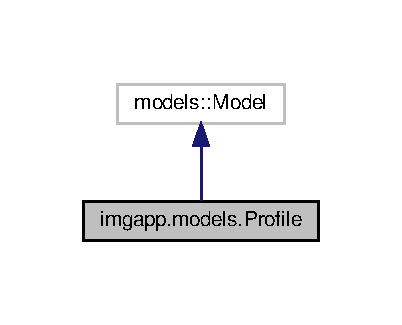
\includegraphics[width=193pt]{classimgapp_1_1models_1_1Profile__inherit__graph}
\end{center}
\end{figure}


Collaboration diagram for imgapp.\+models.\+Profile\+:\nopagebreak
\begin{figure}[H]
\begin{center}
\leavevmode
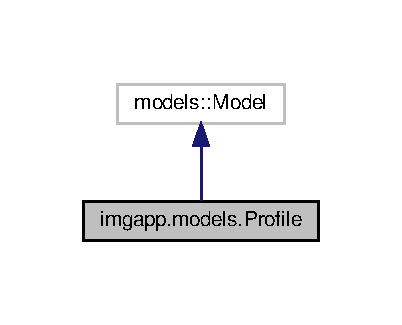
\includegraphics[width=193pt]{classimgapp_1_1models_1_1Profile__coll__graph}
\end{center}
\end{figure}
\subsection*{Static Public Attributes}
\begin{DoxyCompactItemize}
\item 
\hyperlink{classimgapp_1_1models_1_1Profile_a42a93bae8e707591dbd2eea4f5f2cb28}{user} = models.\+One\+To\+One\+Field(User,on\+\_\+delete=models.\+C\+A\+S\+C\+A\+DE)
\item 
\hyperlink{classimgapp_1_1models_1_1Profile_a7204f3b8cc0278caf80fab184397f7ae}{company} = models.\+Char\+Field(max\+\_\+length=50)
\end{DoxyCompactItemize}


\subsection{Detailed Description}
User \hyperlink{classimgapp_1_1models_1_1Profile}{Profile}. 

One to One reationship with the Django User model. So, the fields of the User models can be used direclty.~\newline
 Can add extra model fields if needed. 

\subsection{Member Data Documentation}
\mbox{\Hypertarget{classimgapp_1_1models_1_1Profile_a7204f3b8cc0278caf80fab184397f7ae}\label{classimgapp_1_1models_1_1Profile_a7204f3b8cc0278caf80fab184397f7ae}} 
\index{imgapp\+::models\+::\+Profile@{imgapp\+::models\+::\+Profile}!company@{company}}
\index{company@{company}!imgapp\+::models\+::\+Profile@{imgapp\+::models\+::\+Profile}}
\subsubsection{\texorpdfstring{company}{company}}
{\footnotesize\ttfamily imgapp.\+models.\+Profile.\+company = models.\+Char\+Field(max\+\_\+length=50)\hspace{0.3cm}{\ttfamily [static]}}

\mbox{\Hypertarget{classimgapp_1_1models_1_1Profile_a42a93bae8e707591dbd2eea4f5f2cb28}\label{classimgapp_1_1models_1_1Profile_a42a93bae8e707591dbd2eea4f5f2cb28}} 
\index{imgapp\+::models\+::\+Profile@{imgapp\+::models\+::\+Profile}!user@{user}}
\index{user@{user}!imgapp\+::models\+::\+Profile@{imgapp\+::models\+::\+Profile}}
\subsubsection{\texorpdfstring{user}{user}}
{\footnotesize\ttfamily imgapp.\+models.\+Profile.\+user = models.\+One\+To\+One\+Field(User,on\+\_\+delete=models.\+C\+A\+S\+C\+A\+DE)\hspace{0.3cm}{\ttfamily [static]}}



The documentation for this class was generated from the following file\+:\begin{DoxyCompactItemize}
\item 
imgapp/\hyperlink{models_8py}{models.\+py}\end{DoxyCompactItemize}

\hypertarget{classimgapp_1_1forms_1_1ProfileForm}{}\section{imgapp.\+forms.\+Profile\+Form Class Reference}
\label{classimgapp_1_1forms_1_1ProfileForm}\index{imgapp.\+forms.\+Profile\+Form@{imgapp.\+forms.\+Profile\+Form}}


\hyperlink{classimgapp_1_1forms_1_1ProfileForm}{Profile\+Form}.  




Inheritance diagram for imgapp.\+forms.\+Profile\+Form\+:
\nopagebreak
\begin{figure}[H]
\begin{center}
\leavevmode
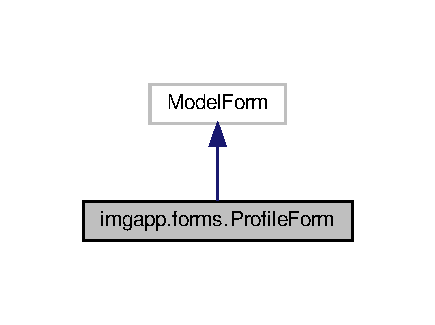
\includegraphics[width=209pt]{classimgapp_1_1forms_1_1ProfileForm__inherit__graph}
\end{center}
\end{figure}


Collaboration diagram for imgapp.\+forms.\+Profile\+Form\+:
\nopagebreak
\begin{figure}[H]
\begin{center}
\leavevmode
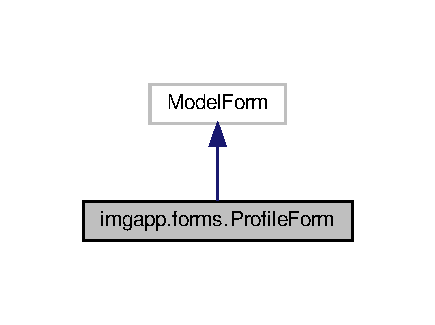
\includegraphics[width=209pt]{classimgapp_1_1forms_1_1ProfileForm__coll__graph}
\end{center}
\end{figure}
\subsection*{Classes}
\begin{DoxyCompactItemize}
\item 
class \hyperlink{classimgapp_1_1forms_1_1ProfileForm_1_1Meta}{Meta}
\begin{DoxyCompactList}\small\item\em meta class \end{DoxyCompactList}\end{DoxyCompactItemize}


\subsection{Detailed Description}
\hyperlink{classimgapp_1_1forms_1_1ProfileForm}{Profile\+Form}. 

Extends Model\+Form.~\newline
 Uses the Profile Model in the \hyperlink{models_8py}{models.\+py} module.~\newline
 Form fields are company name.~\newline
 Can be used to add extra fields that are not in the Django User model.~\newline
 Used in Sign Up form. 

The documentation for this class was generated from the following file\+:\begin{DoxyCompactItemize}
\item 
imgapp/\hyperlink{forms_8py}{forms.\+py}\end{DoxyCompactItemize}

\hypertarget{classimgapp_1_1uploadThreadClass_1_1updateMongoThread}{}\section{imgapp.\+upload\+Thread\+Class.\+update\+Mongo\+Thread Class Reference}
\label{classimgapp_1_1uploadThreadClass_1_1updateMongoThread}\index{imgapp.\+upload\+Thread\+Class.\+update\+Mongo\+Thread@{imgapp.\+upload\+Thread\+Class.\+update\+Mongo\+Thread}}


Class to update mongo\+DB.  




Inheritance diagram for imgapp.\+upload\+Thread\+Class.\+update\+Mongo\+Thread\+:
\nopagebreak
\begin{figure}[H]
\begin{center}
\leavevmode
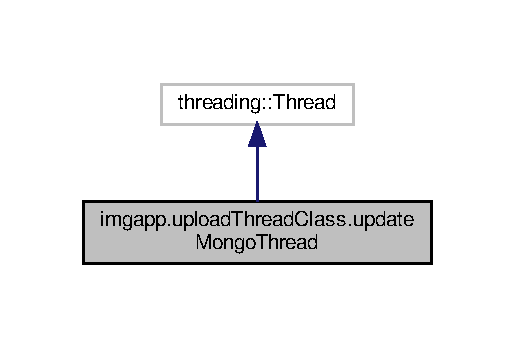
\includegraphics[width=247pt]{classimgapp_1_1uploadThreadClass_1_1updateMongoThread__inherit__graph}
\end{center}
\end{figure}


Collaboration diagram for imgapp.\+upload\+Thread\+Class.\+update\+Mongo\+Thread\+:
\nopagebreak
\begin{figure}[H]
\begin{center}
\leavevmode
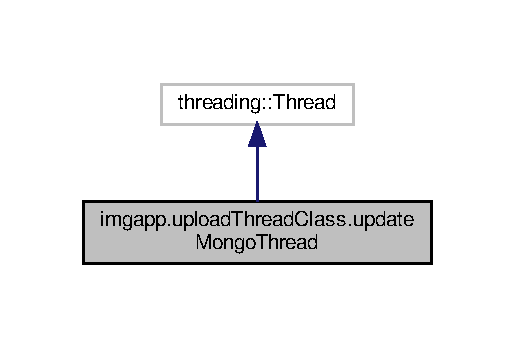
\includegraphics[width=247pt]{classimgapp_1_1uploadThreadClass_1_1updateMongoThread__coll__graph}
\end{center}
\end{figure}
\subsection*{Public Member Functions}
\begin{DoxyCompactItemize}
\item 
def \hyperlink{classimgapp_1_1uploadThreadClass_1_1updateMongoThread_aa2c07660d640e0dc5ce578df3ffcdf45}{\+\_\+\+\_\+init\+\_\+\+\_\+} (self, \hyperlink{classimgapp_1_1uploadThreadClass_1_1updateMongoThread_a7fad32b88c70b7f982c99b446776ad18}{imagetype}, \hyperlink{classimgapp_1_1uploadThreadClass_1_1updateMongoThread_a91aacecb1f2ae4f805f5d305235a365b}{path\+\_\+imagetype}, \hyperlink{classimgapp_1_1uploadThreadClass_1_1updateMongoThread_a81aeee9e6b727e234fbb83bcab0ec5db}{timestamp}, \hyperlink{classimgapp_1_1uploadThreadClass_1_1updateMongoThread_abb90747f1507aa83ad39ae4353cc7879}{user\+ID})
\begin{DoxyCompactList}\small\item\em constructor \end{DoxyCompactList}\item 
def \hyperlink{classimgapp_1_1uploadThreadClass_1_1updateMongoThread_a6f7cbd858ca77bc15b32adae2923438b}{run} (self)
\begin{DoxyCompactList}\small\item\em run method \end{DoxyCompactList}\end{DoxyCompactItemize}
\subsection*{Public Attributes}
\begin{DoxyCompactItemize}
\item 
\hyperlink{classimgapp_1_1uploadThreadClass_1_1updateMongoThread_a7fad32b88c70b7f982c99b446776ad18}{imagetype}
\item 
\hyperlink{classimgapp_1_1uploadThreadClass_1_1updateMongoThread_a91aacecb1f2ae4f805f5d305235a365b}{path\+\_\+imagetype}
\item 
\hyperlink{classimgapp_1_1uploadThreadClass_1_1updateMongoThread_a81aeee9e6b727e234fbb83bcab0ec5db}{timestamp}
\item 
\hyperlink{classimgapp_1_1uploadThreadClass_1_1updateMongoThread_abb90747f1507aa83ad39ae4353cc7879}{user\+ID}
\end{DoxyCompactItemize}


\subsection{Detailed Description}
Class to update mongo\+DB. 

thread class 

\subsection{Constructor \& Destructor Documentation}
\mbox{\Hypertarget{classimgapp_1_1uploadThreadClass_1_1updateMongoThread_aa2c07660d640e0dc5ce578df3ffcdf45}\label{classimgapp_1_1uploadThreadClass_1_1updateMongoThread_aa2c07660d640e0dc5ce578df3ffcdf45}} 
\index{imgapp\+::upload\+Thread\+Class\+::update\+Mongo\+Thread@{imgapp\+::upload\+Thread\+Class\+::update\+Mongo\+Thread}!\+\_\+\+\_\+init\+\_\+\+\_\+@{\+\_\+\+\_\+init\+\_\+\+\_\+}}
\index{\+\_\+\+\_\+init\+\_\+\+\_\+@{\+\_\+\+\_\+init\+\_\+\+\_\+}!imgapp\+::upload\+Thread\+Class\+::update\+Mongo\+Thread@{imgapp\+::upload\+Thread\+Class\+::update\+Mongo\+Thread}}
\subsubsection{\texorpdfstring{\+\_\+\+\_\+init\+\_\+\+\_\+()}{\_\_init\_\_()}}
{\footnotesize\ttfamily def imgapp.\+upload\+Thread\+Class.\+update\+Mongo\+Thread.\+\_\+\+\_\+init\+\_\+\+\_\+ (\begin{DoxyParamCaption}\item[{}]{self,  }\item[{}]{imagetype,  }\item[{}]{path\+\_\+imagetype,  }\item[{}]{timestamp,  }\item[{}]{user\+ID }\end{DoxyParamCaption})}



constructor 


\begin{DoxyParams}{Parameters}
{\em self} & reference to object itself \\
\hline
{\em imagetype} & aerial, satelite, general, etc \\
\hline
{\em timestamp} & upload timestamp \\
\hline
{\em user\+ID} & primary key of the user \\
\hline
\end{DoxyParams}


\subsection{Member Function Documentation}
\mbox{\Hypertarget{classimgapp_1_1uploadThreadClass_1_1updateMongoThread_a6f7cbd858ca77bc15b32adae2923438b}\label{classimgapp_1_1uploadThreadClass_1_1updateMongoThread_a6f7cbd858ca77bc15b32adae2923438b}} 
\index{imgapp\+::upload\+Thread\+Class\+::update\+Mongo\+Thread@{imgapp\+::upload\+Thread\+Class\+::update\+Mongo\+Thread}!run@{run}}
\index{run@{run}!imgapp\+::upload\+Thread\+Class\+::update\+Mongo\+Thread@{imgapp\+::upload\+Thread\+Class\+::update\+Mongo\+Thread}}
\subsubsection{\texorpdfstring{run()}{run()}}
{\footnotesize\ttfamily def imgapp.\+upload\+Thread\+Class.\+update\+Mongo\+Thread.\+run (\begin{DoxyParamCaption}\item[{}]{self }\end{DoxyParamCaption})}



run method 


\begin{DoxyParams}{Parameters}
{\em self} & reference to the object itself \\
\hline
\end{DoxyParams}


\subsection{Member Data Documentation}
\mbox{\Hypertarget{classimgapp_1_1uploadThreadClass_1_1updateMongoThread_a7fad32b88c70b7f982c99b446776ad18}\label{classimgapp_1_1uploadThreadClass_1_1updateMongoThread_a7fad32b88c70b7f982c99b446776ad18}} 
\index{imgapp\+::upload\+Thread\+Class\+::update\+Mongo\+Thread@{imgapp\+::upload\+Thread\+Class\+::update\+Mongo\+Thread}!imagetype@{imagetype}}
\index{imagetype@{imagetype}!imgapp\+::upload\+Thread\+Class\+::update\+Mongo\+Thread@{imgapp\+::upload\+Thread\+Class\+::update\+Mongo\+Thread}}
\subsubsection{\texorpdfstring{imagetype}{imagetype}}
{\footnotesize\ttfamily imgapp.\+upload\+Thread\+Class.\+update\+Mongo\+Thread.\+imagetype}

\mbox{\Hypertarget{classimgapp_1_1uploadThreadClass_1_1updateMongoThread_a91aacecb1f2ae4f805f5d305235a365b}\label{classimgapp_1_1uploadThreadClass_1_1updateMongoThread_a91aacecb1f2ae4f805f5d305235a365b}} 
\index{imgapp\+::upload\+Thread\+Class\+::update\+Mongo\+Thread@{imgapp\+::upload\+Thread\+Class\+::update\+Mongo\+Thread}!path\+\_\+imagetype@{path\+\_\+imagetype}}
\index{path\+\_\+imagetype@{path\+\_\+imagetype}!imgapp\+::upload\+Thread\+Class\+::update\+Mongo\+Thread@{imgapp\+::upload\+Thread\+Class\+::update\+Mongo\+Thread}}
\subsubsection{\texorpdfstring{path\+\_\+imagetype}{path\_imagetype}}
{\footnotesize\ttfamily imgapp.\+upload\+Thread\+Class.\+update\+Mongo\+Thread.\+path\+\_\+imagetype}

\mbox{\Hypertarget{classimgapp_1_1uploadThreadClass_1_1updateMongoThread_a81aeee9e6b727e234fbb83bcab0ec5db}\label{classimgapp_1_1uploadThreadClass_1_1updateMongoThread_a81aeee9e6b727e234fbb83bcab0ec5db}} 
\index{imgapp\+::upload\+Thread\+Class\+::update\+Mongo\+Thread@{imgapp\+::upload\+Thread\+Class\+::update\+Mongo\+Thread}!timestamp@{timestamp}}
\index{timestamp@{timestamp}!imgapp\+::upload\+Thread\+Class\+::update\+Mongo\+Thread@{imgapp\+::upload\+Thread\+Class\+::update\+Mongo\+Thread}}
\subsubsection{\texorpdfstring{timestamp}{timestamp}}
{\footnotesize\ttfamily imgapp.\+upload\+Thread\+Class.\+update\+Mongo\+Thread.\+timestamp}

\mbox{\Hypertarget{classimgapp_1_1uploadThreadClass_1_1updateMongoThread_abb90747f1507aa83ad39ae4353cc7879}\label{classimgapp_1_1uploadThreadClass_1_1updateMongoThread_abb90747f1507aa83ad39ae4353cc7879}} 
\index{imgapp\+::upload\+Thread\+Class\+::update\+Mongo\+Thread@{imgapp\+::upload\+Thread\+Class\+::update\+Mongo\+Thread}!user\+ID@{user\+ID}}
\index{user\+ID@{user\+ID}!imgapp\+::upload\+Thread\+Class\+::update\+Mongo\+Thread@{imgapp\+::upload\+Thread\+Class\+::update\+Mongo\+Thread}}
\subsubsection{\texorpdfstring{user\+ID}{userID}}
{\footnotesize\ttfamily imgapp.\+upload\+Thread\+Class.\+update\+Mongo\+Thread.\+user\+ID}



The documentation for this class was generated from the following file\+:\begin{DoxyCompactItemize}
\item 
imgapp/\hyperlink{uploadThreadClass_8py}{upload\+Thread\+Class.\+py}\end{DoxyCompactItemize}

\hypertarget{classimgapp_1_1filebrowser__upload_1_1userFileBrowserSite}{}\section{imgapp.\+filebrowser\+\_\+upload.\+user\+File\+Browser\+Site Class Reference}
\label{classimgapp_1_1filebrowser__upload_1_1userFileBrowserSite}\index{imgapp.\+filebrowser\+\_\+upload.\+user\+File\+Browser\+Site@{imgapp.\+filebrowser\+\_\+upload.\+user\+File\+Browser\+Site}}


Override filebrowser site functionalities.  




Inheritance diagram for imgapp.\+filebrowser\+\_\+upload.\+user\+File\+Browser\+Site\+:
\nopagebreak
\begin{figure}[H]
\begin{center}
\leavevmode
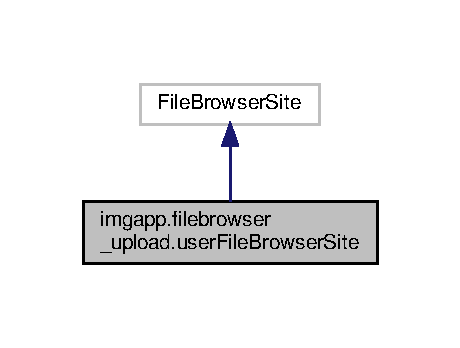
\includegraphics[width=221pt]{classimgapp_1_1filebrowser__upload_1_1userFileBrowserSite__inherit__graph}
\end{center}
\end{figure}


Collaboration diagram for imgapp.\+filebrowser\+\_\+upload.\+user\+File\+Browser\+Site\+:
\nopagebreak
\begin{figure}[H]
\begin{center}
\leavevmode
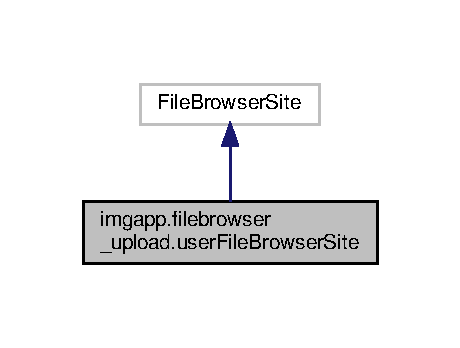
\includegraphics[width=221pt]{classimgapp_1_1filebrowser__upload_1_1userFileBrowserSite__coll__graph}
\end{center}
\end{figure}
\subsection*{Public Member Functions}
\begin{DoxyCompactItemize}
\item 
def \hyperlink{classimgapp_1_1filebrowser__upload_1_1userFileBrowserSite_ae8621cf07e7a542bde67af9ab97790f6}{upload} (self, request)
\begin{DoxyCompactList}\small\item\em override upload method from filebrowser, timestamp set whenever upload template is rendered \end{DoxyCompactList}\item 
def \hyperlink{classimgapp_1_1filebrowser__upload_1_1userFileBrowserSite_a847a2908ba1f3d28474de936665d823b}{delete} (self, request)
\begin{DoxyCompactList}\small\item\em override delete method, delete documents from mongo\+DB while deleting \end{DoxyCompactList}\end{DoxyCompactItemize}
\subsection*{Public Attributes}
\begin{DoxyCompactItemize}
\item 
\hyperlink{classimgapp_1_1filebrowser__upload_1_1userFileBrowserSite_a5cb7a63f6afb189b8060a533118630ef}{timestamp}
\end{DoxyCompactItemize}
\subsection*{Static Public Attributes}
\begin{DoxyCompactItemize}
\item 
string \hyperlink{classimgapp_1_1filebrowser__upload_1_1userFileBrowserSite_a540a50bf0a1b36907fc23a87a33f7f43}{timestamp} = \char`\"{}\char`\"{}
\begin{DoxyCompactList}\small\item\em upload timestamp, set when upload page is loaded \end{DoxyCompactList}\end{DoxyCompactItemize}
\subsection*{Private Member Functions}
\begin{DoxyCompactItemize}
\item 
def \hyperlink{classimgapp_1_1filebrowser__upload_1_1userFileBrowserSite_aeecdb2b8f77f56957df3bb8ab3ae6efd}{\+\_\+upload\+\_\+file} (self, request)
\begin{DoxyCompactList}\small\item\em override \+\_\+upload\+\_\+file method, updates the mongo\+DB with the meta-\/data of the images uploaded \end{DoxyCompactList}\end{DoxyCompactItemize}


\subsection{Detailed Description}
Override filebrowser site functionalities. 

\subsection{Member Function Documentation}
\mbox{\Hypertarget{classimgapp_1_1filebrowser__upload_1_1userFileBrowserSite_aeecdb2b8f77f56957df3bb8ab3ae6efd}\label{classimgapp_1_1filebrowser__upload_1_1userFileBrowserSite_aeecdb2b8f77f56957df3bb8ab3ae6efd}} 
\index{imgapp\+::filebrowser\+\_\+upload\+::user\+File\+Browser\+Site@{imgapp\+::filebrowser\+\_\+upload\+::user\+File\+Browser\+Site}!\+\_\+upload\+\_\+file@{\+\_\+upload\+\_\+file}}
\index{\+\_\+upload\+\_\+file@{\+\_\+upload\+\_\+file}!imgapp\+::filebrowser\+\_\+upload\+::user\+File\+Browser\+Site@{imgapp\+::filebrowser\+\_\+upload\+::user\+File\+Browser\+Site}}
\subsubsection{\texorpdfstring{\+\_\+upload\+\_\+file()}{\_upload\_file()}}
{\footnotesize\ttfamily def imgapp.\+filebrowser\+\_\+upload.\+user\+File\+Browser\+Site.\+\_\+upload\+\_\+file (\begin{DoxyParamCaption}\item[{}]{self,  }\item[{}]{request }\end{DoxyParamCaption})\hspace{0.3cm}{\ttfamily [private]}}



override \+\_\+upload\+\_\+file method, updates the mongo\+DB with the meta-\/data of the images uploaded 


\begin{DoxyParams}{Parameters}
{\em self} & reference to it\textquotesingle{}s own object \\
\hline
{\em request} & http request \\
\hline
\end{DoxyParams}
\mbox{\Hypertarget{classimgapp_1_1filebrowser__upload_1_1userFileBrowserSite_a847a2908ba1f3d28474de936665d823b}\label{classimgapp_1_1filebrowser__upload_1_1userFileBrowserSite_a847a2908ba1f3d28474de936665d823b}} 
\index{imgapp\+::filebrowser\+\_\+upload\+::user\+File\+Browser\+Site@{imgapp\+::filebrowser\+\_\+upload\+::user\+File\+Browser\+Site}!delete@{delete}}
\index{delete@{delete}!imgapp\+::filebrowser\+\_\+upload\+::user\+File\+Browser\+Site@{imgapp\+::filebrowser\+\_\+upload\+::user\+File\+Browser\+Site}}
\subsubsection{\texorpdfstring{delete()}{delete()}}
{\footnotesize\ttfamily def imgapp.\+filebrowser\+\_\+upload.\+user\+File\+Browser\+Site.\+delete (\begin{DoxyParamCaption}\item[{}]{self,  }\item[{}]{request }\end{DoxyParamCaption})}



override delete method, delete documents from mongo\+DB while deleting 


\begin{DoxyParams}{Parameters}
{\em self} & reference to it\textquotesingle{}s own object \\
\hline
{\em request} & http request \\
\hline
\end{DoxyParams}
\mbox{\Hypertarget{classimgapp_1_1filebrowser__upload_1_1userFileBrowserSite_ae8621cf07e7a542bde67af9ab97790f6}\label{classimgapp_1_1filebrowser__upload_1_1userFileBrowserSite_ae8621cf07e7a542bde67af9ab97790f6}} 
\index{imgapp\+::filebrowser\+\_\+upload\+::user\+File\+Browser\+Site@{imgapp\+::filebrowser\+\_\+upload\+::user\+File\+Browser\+Site}!upload@{upload}}
\index{upload@{upload}!imgapp\+::filebrowser\+\_\+upload\+::user\+File\+Browser\+Site@{imgapp\+::filebrowser\+\_\+upload\+::user\+File\+Browser\+Site}}
\subsubsection{\texorpdfstring{upload()}{upload()}}
{\footnotesize\ttfamily def imgapp.\+filebrowser\+\_\+upload.\+user\+File\+Browser\+Site.\+upload (\begin{DoxyParamCaption}\item[{}]{self,  }\item[{}]{request }\end{DoxyParamCaption})}



override upload method from filebrowser, timestamp set whenever upload template is rendered 


\begin{DoxyParams}{Parameters}
{\em self} & reference to it\textquotesingle{}s own object \\
\hline
{\em request} & http request \\
\hline
\end{DoxyParams}


\subsection{Member Data Documentation}
\mbox{\Hypertarget{classimgapp_1_1filebrowser__upload_1_1userFileBrowserSite_a540a50bf0a1b36907fc23a87a33f7f43}\label{classimgapp_1_1filebrowser__upload_1_1userFileBrowserSite_a540a50bf0a1b36907fc23a87a33f7f43}} 
\index{imgapp\+::filebrowser\+\_\+upload\+::user\+File\+Browser\+Site@{imgapp\+::filebrowser\+\_\+upload\+::user\+File\+Browser\+Site}!timestamp@{timestamp}}
\index{timestamp@{timestamp}!imgapp\+::filebrowser\+\_\+upload\+::user\+File\+Browser\+Site@{imgapp\+::filebrowser\+\_\+upload\+::user\+File\+Browser\+Site}}
\subsubsection{\texorpdfstring{timestamp}{timestamp}\hspace{0.1cm}{\footnotesize\ttfamily [1/2]}}
{\footnotesize\ttfamily string imgapp.\+filebrowser\+\_\+upload.\+user\+File\+Browser\+Site.\+timestamp = \char`\"{}\char`\"{}\hspace{0.3cm}{\ttfamily [static]}}



upload timestamp, set when upload page is loaded 

\mbox{\Hypertarget{classimgapp_1_1filebrowser__upload_1_1userFileBrowserSite_a5cb7a63f6afb189b8060a533118630ef}\label{classimgapp_1_1filebrowser__upload_1_1userFileBrowserSite_a5cb7a63f6afb189b8060a533118630ef}} 
\index{imgapp\+::filebrowser\+\_\+upload\+::user\+File\+Browser\+Site@{imgapp\+::filebrowser\+\_\+upload\+::user\+File\+Browser\+Site}!timestamp@{timestamp}}
\index{timestamp@{timestamp}!imgapp\+::filebrowser\+\_\+upload\+::user\+File\+Browser\+Site@{imgapp\+::filebrowser\+\_\+upload\+::user\+File\+Browser\+Site}}
\subsubsection{\texorpdfstring{timestamp}{timestamp}\hspace{0.1cm}{\footnotesize\ttfamily [2/2]}}
{\footnotesize\ttfamily imgapp.\+filebrowser\+\_\+upload.\+user\+File\+Browser\+Site.\+timestamp}



The documentation for this class was generated from the following file\+:\begin{DoxyCompactItemize}
\item 
imgapp/\hyperlink{filebrowser__upload_8py}{filebrowser\+\_\+upload.\+py}\end{DoxyCompactItemize}

\hypertarget{classimgapp_1_1forms_1_1UserForm}{}\section{imgapp.\+forms.\+User\+Form Class Reference}
\label{classimgapp_1_1forms_1_1UserForm}\index{imgapp.\+forms.\+User\+Form@{imgapp.\+forms.\+User\+Form}}


\hyperlink{classimgapp_1_1forms_1_1UserForm}{User\+Form}.  




Inheritance diagram for imgapp.\+forms.\+User\+Form\+:\nopagebreak
\begin{figure}[H]
\begin{center}
\leavevmode
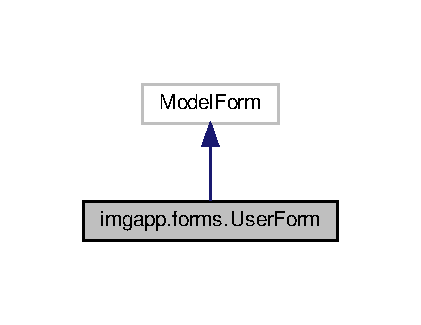
\includegraphics[width=202pt]{classimgapp_1_1forms_1_1UserForm__inherit__graph}
\end{center}
\end{figure}


Collaboration diagram for imgapp.\+forms.\+User\+Form\+:\nopagebreak
\begin{figure}[H]
\begin{center}
\leavevmode
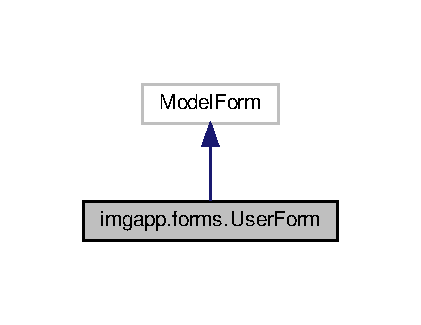
\includegraphics[width=202pt]{classimgapp_1_1forms_1_1UserForm__coll__graph}
\end{center}
\end{figure}
\subsection*{Classes}
\begin{DoxyCompactItemize}
\item 
class \hyperlink{classimgapp_1_1forms_1_1UserForm_1_1Meta}{Meta}
\begin{DoxyCompactList}\small\item\em meta class \end{DoxyCompactList}\end{DoxyCompactItemize}


\subsection{Detailed Description}
\hyperlink{classimgapp_1_1forms_1_1UserForm}{User\+Form}. 

Extends Model\+Form.~\newline
 Uses django User model.~\newline
 Form fields are username, password and email.~\newline
 Used in Sign Up form. 

The documentation for this class was generated from the following file\+:\begin{DoxyCompactItemize}
\item 
imgapp/\hyperlink{forms_8py}{forms.\+py}\end{DoxyCompactItemize}

\hypertarget{classimgapp_1_1utils_1_1Utils}{}\section{imgapp.\+utils.\+Utils Class Reference}
\label{classimgapp_1_1utils_1_1Utils}\index{imgapp.\+utils.\+Utils@{imgapp.\+utils.\+Utils}}


darknet model class  


\subsection*{Public Member Functions}
\begin{DoxyCompactItemize}
\item 
def \hyperlink{classimgapp_1_1utils_1_1Utils_aace6e93f019f79968dd5c0b14b09eb70}{\+\_\+\+\_\+init\+\_\+\+\_\+} (self)
\begin{DoxyCompactList}\small\item\em constructor \end{DoxyCompactList}\item 
def \hyperlink{classimgapp_1_1utils_1_1Utils_aceeb858cb98ce6b5f7aa1d5e2c599490}{get\+\_\+bounding\+Box} (self, img)
\begin{DoxyCompactList}\small\item\em Wrap around image in darknet format and forward pass. \end{DoxyCompactList}\end{DoxyCompactItemize}
\subsection*{Public Attributes}
\begin{DoxyCompactItemize}
\item 
\hyperlink{classimgapp_1_1utils_1_1Utils_a421da25276568d870b9f3347dfdea33e}{net}
\item 
\hyperlink{classimgapp_1_1utils_1_1Utils_adb7539784726cf1477e24ed2433e6f72}{detection\+\_\+threshold}
\end{DoxyCompactItemize}


\subsection{Detailed Description}
darknet model class 

includes all darknet model functionalities 

\subsection{Constructor \& Destructor Documentation}
\mbox{\Hypertarget{classimgapp_1_1utils_1_1Utils_aace6e93f019f79968dd5c0b14b09eb70}\label{classimgapp_1_1utils_1_1Utils_aace6e93f019f79968dd5c0b14b09eb70}} 
\index{imgapp\+::utils\+::\+Utils@{imgapp\+::utils\+::\+Utils}!\+\_\+\+\_\+init\+\_\+\+\_\+@{\+\_\+\+\_\+init\+\_\+\+\_\+}}
\index{\+\_\+\+\_\+init\+\_\+\+\_\+@{\+\_\+\+\_\+init\+\_\+\+\_\+}!imgapp\+::utils\+::\+Utils@{imgapp\+::utils\+::\+Utils}}
\subsubsection{\texorpdfstring{\+\_\+\+\_\+init\+\_\+\+\_\+()}{\_\_init\_\_()}}
{\footnotesize\ttfamily def imgapp.\+utils.\+Utils.\+\_\+\+\_\+init\+\_\+\+\_\+ (\begin{DoxyParamCaption}\item[{}]{self }\end{DoxyParamCaption})}



constructor 


\begin{DoxyParams}{Parameters}
{\em self} & reference to it\textquotesingle{}s own object \\
\hline
\end{DoxyParams}


\subsection{Member Function Documentation}
\mbox{\Hypertarget{classimgapp_1_1utils_1_1Utils_aceeb858cb98ce6b5f7aa1d5e2c599490}\label{classimgapp_1_1utils_1_1Utils_aceeb858cb98ce6b5f7aa1d5e2c599490}} 
\index{imgapp\+::utils\+::\+Utils@{imgapp\+::utils\+::\+Utils}!get\+\_\+bounding\+Box@{get\+\_\+bounding\+Box}}
\index{get\+\_\+bounding\+Box@{get\+\_\+bounding\+Box}!imgapp\+::utils\+::\+Utils@{imgapp\+::utils\+::\+Utils}}
\subsubsection{\texorpdfstring{get\+\_\+bounding\+Box()}{get\_boundingBox()}}
{\footnotesize\ttfamily def imgapp.\+utils.\+Utils.\+get\+\_\+bounding\+Box (\begin{DoxyParamCaption}\item[{}]{self,  }\item[{}]{img }\end{DoxyParamCaption})}



Wrap around image in darknet format and forward pass. 


\begin{DoxyParams}{Parameters}
{\em self} & reference to it\textquotesingle{}s own object \\
\hline
{\em img} & image matrix \\
\hline
\end{DoxyParams}


\subsection{Member Data Documentation}
\mbox{\Hypertarget{classimgapp_1_1utils_1_1Utils_adb7539784726cf1477e24ed2433e6f72}\label{classimgapp_1_1utils_1_1Utils_adb7539784726cf1477e24ed2433e6f72}} 
\index{imgapp\+::utils\+::\+Utils@{imgapp\+::utils\+::\+Utils}!detection\+\_\+threshold@{detection\+\_\+threshold}}
\index{detection\+\_\+threshold@{detection\+\_\+threshold}!imgapp\+::utils\+::\+Utils@{imgapp\+::utils\+::\+Utils}}
\subsubsection{\texorpdfstring{detection\+\_\+threshold}{detection\_threshold}}
{\footnotesize\ttfamily imgapp.\+utils.\+Utils.\+detection\+\_\+threshold}

\mbox{\Hypertarget{classimgapp_1_1utils_1_1Utils_a421da25276568d870b9f3347dfdea33e}\label{classimgapp_1_1utils_1_1Utils_a421da25276568d870b9f3347dfdea33e}} 
\index{imgapp\+::utils\+::\+Utils@{imgapp\+::utils\+::\+Utils}!net@{net}}
\index{net@{net}!imgapp\+::utils\+::\+Utils@{imgapp\+::utils\+::\+Utils}}
\subsubsection{\texorpdfstring{net}{net}}
{\footnotesize\ttfamily imgapp.\+utils.\+Utils.\+net}



The documentation for this class was generated from the following file\+:\begin{DoxyCompactItemize}
\item 
imgapp/\hyperlink{utils_8py}{utils.\+py}\end{DoxyCompactItemize}

\chapter{File Documentation}
\hypertarget{____init_____8py}{}\section{imgapp/\+\_\+\+\_\+init\+\_\+\+\_\+.py File Reference}
\label{____init_____8py}\index{imgapp/\+\_\+\+\_\+init\+\_\+\+\_\+.\+py@{imgapp/\+\_\+\+\_\+init\+\_\+\+\_\+.\+py}}
\subsection*{Namespaces}
\begin{DoxyCompactItemize}
\item 
 \hyperlink{namespaceimgapp}{imgapp}
\end{DoxyCompactItemize}

\hypertarget{migrations_2____init_____8py}{}\section{imgapp/migrations/\+\_\+\+\_\+init\+\_\+\+\_\+.py File Reference}
\label{migrations_2____init_____8py}\index{imgapp/migrations/\+\_\+\+\_\+init\+\_\+\+\_\+.\+py@{imgapp/migrations/\+\_\+\+\_\+init\+\_\+\+\_\+.\+py}}
\subsection*{Namespaces}
\begin{DoxyCompactItemize}
\item 
 \hyperlink{namespaceimgapp_1_1migrations}{imgapp.\+migrations}
\end{DoxyCompactItemize}

\hypertarget{admin_8py}{}\section{imgapp/admin.py File Reference}
\label{admin_8py}\index{imgapp/admin.\+py@{imgapp/admin.\+py}}
\subsection*{Namespaces}
\begin{DoxyCompactItemize}
\item 
 \hyperlink{namespaceimgapp_1_1admin}{imgapp.\+admin}
\item 
 \hyperlink{namespaceadmin}{admin}
\begin{DoxyCompactList}\small\item\em register models at admin \end{DoxyCompactList}\end{DoxyCompactItemize}

\hypertarget{apps_8py}{}\section{imgapp/apps.py File Reference}
\label{apps_8py}\index{imgapp/apps.\+py@{imgapp/apps.\+py}}
\subsection*{Classes}
\begin{DoxyCompactItemize}
\item 
class \hyperlink{classimgapp_1_1apps_1_1ImgappConfig}{imgapp.\+apps.\+Imgapp\+Config}
\begin{DoxyCompactList}\small\item\em imgapp A\+PI class \end{DoxyCompactList}\end{DoxyCompactItemize}
\subsection*{Namespaces}
\begin{DoxyCompactItemize}
\item 
 \hyperlink{namespaceimgapp_1_1apps}{imgapp.\+apps}
\item 
 \hyperlink{namespaceapps}{apps}
\begin{DoxyCompactList}\small\item\em imgapp app class \end{DoxyCompactList}\end{DoxyCompactItemize}

\hypertarget{ExtractExif_8py}{}\section{imgapp/\+Extract\+Exif.py File Reference}
\label{ExtractExif_8py}\index{imgapp/\+Extract\+Exif.\+py@{imgapp/\+Extract\+Exif.\+py}}
\subsection*{Classes}
\begin{DoxyCompactItemize}
\item 
class \hyperlink{classimgapp_1_1ExtractExif_1_1Extract__Exif}{imgapp.\+Extract\+Exif.\+Extract\+\_\+\+Exif}
\begin{DoxyCompactList}\small\item\em \hyperlink{classimgapp_1_1ExtractExif_1_1Extract__Exif}{Extract\+\_\+\+Exif} class. \end{DoxyCompactList}\end{DoxyCompactItemize}
\subsection*{Namespaces}
\begin{DoxyCompactItemize}
\item 
 \hyperlink{namespaceimgapp_1_1ExtractExif}{imgapp.\+Extract\+Exif}
\item 
 \hyperlink{namespaceExtractExif}{Extract\+Exif}
\begin{DoxyCompactList}\small\item\em extract meta-\/data from images. \end{DoxyCompactList}\end{DoxyCompactItemize}

\hypertarget{filebrowser__upload_8py}{}\section{imgapp/filebrowser\+\_\+upload.py File Reference}
\label{filebrowser__upload_8py}\index{imgapp/filebrowser\+\_\+upload.\+py@{imgapp/filebrowser\+\_\+upload.\+py}}
\subsection*{Classes}
\begin{DoxyCompactItemize}
\item 
class \hyperlink{classimgapp_1_1filebrowser__upload_1_1userFileBrowserSite}{imgapp.\+filebrowser\+\_\+upload.\+user\+File\+Browser\+Site}
\begin{DoxyCompactList}\small\item\em Override filebrowser site functionalities. \end{DoxyCompactList}\end{DoxyCompactItemize}
\subsection*{Namespaces}
\begin{DoxyCompactItemize}
\item 
 \hyperlink{namespaceimgapp_1_1filebrowser__upload}{imgapp.\+filebrowser\+\_\+upload}
\item 
 \hyperlink{namespacefilebrowser__upload}{filebrowser\+\_\+upload}
\begin{DoxyCompactList}\small\item\em override the filebrowser site functionalities \end{DoxyCompactList}\end{DoxyCompactItemize}
\subsection*{Variables}
\begin{DoxyCompactItemize}
\item 
\hyperlink{namespaceimgapp_1_1filebrowser__upload_ae26049c70fbfba51dec84d62840e6a01}{imgapp.\+filebrowser\+\_\+upload.\+storage} = Default\+Storage()
\item 
\hyperlink{namespaceimgapp_1_1filebrowser__upload_a4f8619d5576e067e06247f18cd273af8}{imgapp.\+filebrowser\+\_\+upload.\+site} = user\+File\+Browser\+Site(name=\textquotesingle{}filebrowser\textquotesingle{}, storage=storage)
\end{DoxyCompactItemize}

\hypertarget{forms_8py}{}\section{imgapp/forms.py File Reference}
\label{forms_8py}\index{imgapp/forms.\+py@{imgapp/forms.\+py}}
\subsection*{Classes}
\begin{DoxyCompactItemize}
\item 
class \hyperlink{classimgapp_1_1forms_1_1UserForm}{imgapp.\+forms.\+User\+Form}
\begin{DoxyCompactList}\small\item\em \hyperlink{classimgapp_1_1forms_1_1UserForm}{User\+Form}. \end{DoxyCompactList}\item 
class \hyperlink{classimgapp_1_1forms_1_1UserForm_1_1Meta}{imgapp.\+forms.\+User\+Form.\+Meta}
\begin{DoxyCompactList}\small\item\em meta class \end{DoxyCompactList}\item 
class \hyperlink{classimgapp_1_1forms_1_1ProfileForm}{imgapp.\+forms.\+Profile\+Form}
\begin{DoxyCompactList}\small\item\em \hyperlink{classimgapp_1_1forms_1_1ProfileForm}{Profile\+Form}. \end{DoxyCompactList}\item 
class \hyperlink{classimgapp_1_1forms_1_1ProfileForm_1_1Meta}{imgapp.\+forms.\+Profile\+Form.\+Meta}
\begin{DoxyCompactList}\small\item\em meta class \end{DoxyCompactList}\end{DoxyCompactItemize}
\subsection*{Namespaces}
\begin{DoxyCompactItemize}
\item 
 \hyperlink{namespaceimgapp_1_1forms}{imgapp.\+forms}
\item 
 \hyperlink{namespaceforms}{forms}
\begin{DoxyCompactList}\small\item\em model forms \end{DoxyCompactList}\end{DoxyCompactItemize}

\hypertarget{0001__initial_8py}{}\section{imgapp/migrations/0001\+\_\+initial.py File Reference}
\label{0001__initial_8py}\index{imgapp/migrations/0001\+\_\+initial.\+py@{imgapp/migrations/0001\+\_\+initial.\+py}}
\subsection*{Classes}
\begin{DoxyCompactItemize}
\item 
class \hyperlink{classimgapp_1_1migrations_1_10001__initial_1_1Migration}{imgapp.\+migrations.\+0001\+\_\+initial.\+Migration}
\end{DoxyCompactItemize}
\subsection*{Namespaces}
\begin{DoxyCompactItemize}
\item 
 \hyperlink{namespaceimgapp_1_1migrations_1_10001__initial}{imgapp.\+migrations.\+0001\+\_\+initial}
\end{DoxyCompactItemize}

\hypertarget{0002__objects_8py}{}\section{imgapp/migrations/0002\+\_\+objects.py File Reference}
\label{0002__objects_8py}\index{imgapp/migrations/0002\+\_\+objects.\+py@{imgapp/migrations/0002\+\_\+objects.\+py}}
\subsection*{Classes}
\begin{DoxyCompactItemize}
\item 
class \hyperlink{classimgapp_1_1migrations_1_10002__objects_1_1Migration}{imgapp.\+migrations.\+0002\+\_\+objects.\+Migration}
\end{DoxyCompactItemize}
\subsection*{Namespaces}
\begin{DoxyCompactItemize}
\item 
 \hyperlink{namespaceimgapp_1_1migrations_1_10002__objects}{imgapp.\+migrations.\+0002\+\_\+objects}
\end{DoxyCompactItemize}

\hypertarget{0003__description_8py}{}\section{imgapp/migrations/0003\+\_\+description.py File Reference}
\label{0003__description_8py}\index{imgapp/migrations/0003\+\_\+description.\+py@{imgapp/migrations/0003\+\_\+description.\+py}}
\subsection*{Classes}
\begin{DoxyCompactItemize}
\item 
class \hyperlink{classimgapp_1_1migrations_1_10003__description_1_1Migration}{imgapp.\+migrations.\+0003\+\_\+description.\+Migration}
\end{DoxyCompactItemize}
\subsection*{Namespaces}
\begin{DoxyCompactItemize}
\item 
 \hyperlink{namespaceimgapp_1_1migrations_1_10003__description}{imgapp.\+migrations.\+0003\+\_\+description}
\end{DoxyCompactItemize}

\hypertarget{0004__auto__20190715__1327_8py}{}\section{imgapp/migrations/0004\+\_\+auto\+\_\+20190715\+\_\+1327.py File Reference}
\label{0004__auto__20190715__1327_8py}\index{imgapp/migrations/0004\+\_\+auto\+\_\+20190715\+\_\+1327.\+py@{imgapp/migrations/0004\+\_\+auto\+\_\+20190715\+\_\+1327.\+py}}
\subsection*{Classes}
\begin{DoxyCompactItemize}
\item 
class \hyperlink{classimgapp_1_1migrations_1_10004__auto__20190715__1327_1_1Migration}{imgapp.\+migrations.\+0004\+\_\+auto\+\_\+20190715\+\_\+1327.\+Migration}
\end{DoxyCompactItemize}
\subsection*{Namespaces}
\begin{DoxyCompactItemize}
\item 
 \hyperlink{namespaceimgapp_1_1migrations_1_10004__auto__20190715__1327}{imgapp.\+migrations.\+0004\+\_\+auto\+\_\+20190715\+\_\+1327}
\end{DoxyCompactItemize}

\hypertarget{models_8py}{}\section{imgapp/models.py File Reference}
\label{models_8py}\index{imgapp/models.\+py@{imgapp/models.\+py}}
\subsection*{Classes}
\begin{DoxyCompactItemize}
\item 
class \hyperlink{classimgapp_1_1models_1_1Profile}{imgapp.\+models.\+Profile}
\begin{DoxyCompactList}\small\item\em User \hyperlink{classimgapp_1_1models_1_1Profile}{Profile}. \end{DoxyCompactList}\end{DoxyCompactItemize}
\subsection*{Namespaces}
\begin{DoxyCompactItemize}
\item 
 \hyperlink{namespaceimgapp_1_1models}{imgapp.\+models}
\item 
 \hyperlink{namespacemodels}{models}
\begin{DoxyCompactList}\small\item\em Create your models here. \end{DoxyCompactList}\end{DoxyCompactItemize}

\hypertarget{MongoQuery_8py}{}\section{imgapp/\+Mongo\+Query.py File Reference}
\label{MongoQuery_8py}\index{imgapp/\+Mongo\+Query.\+py@{imgapp/\+Mongo\+Query.\+py}}
\subsection*{Classes}
\begin{DoxyCompactItemize}
\item 
class \hyperlink{classimgapp_1_1MongoQuery_1_1mongoQuery}{imgapp.\+Mongo\+Query.\+mongo\+Query}
\begin{DoxyCompactList}\small\item\em Class to query mongo\+DB. \end{DoxyCompactList}\end{DoxyCompactItemize}
\subsection*{Namespaces}
\begin{DoxyCompactItemize}
\item 
 \hyperlink{namespaceimgapp_1_1MongoQuery}{imgapp.\+Mongo\+Query}
\item 
 \hyperlink{namespacemongoQuery}{mongo\+Query}
\begin{DoxyCompactList}\small\item\em module to query on mongo\+DB \end{DoxyCompactList}\end{DoxyCompactItemize}
\subsection*{Functions}
\begin{DoxyCompactItemize}
\item 
def \hyperlink{namespaceimgapp_1_1MongoQuery_aa2f709bf0b0e267cfb513e326bbc6e4d}{imgapp.\+Mongo\+Query.\+append\+ID} (image, imageids)
\begin{DoxyCompactList}\small\item\em specially used for coco; find coco image id and append it to imageids \end{DoxyCompactList}\end{DoxyCompactItemize}
\subsection*{Variables}
\begin{DoxyCompactItemize}
\item 
\hyperlink{namespaceimgapp_1_1MongoQuery_a3c845d9e355454c43db2eca20b9058bb}{imgapp.\+Mongo\+Query.\+Query} = mongo\+Query()
\end{DoxyCompactItemize}

\hypertarget{tests_8py}{}\section{imgapp/tests.py File Reference}
\label{tests_8py}\index{imgapp/tests.\+py@{imgapp/tests.\+py}}
\subsection*{Namespaces}
\begin{DoxyCompactItemize}
\item 
 \hyperlink{namespaceimgapp_1_1tests}{imgapp.\+tests}
\end{DoxyCompactItemize}

\hypertarget{UpdateMongoDB_8py}{}\section{imgapp/\+Update\+Mongo\+DB.py File Reference}
\label{UpdateMongoDB_8py}\index{imgapp/\+Update\+Mongo\+D\+B.\+py@{imgapp/\+Update\+Mongo\+D\+B.\+py}}
\subsection*{Namespaces}
\begin{DoxyCompactItemize}
\item 
 \hyperlink{namespaceimgapp_1_1UpdateMongoDB}{imgapp.\+Update\+Mongo\+DB}
\item 
 \hyperlink{namespaceUpdateMongoDB}{Update\+Mongo\+DB}
\begin{DoxyCompactList}\small\item\em utilities to update documents in Mongo\+DB \end{DoxyCompactList}\end{DoxyCompactItemize}
\subsection*{Functions}
\begin{DoxyCompactItemize}
\item 
def \hyperlink{namespaceimgapp_1_1UpdateMongoDB_a5bc486192c38922a65cc60e598bc9b1e}{imgapp.\+Update\+Mongo\+D\+B.\+update\+\_\+\+Mongo} (Image\+Type, Path, timestamp, user\+ID, is\+\_\+file\+\_\+flag)
\begin{DoxyCompactList}\small\item\em upload file\textquotesingle{}s meta-\/data to mongo\+DB \end{DoxyCompactList}\item 
def \hyperlink{namespaceimgapp_1_1UpdateMongoDB_aa239083b46ac5a0d725fa61e8068553b}{imgapp.\+Update\+Mongo\+D\+B.\+delete\+\_\+\+User\+\_\+\+Collection} (user\+ID)
\begin{DoxyCompactList}\small\item\em drop user collection, not functioning with this imanage branch, but given here for reference issue\+: user filebrowser folders are not different \end{DoxyCompactList}\item 
def \hyperlink{namespaceimgapp_1_1UpdateMongoDB_ac48df6f990520cda63813e27faa06095}{imgapp.\+Update\+Mongo\+D\+B.\+delete\+\_\+file\+\_\+data} (is\+\_\+file\+\_\+flag, path, user\+ID)
\begin{DoxyCompactList}\small\item\em delete documents from mongo\+DB, used in the delete method of User\+File\+Browser\+Site class \end{DoxyCompactList}\end{DoxyCompactItemize}
\subsection*{Variables}
\begin{DoxyCompactItemize}
\item 
\hyperlink{namespaceimgapp_1_1UpdateMongoDB_a5b8548ed7b19bb6f553a7c052c778406}{imgapp.\+Update\+Mongo\+D\+B.\+Utils\+\_\+\+Object} = Utils()
\begin{DoxyCompactList}\small\item\em Uitls object \+: instance of the model. \end{DoxyCompactList}\item 
def \hyperlink{namespaceimgapp_1_1UpdateMongoDB_ae23d58bb055998ec921a4a52cdc001f9}{imgapp.\+Update\+Mongo\+D\+B.\+items} = update\+\_\+\+Mongo(\textquotesingle{}\textquotesingle{})
\end{DoxyCompactItemize}

\hypertarget{uploadCOCO_8py}{}\section{imgapp/upload\+C\+O\+CO.py File Reference}
\label{uploadCOCO_8py}\index{imgapp/upload\+C\+O\+C\+O.\+py@{imgapp/upload\+C\+O\+C\+O.\+py}}
\subsection*{Namespaces}
\begin{DoxyCompactItemize}
\item 
 \hyperlink{namespaceimgapp_1_1uploadCOCO}{imgapp.\+upload\+C\+O\+CO}
\end{DoxyCompactItemize}
\subsection*{Functions}
\begin{DoxyCompactItemize}
\item 
def \hyperlink{namespaceimgapp_1_1uploadCOCO_a00079a30241831574eb416c09fef0bbc}{imgapp.\+upload\+C\+O\+C\+O.\+make\+\_\+imgname} (imgid)
\begin{DoxyCompactList}\small\item\em return imagename out of the image id \end{DoxyCompactList}\item 
def \hyperlink{namespaceimgapp_1_1uploadCOCO_ac33f4c865b41867bda1f5197dab6f808}{imgapp.\+upload\+C\+O\+C\+O.\+get\+Cat\+\_\+info} (category, cat\+\_\+id)
\begin{DoxyCompactList}\small\item\em returns category info in a dictionary using the category ID \end{DoxyCompactList}\item 
def \hyperlink{namespaceimgapp_1_1uploadCOCO_ad068eaf76576fa93dc00dcd4082bed86}{imgapp.\+upload\+C\+O\+C\+O.\+List\+Objects} (annotations\+\_\+list, category)
\begin{DoxyCompactList}\small\item\em map all objects in a image and returns dictionary with image name as the key and objects list as the value \end{DoxyCompactList}\item 
def \hyperlink{namespaceimgapp_1_1uploadCOCO_a43518ccef3fb3c5b5afac1881a520292}{imgapp.\+upload\+C\+O\+C\+O.\+upload\+C\+O\+CO} ()
\begin{DoxyCompactList}\small\item\em call this fucntion to upload images, Note \+: change the path to the directory with C\+O\+CO images \end{DoxyCompactList}\end{DoxyCompactItemize}

\hypertarget{uploadThreadClass_8py}{}\section{imgapp/upload\+Thread\+Class.py File Reference}
\label{uploadThreadClass_8py}\index{imgapp/upload\+Thread\+Class.\+py@{imgapp/upload\+Thread\+Class.\+py}}
\subsection*{Classes}
\begin{DoxyCompactItemize}
\item 
class \hyperlink{classimgapp_1_1uploadThreadClass_1_1UpdateMongo__Thread}{imgapp.\+upload\+Thread\+Class.\+Update\+Mongo\+\_\+\+Thread}
\begin{DoxyCompactList}\small\item\em Class to update mongo\+DB. \end{DoxyCompactList}\end{DoxyCompactItemize}
\subsection*{Namespaces}
\begin{DoxyCompactItemize}
\item 
 \hyperlink{namespaceimgapp_1_1uploadThreadClass}{imgapp.\+upload\+Thread\+Class}
\item 
 \hyperlink{namespaceuploadThreadClass}{upload\+Thread\+Class}
\begin{DoxyCompactList}\small\item\em upload the metra data in a separate thread, (not being used in this imanage branch) \end{DoxyCompactList}\end{DoxyCompactItemize}

\hypertarget{urls_8py}{}\section{imgapp/urls.py File Reference}
\label{urls_8py}\index{imgapp/urls.\+py@{imgapp/urls.\+py}}
\subsection*{Namespaces}
\begin{DoxyCompactItemize}
\item 
 \hyperlink{namespaceimgapp_1_1urls}{imgapp.\+urls}
\end{DoxyCompactItemize}

\hypertarget{utils_8py}{}\section{imgapp/utils.py File Reference}
\label{utils_8py}\index{imgapp/utils.\+py@{imgapp/utils.\+py}}
\subsection*{Classes}
\begin{DoxyCompactItemize}
\item 
class \hyperlink{classimgapp_1_1utils_1_1Utils}{imgapp.\+utils.\+Utils}
\begin{DoxyCompactList}\small\item\em darknet model class \end{DoxyCompactList}\end{DoxyCompactItemize}
\subsection*{Namespaces}
\begin{DoxyCompactItemize}
\item 
 \hyperlink{namespaceimgapp_1_1utils}{imgapp.\+utils}
\item 
 \hyperlink{namespaceutils}{utils}
\begin{DoxyCompactList}\small\item\em all C\+O\+CO and darknet model functionalities \end{DoxyCompactList}\end{DoxyCompactItemize}
\subsection*{Functions}
\begin{DoxyCompactItemize}
\item 
def \hyperlink{namespaceimgapp_1_1utils_a6d744ddd54588b6d14e6dc10b504e5c3}{imgapp.\+utils.\+set\+\_\+color} (names\+\_\+file)
\begin{DoxyCompactList}\small\item\em create color mapping with respect ot classes \end{DoxyCompactList}\item 
def \hyperlink{namespaceimgapp_1_1utils_a468cc459f9ea6c9c150db800f5d76212}{imgapp.\+utils.\+get\+\_\+color} (label)
\begin{DoxyCompactList}\small\item\em returns R\+GB values depending on class label \end{DoxyCompactList}\item 
def \hyperlink{namespaceimgapp_1_1utils_a7e2ce0fe32d261f7a8c57030029aa401}{imgapp.\+utils.\+draw\+\_\+bbox} (img, bounds, label)
\begin{DoxyCompactList}\small\item\em draw bounding boxes \end{DoxyCompactList}\item 
def \hyperlink{namespaceimgapp_1_1utils_ab0143c8cde7f9ee033d14b55642640f4}{imgapp.\+utils.\+save\+\_\+annotated\+File} (img\+Ids, cat\+\_\+names)
\begin{DoxyCompactList}\small\item\em make object annotations and save the resulting image, uses C\+O\+CO model \end{DoxyCompactList}\end{DoxyCompactItemize}
\subsection*{Variables}
\begin{DoxyCompactItemize}
\item 
dictionary \hyperlink{namespaceimgapp_1_1utils_aef6c0a613ef435057531c3e15d7ee228}{imgapp.\+utils.\+color\+\_\+map} = \{\}
\begin{DoxyCompactList}\small\item\em color mapping for bounding boxes \end{DoxyCompactList}\item 
\hyperlink{namespaceimgapp_1_1utils_ab8f7f09b0a834029cdce936a10744e75}{imgapp.\+utils.\+settings} = json.\+load(f)
\item 
\hyperlink{namespaceimgapp_1_1utils_a8e182872d7fd166b733945c31c6e75b0}{imgapp.\+utils.\+annfile} = settings\mbox{[}\char`\"{}coco\char`\"{}\mbox{]}\mbox{[}\char`\"{}ann\+\_\+file\char`\"{}\mbox{]}
\begin{DoxyCompactList}\small\item\em annotations file path used by coco \end{DoxyCompactList}\item 
\hyperlink{namespaceimgapp_1_1utils_a019aef0229f11d0fce25f09543158b1d}{imgapp.\+utils.\+coco} = C\+O\+CO(annfile)
\begin{DoxyCompactList}\small\item\em C\+O\+CO model instance. \end{DoxyCompactList}\item 
\hyperlink{namespaceimgapp_1_1utils_a76721855ae19d74f938f4a234ccf2fa4}{imgapp.\+utils.\+Cat} = coco.\+load\+Cats(coco.\+get\+Cat\+Ids())
\begin{DoxyCompactList}\small\item\em Category info. \end{DoxyCompactList}\end{DoxyCompactItemize}

\hypertarget{views_8py}{}\section{imgapp/views.py File Reference}
\label{views_8py}\index{imgapp/views.\+py@{imgapp/views.\+py}}
\subsection*{Namespaces}
\begin{DoxyCompactItemize}
\item 
 \hyperlink{namespaceimgapp_1_1views}{imgapp.\+views}
\item 
 \hyperlink{namespaceviews}{views}
\begin{DoxyCompactList}\small\item\em handle requested views \end{DoxyCompactList}\end{DoxyCompactItemize}
\subsection*{Functions}
\begin{DoxyCompactItemize}
\item 
def \hyperlink{namespaceimgapp_1_1views_adcf4ad535b76cf41f5894ad57bcdbc43}{imgapp.\+views.\+Form} (request)
\begin{DoxyCompactList}\small\item\em render upload images form template, not being used in imanage branch \end{DoxyCompactList}\item 
def \hyperlink{namespaceimgapp_1_1views_a30bd5c7a24785551afd3da58fa259a6b}{imgapp.\+views.\+Upload} (request)
\begin{DoxyCompactList}\small\item\em upload images after upload form is submitted, not being used in imanage branch \end{DoxyCompactList}\item 
def \hyperlink{namespaceimgapp_1_1views_a3e7e98b43ec1f6f0205f62d1ddcc505b}{imgapp.\+views.\+Updated\+Mongo} (request)
\begin{DoxyCompactList}\small\item\em images uploaded confirmation, not being used in imanage branch \end{DoxyCompactList}\item 
def \hyperlink{namespaceimgapp_1_1views_ad231247785394cfcbefcf27970310f64}{imgapp.\+views.\+delete} (request)
\begin{DoxyCompactList}\small\item\em drop user collection, not being used in the imanage branch \end{DoxyCompactList}\item 
def \hyperlink{namespaceimgapp_1_1views_a42d42280064441dcaa48088fe3e43222}{imgapp.\+views.\+Query\+Object} (request)
\begin{DoxyCompactList}\small\item\em query images form \end{DoxyCompactList}\item 
def \hyperlink{namespaceimgapp_1_1views_a0bad743f7a5c8bce58dbe6250dbc105f}{imgapp.\+views.\+format\+\_\+datetime} (time)
\begin{DoxyCompactList}\small\item\em format datetime (change \char`\"{}\%\+Y-\/\%\+M-\/\%\+D\+T\%\+H\+:\%\+M\char`\"{} to \char`\"{}\%\+Y-\/\%\+M-\/\%\+D \%\+H\+:\%\+M\+:\%\+S\char`\"{}) \end{DoxyCompactList}\item 
def \hyperlink{namespaceimgapp_1_1views_a06d5c0cac6ae36a355b522abb883932b}{imgapp.\+views.\+Query\+Object\+Result} (request)
\begin{DoxyCompactList}\small\item\em process query, search on Mongo\+DB and write the resulting template \end{DoxyCompactList}\item 
def \hyperlink{namespaceimgapp_1_1views_a6ce45040afbe69d047853cb4258a4761}{imgapp.\+views.\+Showresults\+\_\+\+Objects} (result)
\begin{DoxyCompactList}\small\item\em show results for the queries,modifies the template to show the required images \end{DoxyCompactList}\item 
def \hyperlink{namespaceimgapp_1_1views_a7ff46cd0d8d9cddbd78a488b2e45ce0c}{imgapp.\+views.\+Sign\+Up\+\_\+\+Form} (request)
\begin{DoxyCompactList}\small\item\em render sign\+\_\+up form and create staff user when form is submitted \end{DoxyCompactList}\item 
def \hyperlink{namespaceimgapp_1_1views_aad5f229f777ab6368cc67dab4436b8ac}{imgapp.\+views.\+description} (request)
\begin{DoxyCompactList}\small\item\em render description template \end{DoxyCompactList}\item 
def \hyperlink{namespaceimgapp_1_1views_a79dd171b98f07f4649cd2e44644ab8e0}{imgapp.\+views.\+view\+Image} (request)
\begin{DoxyCompactList}\small\item\em filebrowser view image \end{DoxyCompactList}\end{DoxyCompactItemize}
\subsection*{Variables}
\begin{DoxyCompactItemize}
\item 
string \hyperlink{namespaceimgapp_1_1views_ae3b2640fa382262bdf30df5509438d83}{imgapp.\+views.\+S\+T\+A\+T\+I\+C\+P\+A\+TH} = B\+A\+S\+E\+\_\+\+D\+IR+\textquotesingle{}/imgapp/static\textquotesingle{}
\begin{DoxyCompactList}\small\item\em static path \end{DoxyCompactList}\item 
\hyperlink{namespaceimgapp_1_1views_ace59bf1ee23e1e68ab25883a1ab83a07}{imgapp.\+views.\+objectslist} = json.\+load(f)
\begin{DoxyCompactList}\small\item\em objectslist = class names \end{DoxyCompactList}\end{DoxyCompactItemize}

%--- End generated contents ---

% Index
\backmatter
\newpage
\phantomsection
\clearemptydoublepage
\addcontentsline{toc}{chapter}{Index}
\printindex

\end{document}
